%&preformat-disser
\RequirePackage[l2tabu,orthodox]{nag} % Раскомментировав, можно в логе получать рекомендации относительно правильного использования пакетов и предупреждения об устаревших и нерекомендуемых пакетах
% Формат А4, 14pt (ГОСТ Р 7.0.11-2011, 5.3.6)
\documentclass[a4paper,14pt,oneside,openany]{memoir}

%%%%%%%%%%%%%%%%%%%%%%%%%%%%%%%%%%%%%%%%%%%%%%%%%%%%%%%%%%%%%%%%%%%%%%%%%%%%%%%%
%%%% Файл упрощённых настроек шаблона, общих для диссертации и автореферата %%%%
%%%%%%%%%%%%%%%%%%%%%%%%%%%%%%%%%%%%%%%%%%%%%%%%%%%%%%%%%%%%%%%%%%%%%%%%%%%%%%%%

%%% Режим черновика %%%
\makeatletter
\@ifundefined{c@draft}{
  \newcounter{draft}
  \setcounter{draft}{0}  % 0 --- чистовик (максимальное соблюдение ГОСТ)
                         % 1 --- черновик (отклонения от ГОСТ, но быстрая
                         %       сборка итоговых PDF)
}{}
\makeatother

%%% Пометки в тексте %%%
\makeatletter
\@ifundefined{c@showmarkup}{
  \newcounter{showmarkup}
  \setcounter{showmarkup}{0}  % 0 --- скрыть пометки
                              % 1 --- показывать пометки
}{}
\makeatother

%%% Использование в pdflatex шрифтов не по-умолчанию %%%
\makeatletter
\@ifundefined{c@usealtfont}{
  \newcounter{usealtfont}
  \setcounter{usealtfont}{1}    % 0 --- шрифты на базе Computer Modern
                                % 1 --- использовать пакет pscyr, при его
                                %       наличии
                                % 2 --- использовать пакет XCharter, при наличии
                                %       подходящей версии
}{}
\makeatother

%%% Использование в xelatex и lualatex семейств шрифтов %%%
\makeatletter
\@ifundefined{c@fontfamily}{
  \newcounter{fontfamily}
  \setcounter{fontfamily}{1}  % 0 --- CMU семейство. Используется как fallback;
                              % 1 --- Шрифты от MS (Times New Roman и компания)
                              % 2 --- Семейство Liberation
}{}
\makeatother

%%% Библиография %%%
\makeatletter
\@ifundefined{c@bibliosel}{
  \newcounter{bibliosel}
  \setcounter{bibliosel}{1}   % 0 --- встроенная реализация с загрузкой файла
                              %       через движок bibtex8;
                              % 1 --- реализация пакетом biblatex через движок
                              %       biber
}{}
\makeatother

%%% Вывод типов ссылок в библиографии %%%
\makeatletter
\@ifundefined{c@mediadisplay}{
  \newcounter{mediadisplay}
  \setcounter{mediadisplay}{1}   % 0 --- не делать ничего; надписи [Текст] и
                                 %       [Эл. ресурс] будут выводиться только в ссылках с
                                 %       заполненным полем `media`;
                                 % 1 --- автоматически добавлять надпись [Текст] к ссылкам с
                                 %       незаполненным полем `media`; таким образом, у всех
                                 %       источников будет указан тип, что соответствует
                                 %       требованиям ГОСТ
                                 % 2 --- автоматически удалять надписи [Текст], [Эл. Ресурс] и др.;
                                 %       не соответствует ГОСТ
                                 % 3 --- автоматически удалять надпись [Текст];
                                 %       не соответствует ГОСТ
                                 % 4 --- автоматически удалять надпись [Эл. Ресурс];
                                 %       не соответствует ГОСТ
}{}
\makeatother

%%% Предкомпиляция tikz рисунков для ускорения работы %%%
\makeatletter
\@ifundefined{c@imgprecompile}{
  \newcounter{imgprecompile}
  \setcounter{imgprecompile}{0}   % 0 --- без предкомпиляции;
                                  % 1 --- пользоваться предварительно
                                  %       скомпилированными pdf вместо генерации
                                  %       заново из tikz
}{}
\makeatother
            % общие настройки шаблона
%%% Проверка используемого TeX-движка %%%
\newif\ifxetexorluatex   % определяем новый условный оператор (http://tex.stackexchange.com/a/47579)
\ifxetex
    \xetexorluatextrue
\else
    \ifluatex
        \xetexorluatextrue
    \else
        \xetexorluatexfalse
    \fi
\fi

\newif\ifsynopsis           % Условие, проверяющее, что документ --- автореферат

\usepackage{etoolbox}[2015/08/02]   % Для продвинутой проверки разных условий
\providebool{presentation}

\usepackage{comment}    % Позволяет убирать блоки текста (добавляет
                        % окружение comment и команду \excludecomment)

%%% Поля и разметка страницы %%%
\usepackage{pdflscape}  % Для включения альбомных страниц
\usepackage{geometry}   % Для последующего задания полей

%%% Математические пакеты %%%
\usepackage{amsthm,amsmath,amscd}   % Математические дополнения от AMS
\usepackage{amsfonts,amssymb}       % Математические дополнения от AMS
\usepackage{mathtools}              % Добавляет окружение multlined
\usepackage{xfrac}                  % Красивые дроби
\usepackage[
    locale = DE,
    list-separator       = {;\,},
    list-final-separator = {;\,},
    list-pair-separator  = {;\,},
    list-units           = single,
    range-units          = single,
    range-phrase={\text{\ensuremath{-}}},
    % quotient-mode        = fraction, % красивые дроби могут не соответствовать ГОСТ
    fraction-function    = \sfrac,
    separate-uncertainty,
    ]{siunitx}[=v2]                 % Размерности SI
\sisetup{inter-unit-product = \ensuremath{{}\cdot{}}}

% Кириллица в нумерации subequations
% Для правильной работы требуется выполнение сразу после загрузки пакетов
\patchcmd{\subequations}{\def\theequation{\theparentequation\alph{equation}}}
{\def\theequation{\theparentequation\asbuk{equation}}}
{\typeout{subequations patched}}{\typeout{subequations not patched}}

%%%% Установки для размера шрифта 14 pt %%%%
%% Формирование переменных и констант для сравнения (один раз для всех подключаемых файлов)%%
%% должно располагаться до вызова пакета fontspec или polyglossia, потому что они сбивают его работу
\newlength{\curtextsize}
\newlength{\bigtextsize}
\setlength{\bigtextsize}{13.9pt}

\makeatletter
%\show\f@size    % неплохо для отслеживания, но вызывает стопорение процесса,
                 % если документ компилируется без команды  -interaction=nonstopmode
\setlength{\curtextsize}{\f@size pt}
\makeatother

%%% Кодировки и шрифты %%%
\ifxetexorluatex
    \ifpresentation
        \providecommand*\autodot{} % quick fix for polyglossia 1.50
    \fi
    \PassOptionsToPackage{no-math}{fontspec}    % https://tex.stackexchange.com/a/26295/104425
    \usepackage{polyglossia}[2014/05/21]        % Поддержка многоязычности
                                        % (fontspec подгружается автоматически)
\else
   %%% Решение проблемы копирования текста в буфер кракозябрами
    \ifnumequal{\value{usealtfont}}{0}{}{
        \input glyphtounicode.tex
        \input glyphtounicode-cmr.tex %from pdfx package
        \pdfgentounicode=1
    }
    \usepackage{cmap}   % Улучшенный поиск русских слов в полученном pdf-файле
    \ifnumequal{\value{usealtfont}}{2}{}{
        \defaulthyphenchar=127  % Если стоит до fontenc, то переносы
                                % не впишутся в выделяемый текст при
                                % копировании его в буфер обмена
    }
    \usepackage{textcomp}
    \usepackage[T1,T2A]{fontenc}                    % Поддержка русских букв
    \ifnumequal{\value{usealtfont}}{1}{% Используется pscyr, при наличии
        \IfFileExists{pscyr.sty}{\usepackage{pscyr}}{}  % Подключение pscyr
    }{}
    \usepackage[utf8]{inputenc}[2014/04/30]         % Кодировка utf8
    \usepackage[english, russian]{babel}[2014/03/24]% Языки: русский, английский
    \makeatletter\AtBeginDocument{\let\@elt\relax}\makeatother % babel 3.40 fix
    \ifnumequal{\value{usealtfont}}{2}{
        % http://dxdy.ru/post1238763.html#p1238763
        \usepackage[scaled=0.914]{XCharter}[2017/12/19] % Подключение русифицированных шрифтов XCharter
        \usepackage[charter, vvarbb, scaled=1.048]{newtxmath}[2017/12/14]
        \ifpresentation
        \else
            \setDisplayskipStretch{-0.078}
        \fi
    }{}
\fi

%%% Оформление абзацев %%%
\ifpresentation
\else
    \indentafterchapter     % Красная строка после заголовков типа chapter
    \usepackage{indentfirst}
\fi

%%% Цвета %%%
\ifpresentation
\else
    \usepackage[dvipsnames, table, hyperref]{xcolor} % Совместимо с tikz
\fi

%%% Таблицы %%%
\usepackage{longtable,ltcaption} % Длинные таблицы
\usepackage{multirow,makecell}   % Улучшенное форматирование таблиц
\usepackage{tabu, tabulary}      % таблицы с автоматически подбирающейся
                                 % шириной столбцов (tabu обязательно
                                 % до hyperref вызывать)
\usepackage{threeparttable}      % автоматический подгон ширины подписи таблицы

%%% Общее форматирование
\usepackage{soulutf8}% Поддержка переносоустойчивых подчёркиваний и зачёркиваний
\usepackage{icomma}  % Запятая в десятичных дробях

%%% Оптимизация расстановки переносов и длины последней строки абзаца
\IfFileExists{impnattypo.sty}{% проверка установленности пакета impnattypo
    \ifluatex
        \ifnumequal{\value{draft}}{1}{% Черновик
            \usepackage[hyphenation, lastparline, nosingleletter, homeoarchy,
            rivers, draft]{impnattypo}
        }{% Чистовик
            \usepackage[hyphenation, lastparline, nosingleletter]{impnattypo}
        }
    \else
        \usepackage[hyphenation, lastparline]{impnattypo}
    \fi
}{}

%% Векторная графика

\usepackage{tikz}                   % Продвинутый пакет векторной графики
\usetikzlibrary{chains}             % Для примера tikz рисунка
\usetikzlibrary{shapes.geometric}   % Для примера tikz рисунка
\usetikzlibrary{shapes.symbols}     % Для примера tikz рисунка
\usetikzlibrary{arrows}             % Для примера tikz рисунка

%%% Гиперссылки %%%
\ifxetexorluatex
    \let\CYRDZE\relax
\fi
\usepackage{hyperref}[2012/11/06]

%%% Изображения %%%
\usepackage{graphicx}[2014/04/25]   % Подключаем пакет работы с графикой
\usepackage{caption}                % Подписи рисунков и таблиц
\usepackage{subcaption}             % Подписи подрисунков и подтаблиц
\usepackage{pdfpages}               % Добавление внешних pdf файлов

%%% Счётчики %%%
\usepackage{aliascnt}
\usepackage[figure,table]{totalcount}   % Счётчик рисунков и таблиц
\usepackage{totcount}   % Пакет создания счётчиков на основе последнего номера
                        % подсчитываемого элемента (может требовать дважды
                        % компилировать документ)
\usepackage{totpages}   % Счётчик страниц, совместимый с hyperref (ссылается
                        % на номер последней страницы). Желательно ставить
                        % последним пакетом в преамбуле

%%% Продвинутое управление групповыми ссылками (пока только формулами) %%%
\ifpresentation
\else
    \usepackage[russian]{cleveref} % cleveref имеет сложности со считыванием
    % языка из babel. Такое решение русификации вывода выбрано вместо
    % определения в documentclass из опасности что-то лишнее передать во все
    % остальные пакеты, включая библиографию.

    % Добавление возможности использования пробелов в \labelcref
    % https://tex.stackexchange.com/a/340502/104425
    \usepackage{kvsetkeys}
    \makeatletter
    \let\org@@cref\@cref
    \renewcommand*{\@cref}[2]{%
        \edef\process@me{%
            \noexpand\org@@cref{#1}{\zap@space#2 \@empty}%
        }\process@me
    }
    \makeatother
\fi

\usepackage{placeins} % для \FloatBarrier

\ifnumequal{\value{draft}}{1}{% Черновик
    \usepackage[firstpage]{draftwatermark}
    \SetWatermarkText{DRAFT}
    \SetWatermarkFontSize{14pt}
    \SetWatermarkScale{15}
    \SetWatermarkAngle{45}
}{}

%%% Цитата, не приводимая в автореферате:
% возможно, актуальна только для biblatex
%\newcommand{\citeinsynopsis}[1]{\ifsynopsis\else ~\cite{#1} \fi}

% если текущий процесс запущен библиотекой tikz-external, то прекомпиляция должна быть включена
\ifdefined\tikzexternalrealjob
    \setcounter{imgprecompile}{1}
\fi

\ifnumequal{\value{imgprecompile}}{1}{% Только если у нас включена предкомпиляция
    \usetikzlibrary{external}   % подключение возможности предкомпиляции
    \tikzexternalize[prefix=images/cache/,optimize command away=\includepdf] % activate! % здесь можно указать отдельную папку для скомпилированных файлов
    \ifxetex
        \tikzset{external/up to date check={diff}}
    \fi
}{}
         % Пакеты общие для диссертации и автореферата
\synopsisfalse                      % Этот документ --- не автореферат
%%% Прикладные пакеты %%%
%\usepackage{calc}               % Пакет для расчётов параметров, например длины

%%% Для добавления Стр. над номерами страниц в оглавлении
%%% http://tex.stackexchange.com/a/306950
\usepackage{afterpage}

%%% Списки %%%
\usepackage{enumitem}

%%% Оформление списка обозначений
\usepackage[intoc]{nomencl}
\makenomenclature
\setlength{\nomitemsep}{-.8\parsep}
    % Пакеты для диссертации
\usepackage{fr-longtable}    %ради \endlasthead

% Листинги с исходным кодом программ
\usepackage{fancyvrb}
\usepackage{listings}
\lccode`\~=0\relax %Без этого хака из-за особенностей пакета listings перестают работать конструкции с \MakeLowercase и т. п. в (xe|lua)latex

% Русская традиция начертания греческих букв
\usepackage{upgreek} % прямые греческие ради русской традиции

% Пакет что бы можно было делать матрицы с фиксированной шириной столбцов
\usepackage{nicematrix}

%%% Микротипографика
%\ifnumequal{\value{draft}}{0}{% Только если у нас режим чистовика
%    \usepackage[final, babel, shrink=45]{microtype}[2016/05/14] % улучшает представление букв и слов в строках, может помочь при наличии отдельно висящих слов
%}{}

% Отметка о версии черновика на каждой странице
% Чтобы работало надо в своей локальной копии по инструкции
% https://www.ctan.org/pkg/gitinfo2 создать небходимые файлы в папке
% ./git/hooks
% If you’re familiar with tweaking git, you can probably work it out for
% yourself. If not, I suggest you follow these steps:
% 1. First, you need a git repository and working tree. For this example,
% let’s suppose that the root of the working tree is in ~/compsci
% 2. Copy the file post-xxx-sample.txt (which is in the same folder of
% your TEX distribution as this pdf) into the git hooks directory in your
% working copy. In our example case, you should end up with a file called
% ~/compsci/.git/hooks/post-checkout
% 3. If you’re using a unix-like system, don’t forget to make the file executable.
% Just how you do this is outside the scope of this manual, but one
% possible way is with commands such as this:
% chmod g+x post-checkout.
% 4. Test your setup with “git checkout master” (or another suitable branch
% name). This should generate copies of gitHeadInfo.gin in the directories
% you intended.
% 5. Now make two more copies of this file in the same directory (hooks),
% calling them post-commit and post-merge, and you’re done. As before,
% users of unix-like systems should ensure these files are marked as
% executable.
\ifnumequal{\value{draft}}{1}{% Черновик
   \IfFileExists{.git/gitHeadInfo.gin}{
      \usepackage[mark,pcount]{gitinfo2}
      \renewcommand{\gitMark}{rev.\gitAbbrevHash\quad\gitCommitterEmail\quad\gitAuthorIsoDate}
      \renewcommand{\gitMarkFormat}{\rmfamily\color{Gray}\small\bfseries}
   }{}
}{}   % Пакеты для специфических пользовательских задач

%%%%%%%%%%%%%%%%%%%%%%%%%%%%%%%%%%%%%%%%%%%%%%%%%%%%%%
%%%% Файл упрощённых настроек шаблона диссертации %%%%
%%%%%%%%%%%%%%%%%%%%%%%%%%%%%%%%%%%%%%%%%%%%%%%%%%%%%%

%%% Инициализирование переменных, не трогать!  %%%
\newcounter{intvl}
\newcounter{otstup}
\newcounter{contnumeq}
\newcounter{contnumfig}
\newcounter{contnumtab}
\newcounter{pgnum}
\newcounter{chapstyle}
\newcounter{headingdelim}
\newcounter{headingalign}
\newcounter{headingsize}
%%%%%%%%%%%%%%%%%%%%%%%%%%%%%%%%%%%%%%%%%%%%%%%%%%%%%%

%%% Область упрощённого управления оформлением %%%

%% Интервал между заголовками и между заголовком и текстом %%
% Заголовки отделяют от текста сверху и снизу
% тремя интервалами (ГОСТ Р 7.0.11-2011, 5.3.5)
\setcounter{intvl}{3}               % Коэффициент кратности к размеру шрифта

%% Отступы у заголовков в тексте %%
\setcounter{otstup}{0}              % 0 --- без отступа; 1 --- абзацный отступ

%% Нумерация формул, таблиц и рисунков %%
% Нумерация формул
\setcounter{contnumeq}{0}   % 0 --- пораздельно (во введении подряд,
                            %       без номера раздела);
                            % 1 --- сквозная нумерация по всей диссертации
% Нумерация рисунков
\setcounter{contnumfig}{0}  % 0 --- пораздельно (во введении подряд,
                            %       без номера раздела);
                            % 1 --- сквозная нумерация по всей диссертации
% Нумерация таблиц
\setcounter{contnumtab}{1}  % 0 --- пораздельно (во введении подряд,
                            %       без номера раздела);
                            % 1 --- сквозная нумерация по всей диссертации

%% Оглавление %%
\setcounter{pgnum}{1}       % 0 --- номера страниц никак не обозначены;
                            % 1 --- Стр. над номерами страниц (дважды
                            %       компилировать после изменения настройки)
\settocdepth{subsection}    % до какого уровня подразделов выносить в оглавление
\setsecnumdepth{subsection} % до какого уровня нумеровать подразделы


%% Текст и форматирование заголовков %%
\setcounter{chapstyle}{1}     % 0 --- разделы только под номером;
                              % 1 --- разделы с названием "Глава" перед номером
\setcounter{headingdelim}{1}  % 0 --- номер отделен пропуском в 1em или \quad;
                              % 1 --- номера разделов и приложений отделены
                              %       точкой с пробелом, подразделы пропуском
                              %       без точки;
                              % 2 --- номера разделов, подразделов и приложений
                              %       отделены точкой с пробелом.

%% Выравнивание заголовков в тексте %%
\setcounter{headingalign}{0}  % 0 --- по центру;
                              % 1 --- по левому краю

%% Размеры заголовков в тексте %%
\setcounter{headingsize}{0}   % 0 --- по ГОСТ, все всегда 14 пт;
                              % 1 --- пропорционально изменяющийся размер
                              %       в зависимости от базового шрифта

\setcounter{bibliosel}{1}

%% Подпись таблиц %%

% Смещение строк подписи после первой строки
\newcommand{\tabindent}{0cm}

% Тип форматирования заголовка таблицы:
% plain --- название и текст в одной строке
% split --- название и текст в разных строках
\newcommand{\tabformat}{plain}

%%% Настройки форматирования таблицы `plain`

% Выравнивание по центру подписи, состоящей из одной строки:
% true  --- выравнивать
% false --- не выравнивать
\newcommand{\tabsinglecenter}{false}

% Выравнивание подписи таблиц:
% justified   --- выравнивать как обычный текст («по ширине»)
% centering   --- выравнивать по центру
% centerlast  --- выравнивать по центру только последнюю строку
% centerfirst --- выравнивать по центру только первую строку (не рекомендуется)
% raggedleft  --- выравнивать по правому краю
% raggedright --- выравнивать по левому краю
\newcommand{\tabjust}{justified}

% Разделитель записи «Таблица #» и названия таблицы
\newcommand{\tablabelsep}{~\cyrdash\ }

%%% Настройки форматирования таблицы `split`

% Положение названия таблицы:
% \centering   --- выравнивать по центру
% \raggedleft  --- выравнивать по правому краю
% \raggedright --- выравнивать по левому краю
\newcommand{\splitformatlabel}{\raggedleft}

% Положение текста подписи:
% \centering   --- выравнивать по центру
% \raggedleft  --- выравнивать по правому краю
% \raggedright --- выравнивать по левому краю
\newcommand{\splitformattext}{\raggedright}

%% Подпись рисунков %%
%Разделитель записи «Рисунок #» и названия рисунка
\newcommand{\figlabelsep}{~\cyrdash\ }  % (ГОСТ 2.105, 4.3.1)
                                        % "--- здесь не работает

%%% Цвета гиперссылок %%%
% Latex color definitions: http://latexcolor.com/
\definecolor{linkcolor}{rgb}{0,0,0}
\definecolor{citecolor}{rgb}{0,0,0}
\definecolor{urlcolor}{rgb}{0,0,1}
%\definecolor{linkcolor}{rgb}{0,0,0} %black
%\definecolor{citecolor}{rgb}{0,0,0} %black
%\definecolor{urlcolor}{rgb}{0,0,0} %black
      % Упрощённые настройки шаблона

% Новые переменные, которые могут использоваться во всём проекте
% ГОСТ 7.0.11-2011
% 9.2 Оформление текста автореферата диссертации
% 9.2.1 Общая характеристика работы включает в себя следующие основные структурные
% элементы:
% актуальность темы исследования;
\newcommand{\actualityTXT}{Актуальность темы диссертации.}
% степень ее разработанности;
\newcommand{\progressTXT}{Степень разработанности темы.}
% Объект исследования
\newcommand{\objectTXT}{Объектом исследования}
% предмет исследования
\newcommand{\subjectTXT}{Предметом исследования}
% цели и задачи;
\newcommand{\aimTXT}{Целью}
\newcommand{\tasksTXT}{задачи}
% научную новизну;
\newcommand{\noveltyTXT}{Научная новизна:}
% теоретическую и практическую значимость работы;
%\newcommand{\influenceTXT}{Теоретическая и практическая значимость}
% или чаще используют просто
\newcommand{\influenceTXT}{Практическая значимость}
% методологию и методы исследования;
\newcommand{\methodsTXT}{Методология и методы исследования.}
% положения, выносимые на защиту;
\newcommand{\defpositionsTXT}{Основные положения, выносимые на~защиту:}
% степень достоверности и апробацию результатов.
\newcommand{\reliabilityTXT}{Достоверность}
\newcommand{\probationTXT}{Апробация работы.}

\newcommand{\contributionTXT}{Личный вклад.}
\newcommand{\publicationsTXT}{Публикации.}


%%% Заголовки библиографии:

% для автореферата:
\newcommand{\bibtitleauthor}{Публикации автора по теме диссертации}

% для стиля библиографии `\insertbiblioauthorgrouped`
\newcommand{\bibtitleauthorvak}{В изданиях из списка ВАК РФ}
\newcommand{\bibtitleauthorscopus}{В изданиях, входящих в международную базу цитирования Scopus}
\newcommand{\bibtitleauthorwos}{В изданиях, входящих в международную базу цитирования Web of Science}
\newcommand{\bibtitleauthorother}{В прочих изданиях}
\newcommand{\bibtitleauthorconf}{В сборниках трудов конференций}
\newcommand{\bibtitleauthorpatent}{Зарегистрированные патенты}
\newcommand{\bibtitleauthorprogram}{Зарегистрированные программы для ЭВМ}

% для стиля библиографии `\insertbiblioauthorimportant`:
\newcommand{\bibtitleauthorimportant}{Наиболее значимые \protect\MakeLowercase\bibtitleauthor}

% для списка литературы в диссертации и списка чужих работ в автореферате:
\newcommand{\bibtitlefull}{Список литературы} % (ГОСТ Р 7.0.11-2011, 4)
         % Новые переменные, для всего проекта

%%% Основные сведения %%%
\newcommand{\thesisAuthorLastName}{Толстоногов}
\newcommand{\thesisAuthorOtherNames}{Антон Юрьевич}
\newcommand{\thesisAuthorInitials}{А.Ю.}
\newcommand{\thesisAuthor}             % Диссертация, ФИО автора
{%
    \texorpdfstring{% \texorpdfstring takes two arguments and uses the first for (La)TeX and the second for pdf
        \thesisAuthorLastName~\thesisAuthorOtherNames% так будет отображаться на титульном листе или в тексте, где будет использоваться переменная
    }{%
        \thesisAuthorLastName, \thesisAuthorOtherNames% эта запись для свойств pdf-файла. В таком виде, если pdf будет обработан программами для сбора библиографических сведений, будет правильно представлена фамилия.
    }
}
\newcommand{\thesisAuthorShort}        % Диссертация, ФИО автора инициалами
{\thesisAuthorInitials~\thesisAuthorLastName}
%\newcommand{\thesisUdk}                % Диссертация, УДК
%{\fixme{xxx.xxx}}
\newcommand{\thesisTitle}              % Диссертация, название
{Разработка методов энергоэффективного управления избыточным движительно-рулевым комплексом подводного аппарата}
\newcommand{\thesisSpecialtyNumber}    % Диссертация, специальность, номер
{05.13.01}
\newcommand{\thesisSpecialtyTitle}     % Диссертация, специальность, название (название взято с сайта ВАК для примера)
{Системный анализ, управление и обработка информации (по отраслям)}
%% \newcommand{\thesisSpecialtyTwoNumber} % Диссертация, вторая специальность, номер
%% {\fixme{XX.XX.XX}}
%% \newcommand{\thesisSpecialtyTwoTitle}  % Диссертация, вторая специальность, название
%% {\fixme{Теория и~методика физического воспитания, спортивной тренировки,
%% оздоровительной и~адаптивной физической культуры}}
\newcommand{\thesisDegree}             % Диссертация, ученая степень
{кандидата технических наук}
\newcommand{\thesisDegreeShort}        % Диссертация, ученая степень, краткая запись
{канд. техн. наук}
\newcommand{\thesisCity}               % Диссертация, город написания диссертации
{Владивосток}
\newcommand{\thesisYear}               % Диссертация, год написания диссертации
{\the\year}
\newcommand{\thesisOrganization}       % Диссертация, организация
{Федеральное государственное автономное образовательное учреждение высшего образования «Дальневосточный федеральный университет»}
\newcommand{\thesisOrganizationShort}  % Диссертация, краткое название организации для доклада
{ДВФУ}

\newcommand{\thesisInOrganization}     % Диссертация, организация в предложном падеже: Работа выполнена в ...
{\fixme{учреждении с~длинным длинным длинным длинным названием, в~котором
выполнялась данная диссертационная работа}}

%% \newcommand{\supervisorDead}{}           % Рисовать рамку вокруг фамилии
\newcommand{\supervisorFio}              % Научный руководитель, ФИО
{Костенко Владимир Владимирович}
\newcommand{\supervisorRegalia}          % Научный руководитель, регалии
{кандидат технических наук}
\newcommand{\supervisorFioShort}         % Научный руководитель, ФИО
{В.\,В.~Костенко}
\newcommand{\supervisorRegaliaShort}     % Научный руководитель, регалии
{канд. техн. наук}

%% \newcommand{\supervisorTwoDead}{}        % Рисовать рамку вокруг фамилии
%% \newcommand{\supervisorTwoFio}           % Второй научный руководитель, ФИО
%% {\fixme{Фамилия Имя Отчество}}
%% \newcommand{\supervisorTwoRegalia}       % Второй научный руководитель, регалии
%% {\fixme{уч. степень, уч. звание}}
%% \newcommand{\supervisorTwoFioShort}      % Второй научный руководитель, ФИО
%% {\fixme{И.\,О.~Фамилия}}
%% \newcommand{\supervisorTwoRegaliaShort}  % Второй научный руководитель, регалии
%% {\fixme{уч.~ст.,~уч.~зв.}}

\newcommand{\opponentOneFio}           % Оппонент 1, ФИО
{\fixme{Фамилия Имя Отчество}}
\newcommand{\opponentOneRegalia}       % Оппонент 1, регалии
{\fixme{доктор физико-математических наук, профессор}}
\newcommand{\opponentOneJobPlace}      % Оппонент 1, место работы
{\fixme{Не очень длинное название для места работы}}
\newcommand{\opponentOneJobPost}       % Оппонент 1, должность
{\fixme{старший научный сотрудник}}

\newcommand{\opponentTwoFio}           % Оппонент 2, ФИО
{\fixme{Фамилия Имя Отчество}}
\newcommand{\opponentTwoRegalia}       % Оппонент 2, регалии
{\fixme{кандидат физико-математических наук}}
\newcommand{\opponentTwoJobPlace}      % Оппонент 2, место работы
{\fixme{Основное место работы c длинным длинным длинным длинным названием}}
\newcommand{\opponentTwoJobPost}       % Оппонент 2, должность
{\fixme{старший научный сотрудник}}

%% \newcommand{\opponentThreeFio}         % Оппонент 3, ФИО
%% {\fixme{Фамилия Имя Отчество}}
%% \newcommand{\opponentThreeRegalia}     % Оппонент 3, регалии
%% {\fixme{кандидат физико-математических наук}}
%% \newcommand{\opponentThreeJobPlace}    % Оппонент 3, место работы
%% {\fixme{Основное место работы c длинным длинным длинным длинным названием}}
%% \newcommand{\opponentThreeJobPost}     % Оппонент 3, должность
%% {\fixme{старший научный сотрудник}}

\newcommand{\leadingOrganizationTitle} % Ведущая организация, дополнительные строки. Удалить, чтобы не отображать в автореферате
{\fixme{Федеральное государственное бюджетное образовательное учреждение высшего
профессионального образования с~длинным длинным длинным длинным названием}}

\newcommand{\defenseDate}              % Защита, дата
{\fixme{DD mmmmmmmm YYYY~г.~в~XX часов}}
\newcommand{\defenseCouncilNumber}     % Защита, номер диссертационного совета
{\fixme{Д\,123.456.78}}
\newcommand{\defenseCouncilTitle}      % Защита, учреждение диссертационного совета
{\fixme{Название учреждения}}
\newcommand{\defenseCouncilAddress}    % Защита, адрес учреждение диссертационного совета
{\fixme{Адрес}}
\newcommand{\defenseCouncilPhone}      % Телефон для справок
{\fixme{+7~(0000)~00-00-00}}

\newcommand{\defenseSecretaryFio}      % Секретарь диссертационного совета, ФИО
{\fixme{Фамилия Имя Отчество}}
\newcommand{\defenseSecretaryRegalia}  % Секретарь диссертационного совета, регалии
{\fixme{д-р~физ.-мат. наук}}            % Для сокращений есть ГОСТы, например: ГОСТ Р 7.0.12-2011 + http://base.garant.ru/179724/#block_30000

\newcommand{\synopsisLibrary}          % Автореферат, название библиотеки
{\fixme{Название библиотеки}}
\newcommand{\synopsisDate}             % Автореферат, дата рассылки
{\fixme{DD mmmmmmmm}\the\year~года}

% To avoid conflict with beamer class use \providecommand
\providecommand{\keywords}%            % Ключевые слова для метаданных PDF диссертации и автореферата
{}
             % Основные сведения
%%% Кодировки и шрифты %%%
\ifxetexorluatex
    % Язык по-умолчанию русский с поддержкой приятных команд пакета babel
    \setmainlanguage[babelshorthands=true]{russian}
    % Дополнительный язык = английский (в американской вариации по-умолчанию)
    \setotherlanguage{english}

    % Проверка существования шрифтов. Недоступна в pdflatex
    \ifnumequal{\value{fontfamily}}{1}{
        \IfFontExistsTF{Times New Roman}{}{\setcounter{fontfamily}{0}}
    }{}
    \ifnumequal{\value{fontfamily}}{2}{
        \IfFontExistsTF{LiberationSerif}{}{\setcounter{fontfamily}{0}}
    }{}

    \ifnumequal{\value{fontfamily}}{0}{                    % Семейство шрифтов CMU. Используется как fallback
        \setmonofont{CMU Typewriter Text}                  % моноширинный шрифт
        \newfontfamily\cyrillicfonttt{CMU Typewriter Text} % моноширинный шрифт для кириллицы
        \defaultfontfeatures{Ligatures=TeX}                % стандартные лигатуры TeX, замены нескольких дефисов на тире и т. п. Настройки моноширинного шрифта должны идти до этой строки, чтобы при врезках кода программ в коде не применялись лигатуры и замены дефисов
        \setmainfont{CMU Serif}                            % Шрифт с засечками
        \newfontfamily\cyrillicfont{CMU Serif}             % Шрифт с засечками для кириллицы
        \setsansfont{CMU Sans Serif}                       % Шрифт без засечек
        \newfontfamily\cyrillicfontsf{CMU Sans Serif}      % Шрифт без засечек для кириллицы
    }

    \ifnumequal{\value{fontfamily}}{1}{                    % Семейство MS шрифтов
        \setmonofont{Courier New}                          % моноширинный шрифт
        \newfontfamily\cyrillicfonttt{Courier New}         % моноширинный шрифт для кириллицы
        \defaultfontfeatures{Ligatures=TeX}                % стандартные лигатуры TeX, замены нескольких дефисов на тире и т. п. Настройки моноширинного шрифта должны идти до этой строки, чтобы при врезках кода программ в коде не применялись лигатуры и замены дефисов
        \setmainfont{Times New Roman}                      % Шрифт с засечками
        \newfontfamily\cyrillicfont{Times New Roman}       % Шрифт с засечками для кириллицы
        \setsansfont{Arial}                                % Шрифт без засечек
        \newfontfamily\cyrillicfontsf{Arial}               % Шрифт без засечек для кириллицы
    }

    \ifnumequal{\value{fontfamily}}{2}{                    % Семейство шрифтов Liberation (https://pagure.io/liberation-fonts)
        \setmonofont{LiberationMono}[Scale=0.87] % моноширинный шрифт
        \newfontfamily\cyrillicfonttt{LiberationMono}[     % моноширинный шрифт для кириллицы
            Scale=0.87]
        \defaultfontfeatures{Ligatures=TeX}                % стандартные лигатуры TeX, замены нескольких дефисов на тире и т. п. Настройки моноширинного шрифта должны идти до этой строки, чтобы при врезках кода программ в коде не применялись лигатуры и замены дефисов
        \setmainfont{LiberationSerif}                      % Шрифт с засечками
        \newfontfamily\cyrillicfont{LiberationSerif}       % Шрифт с засечками для кириллицы
        \setsansfont{LiberationSans}                       % Шрифт без засечек
        \newfontfamily\cyrillicfontsf{LiberationSans}      % Шрифт без засечек для кириллицы
    }

\else
    \ifnumequal{\value{usealtfont}}{1}{% Используется pscyr, при наличии
        \IfFileExists{pscyr.sty}{\renewcommand{\rmdefault}{ftm}}{}
    }{}
\fi
            % Определение шрифтов (частичное)
%%% Шаблон %%%
\DeclareRobustCommand{\fixme}{\textcolor{red}}  % решаем проблему превращения
                                % названия цвета в результате \MakeUppercase,
                                % http://tex.stackexchange.com/a/187930,
                                % \DeclareRobustCommand protects \fixme
                                % from expanding inside \MakeUppercase
\AtBeginDocument{%
    \setlength{\parindent}{2.5em}                   % Абзацный отступ. Должен быть одинаковым по всему тексту и равен пяти знакам (ГОСТ Р 7.0.11-2011, 5.3.7).
}

%%% Таблицы %%%
\DeclareCaptionLabelSeparator{tabsep}{\tablabelsep} % нумерация таблиц
\DeclareCaptionFormat{split}{\splitformatlabel#1\par\splitformattext#3}

\captionsetup[table]{
        format=\tabformat,                % формат подписи (plain|hang)
        font=normal,                      % нормальные размер, цвет, стиль шрифта
        skip=.0pt,                        % отбивка под подписью
        parskip=.0pt,                     % отбивка между параграфами подписи
        position=above,                   % положение подписи
        justification=\tabjust,           % центровка
        indent=\tabindent,                % смещение строк после первой
        labelsep=tabsep,                  % разделитель
        singlelinecheck=\tabsinglecenter, % не выравнивать по центру, если умещается в одну строку
}

%%% Рисунки %%%
\DeclareCaptionLabelSeparator{figsep}{\figlabelsep} % нумерация рисунков

\captionsetup[figure]{
        format=plain,                     % формат подписи (plain|hang)
        font=normal,                      % нормальные размер, цвет, стиль шрифта
        skip=.0pt,                        % отбивка под подписью
        parskip=.0pt,                     % отбивка между параграфами подписи
        position=below,                   % положение подписи
        singlelinecheck=true,             % выравнивание по центру, если умещается в одну строку
        justification=centerlast,         % центровка
        labelsep=figsep,                  % разделитель
}

%%% Подписи подрисунков %%%
\DeclareCaptionSubType{figure}
\renewcommand\thesubfigure{\asbuk{subfigure}} % нумерация подрисунков
\ifsynopsis
\DeclareCaptionFont{norm}{\fontsize{10pt}{11pt}\selectfont}
\newcommand{\subfigureskip}{2.pt}
\else
\DeclareCaptionFont{norm}{\fontsize{14pt}{16pt}\selectfont}
\newcommand{\subfigureskip}{0.pt}
\fi

\captionsetup[subfloat]{
        labelfont=norm,                 % нормальный размер подписей подрисунков
        textfont=norm,                  % нормальный размер подписей подрисунков
        labelsep=space,                 % разделитель
        labelformat=brace,              % одна скобка справа от номера
        justification=centering,        % центровка
        singlelinecheck=true,           % выравнивание по центру, если умещается в одну строку
        skip=\subfigureskip,            % отбивка над подписью
        parskip=.0pt,                   % отбивка между параграфами подписи
        position=below,                 % положение подписи
}

%%% Настройки ссылок на рисунки, таблицы и др. %%%
% команды \cref...format отвечают за форматирование при помощи команды \cref
% команды \labelcref...format отвечают за форматирование при помощи команды \labelcref

\ifpresentation
\else
    \crefdefaultlabelformat{#2#1#3}

    % Уравнение
    \crefformat{equation}{(#2#1#3)} % одиночная ссылка с приставкой
    \labelcrefformat{equation}{(#2#1#3)} % одиночная ссылка без приставки
    \crefrangeformat{equation}{(#3#1#4) \cyrdash~(#5#2#6)} % диапазон ссылок с приставкой
    \labelcrefrangeformat{equation}{(#3#1#4) \cyrdash~(#5#2#6)} % диапазон ссылок без приставки
    \crefmultiformat{equation}{(#2#1#3)}{ и~(#2#1#3)}{, (#2#1#3)}{ и~(#2#1#3)} % перечисление ссылок с приставкой
    \labelcrefmultiformat{equation}{(#2#1#3)}{ и~(#2#1#3)}{, (#2#1#3)}{ и~(#2#1#3)} % перечисление без приставки

    % Подуравнение
    \crefformat{subequation}{(#2#1#3)} % одиночная ссылка с приставкой
    \labelcrefformat{subequation}{(#2#1#3)} % одиночная ссылка без приставки
    \crefrangeformat{subequation}{(#3#1#4) \cyrdash~(#5#2#6)} % диапазон ссылок с приставкой
    \labelcrefrangeformat{subequation}{(#3#1#4) \cyrdash~(#5#2#6)} % диапазон ссылок без приставки
    \crefmultiformat{subequation}{(#2#1#3)}{ и~(#2#1#3)}{, (#2#1#3)}{ и~(#2#1#3)} % перечисление ссылок с приставкой
    \labelcrefmultiformat{subequation}{(#2#1#3)}{ и~(#2#1#3)}{, (#2#1#3)}{ и~(#2#1#3)} % перечисление без приставки

    % Глава
    \crefformat{chapter}{#2#1#3} % одиночная ссылка с приставкой
    \labelcrefformat{chapter}{#2#1#3} % одиночная ссылка без приставки
    \crefrangeformat{chapter}{#3#1#4 \cyrdash~#5#2#6} % диапазон ссылок с приставкой
    \labelcrefrangeformat{chapter}{#3#1#4 \cyrdash~#5#2#6} % диапазон ссылок без приставки
    \crefmultiformat{chapter}{#2#1#3}{ и~#2#1#3}{, #2#1#3}{ и~#2#1#3} % перечисление ссылок с приставкой
    \labelcrefmultiformat{chapter}{#2#1#3}{ и~#2#1#3}{, #2#1#3}{ и~#2#1#3} % перечисление без приставки

    % Параграф
    \crefformat{section}{#2#1#3} % одиночная ссылка с приставкой
    \labelcrefformat{section}{#2#1#3} % одиночная ссылка без приставки
    \crefrangeformat{section}{#3#1#4 \cyrdash~#5#2#6} % диапазон ссылок с приставкой
    \labelcrefrangeformat{section}{#3#1#4 \cyrdash~#5#2#6} % диапазон ссылок без приставки
    \crefmultiformat{section}{#2#1#3}{ и~#2#1#3}{, #2#1#3}{ и~#2#1#3} % перечисление ссылок с приставкой
    \labelcrefmultiformat{section}{#2#1#3}{ и~#2#1#3}{, #2#1#3}{ и~#2#1#3} % перечисление без приставки

    % Приложение
    \crefformat{appendix}{#2#1#3} % одиночная ссылка с приставкой
    \labelcrefformat{appendix}{#2#1#3} % одиночная ссылка без приставки
    \crefrangeformat{appendix}{#3#1#4 \cyrdash~#5#2#6} % диапазон ссылок с приставкой
    \labelcrefrangeformat{appendix}{#3#1#4 \cyrdash~#5#2#6} % диапазон ссылок без приставки
    \crefmultiformat{appendix}{#2#1#3}{ и~#2#1#3}{, #2#1#3}{ и~#2#1#3} % перечисление ссылок с приставкой
    \labelcrefmultiformat{appendix}{#2#1#3}{ и~#2#1#3}{, #2#1#3}{ и~#2#1#3} % перечисление без приставки

    % Рисунок
    \crefformat{figure}{#2#1#3} % одиночная ссылка с приставкой
    \labelcrefformat{figure}{#2#1#3} % одиночная ссылка без приставки
    \crefrangeformat{figure}{#3#1#4 \cyrdash~#5#2#6} % диапазон ссылок с приставкой
    \labelcrefrangeformat{figure}{#3#1#4 \cyrdash~#5#2#6} % диапазон ссылок без приставки
    \crefmultiformat{figure}{#2#1#3}{ и~#2#1#3}{, #2#1#3}{ и~#2#1#3} % перечисление ссылок с приставкой
    \labelcrefmultiformat{figure}{#2#1#3}{ и~#2#1#3}{, #2#1#3}{ и~#2#1#3} % перечисление без приставки

    % Таблица
    \crefformat{table}{#2#1#3} % одиночная ссылка с приставкой
    \labelcrefformat{table}{#2#1#3} % одиночная ссылка без приставки
    \crefrangeformat{table}{#3#1#4 \cyrdash~#5#2#6} % диапазон ссылок с приставкой
    \labelcrefrangeformat{table}{#3#1#4 \cyrdash~#5#2#6} % диапазон ссылок без приставки
    \crefmultiformat{table}{#2#1#3}{ и~#2#1#3}{, #2#1#3}{ и~#2#1#3} % перечисление ссылок с приставкой
    \labelcrefmultiformat{table}{#2#1#3}{ и~#2#1#3}{, #2#1#3}{ и~#2#1#3} % перечисление без приставки

    % Листинг
    \crefformat{lstlisting}{#2#1#3} % одиночная ссылка с приставкой
    \labelcrefformat{lstlisting}{#2#1#3} % одиночная ссылка без приставки
    \crefrangeformat{lstlisting}{#3#1#4 \cyrdash~#5#2#6} % диапазон ссылок с приставкой
    \labelcrefrangeformat{lstlisting}{#3#1#4 \cyrdash~#5#2#6} % диапазон ссылок без приставки
    \crefmultiformat{lstlisting}{#2#1#3}{ и~#2#1#3}{, #2#1#3}{ и~#2#1#3} % перечисление ссылок с приставкой
    \labelcrefmultiformat{lstlisting}{#2#1#3}{ и~#2#1#3}{, #2#1#3}{ и~#2#1#3} % перечисление без приставки

    % Листинг
    \crefformat{ListingEnv}{#2#1#3} % одиночная ссылка с приставкой
    \labelcrefformat{ListingEnv}{#2#1#3} % одиночная ссылка без приставки
    \crefrangeformat{ListingEnv}{#3#1#4 \cyrdash~#5#2#6} % диапазон ссылок с приставкой
    \labelcrefrangeformat{ListingEnv}{#3#1#4 \cyrdash~#5#2#6} % диапазон ссылок без приставки
    \crefmultiformat{ListingEnv}{#2#1#3}{ и~#2#1#3}{, #2#1#3}{ и~#2#1#3} % перечисление ссылок с приставкой
    \labelcrefmultiformat{ListingEnv}{#2#1#3}{ и~#2#1#3}{, #2#1#3}{ и~#2#1#3} % перечисление без приставки
\fi

%%% Настройки гиперссылок %%%
\ifluatex
    \hypersetup{
        unicode,                % Unicode encoded PDF strings
    }
\fi

\hypersetup{
    linktocpage=true,           % ссылки с номера страницы в оглавлении, списке таблиц и списке рисунков
%    linktoc=all,                % both the section and page part are links
%    pdfpagelabels=false,        % set PDF page labels (true|false)
    plainpages=false,           % Forces page anchors to be named by the Arabic form  of the page number, rather than the formatted form
    colorlinks,                 % ссылки отображаются раскрашенным текстом, а не раскрашенным прямоугольником, вокруг текста
    linkcolor={linkcolor},      % цвет ссылок типа ref, eqref и подобных
    citecolor={citecolor},      % цвет ссылок-цитат
    urlcolor={urlcolor},        % цвет гиперссылок
%    hidelinks,                  % Hide links (removing color and border)
    pdftitle={\thesisTitle},    % Заголовок
    pdfauthor={\thesisAuthor},  % Автор
    pdfsubject={\thesisSpecialtyNumber\ \thesisSpecialtyTitle},      % Тема
%    pdfcreator={Создатель},     % Создатель, Приложение
%    pdfproducer={Производитель},% Производитель, Производитель PDF
    pdfkeywords={\keywords},    % Ключевые слова
    pdflang={ru},
}
\ifnumequal{\value{draft}}{1}{% Черновик
    \hypersetup{
        draft,
    }
}{}

%%% Списки %%%
% Используем короткое тире (endash) для ненумерованных списков (ГОСТ 2.105-95, пункт 4.1.7, требует дефиса, но так лучше смотрится)
\renewcommand{\labelitemi}{\normalfont\bfseries{--}}

% Перечисление строчными буквами латинского алфавита (ГОСТ 2.105-95, 4.1.7)
%\renewcommand{\theenumi}{\alph{enumi}}
%\renewcommand{\labelenumi}{\theenumi)}

% Перечисление строчными буквами русского алфавита (ГОСТ 2.105-95, 4.1.7)
\makeatletter
\AddEnumerateCounter{\asbuk}{\russian@alph}{щ}      % Управляем списками/перечислениями через пакет enumitem, а он 'не знает' про asbuk, потому 'учим' его
\makeatother
%\renewcommand{\theenumi}{\asbuk{enumi}} %первый уровень нумерации
%\renewcommand{\labelenumi}{\theenumi)} %первый уровень нумерации
\renewcommand{\theenumii}{\asbuk{enumii}} %второй уровень нумерации
\renewcommand{\labelenumii}{\theenumii)} %второй уровень нумерации
\renewcommand{\theenumiii}{\arabic{enumiii}} %третий уровень нумерации
\renewcommand{\labelenumiii}{\theenumiii)} %третий уровень нумерации

\setlist{nosep,%                                    % Единый стиль для всех списков (пакет enumitem), без дополнительных интервалов.
    labelindent=\parindent,leftmargin=*%            % Каждый пункт, подпункт и перечисление записывают с абзацного отступа (ГОСТ 2.105-95, 4.1.8)
}

%%% Правильная нумерация приложений, рисунков и формул %%%
%% По ГОСТ 2.105, п. 4.3.8 Приложения обозначают заглавными буквами русского алфавита,
%% начиная с А, за исключением букв Ё, З, Й, О, Ч, Ь, Ы, Ъ.
%% Здесь также переделаны все нумерации русскими буквами.
\ifxetexorluatex
    \makeatletter
    \def\russian@Alph#1{\ifcase#1\or
       А\or Б\or В\or Г\or Д\or Е\or Ж\or
       И\or К\or Л\or М\or Н\or
       П\or Р\or С\or Т\or У\or Ф\or Х\or
       Ц\or Ш\or Щ\or Э\or Ю\or Я\else\xpg@ill@value{#1}{russian@Alph}\fi}
    \def\russian@alph#1{\ifcase#1\or
       а\or б\or в\or г\or д\or е\or ж\or
       и\or к\or л\or м\or н\or
       п\or р\or с\or т\or у\or ф\or х\or
       ц\or ш\or щ\or э\or ю\or я\else\xpg@ill@value{#1}{russian@alph}\fi}
    \def\cyr@Alph#1{\ifcase#1\or
        А\or Б\or В\or Г\or Д\or Е\or Ж\or
        И\or К\or Л\or М\or Н\or
        П\or Р\or С\or Т\or У\or Ф\or Х\or
        Ц\or Ш\or Щ\or Э\or Ю\or Я\else\xpg@ill@value{#1}{cyr@Alph}\fi}
    \def\cyr@alph#1{\ifcase#1\or
        а\or б\or в\or г\or д\or е\or ж\or
        и\or к\or л\or м\or н\or
        п\or р\or с\or т\or у\or ф\or х\or
        ц\or ш\or щ\or э\or ю\or я\else\xpg@ill@value{#1}{cyr@alph}\fi}
    \makeatother
\else
    \makeatletter
    \if@uni@ode
      \def\russian@Alph#1{\ifcase#1\or
        А\or Б\or В\or Г\or Д\or Е\or Ж\or
        И\or К\or Л\or М\or Н\or
        П\or Р\or С\or Т\or У\or Ф\or Х\or
        Ц\or Ш\or Щ\or Э\or Ю\or Я\else\@ctrerr\fi}
    \else
      \def\russian@Alph#1{\ifcase#1\or
        \CYRA\or\CYRB\or\CYRV\or\CYRG\or\CYRD\or\CYRE\or\CYRZH\or
        \CYRI\or\CYRK\or\CYRL\or\CYRM\or\CYRN\or
        \CYRP\or\CYRR\or\CYRS\or\CYRT\or\CYRU\or\CYRF\or\CYRH\or
        \CYRC\or\CYRSH\or\CYRSHCH\or\CYREREV\or\CYRYU\or
        \CYRYA\else\@ctrerr\fi}
    \fi
    \if@uni@ode
      \def\russian@alph#1{\ifcase#1\or
        а\or б\or в\or г\or д\or е\or ж\or
        и\or к\or л\or м\or н\or
        п\or р\or с\or т\or у\or ф\or х\or
        ц\or ш\or щ\or э\or ю\or я\else\@ctrerr\fi}
    \else
      \def\russian@alph#1{\ifcase#1\or
        \cyra\or\cyrb\or\cyrv\or\cyrg\or\cyrd\or\cyre\or\cyrzh\or
        \cyri\or\cyrk\or\cyrl\or\cyrm\or\cyrn\or
        \cyrp\or\cyrr\or\cyrs\or\cyrt\or\cyru\or\cyrf\or\cyrh\or
        \cyrc\or\cyrsh\or\cyrshch\or\cyrerev\or\cyryu\or
        \cyrya\else\@ctrerr\fi}
    \fi
    \makeatother
\fi


%%http://www.linux.org.ru/forum/general/6993203#comment-6994589 (используется totcount)
\makeatletter
\def\formtotal#1#2#3#4#5{%
    \newcount\@c
    \@c\totvalue{#1}\relax
    \newcount\@last
    \newcount\@pnul
    \@last\@c\relax
    \divide\@last 10
    \@pnul\@last\relax
    \divide\@pnul 10
    \multiply\@pnul-10
    \advance\@pnul\@last
    \multiply\@last-10
    \advance\@last\@c
    #2%
    \ifnum\@pnul=1#5\else%
    \ifcase\@last#5\or#3\or#4\or#4\or#4\else#5\fi
    \fi
}
\makeatother

\newcommand{\formbytotal}[5]{\total{#1}~\formtotal{#1}{#2}{#3}{#4}{#5}}

%%% Команды рецензирования %%%
\ifboolexpr{ (test {\ifnumequal{\value{draft}}{1}}) or (test {\ifnumequal{\value{showmarkup}}{1}})}{
        \newrobustcmd{\todo}[1]{\textcolor{red}{#1}}
        \newrobustcmd{\note}[2][]{\ifstrempty{#1}{#2}{\textcolor{#1}{#2}}}
        \newenvironment{commentbox}[1][]%
        {\ifstrempty{#1}{}{\color{#1}}}%
        {}
}{
        \newrobustcmd{\todo}[1]{}
        \newrobustcmd{\note}[2][]{}
        \excludecomment{commentbox}
}
           % Стили общие для диссертации и автореферата
%%% Переопределение именований, если иначе не сработает %%%
%\gappto\captionsrussian{
%    \renewcommand{\chaptername}{Глава}
%    \renewcommand{\appendixname}{Приложение} % (ГОСТ Р 7.0.11-2011, 5.7)
%}

%%% Изображения %%%
\graphicspath{{images/}{Dissertation/images/}}         % Пути к изображениям

%%% Интервалы %%%
%% По ГОСТ Р 7.0.11-2011, пункту 5.3.6 требуется полуторный интервал
%% Реализация средствами класса (на основе setspace) ближе к типографской классике.
%% И правит сразу и в таблицах (если со звёздочкой)
%\DoubleSpacing*     % Двойной интервал
\OnehalfSpacing*    % Полуторный интервал
%\setSpacing{1.42}   % Полуторный интервал, подобный Ворду (возможно, стоит включать вместе с предыдущей строкой)

%%% Макет страницы %%%
% Выставляем значения полей (ГОСТ 7.0.11-2011, 5.3.7)
\geometry{a4paper, top=2cm, bottom=2cm, left=2.5cm, right=1cm, nofoot, nomarginpar} %, heightrounded, showframe
\setlength{\topskip}{0pt}   %размер дополнительного верхнего поля
\setlength{\footskip}{12.3pt} % снимет warning, согласно https://tex.stackexchange.com/a/334346

%%% Выравнивание и переносы %%%
%% http://tex.stackexchange.com/questions/241343/what-is-the-meaning-of-fussy-sloppy-emergencystretch-tolerance-hbadness
%% http://www.latex-community.org/forum/viewtopic.php?p=70342#p70342
\tolerance 1414
\hbadness 1414
\emergencystretch 1.5em % В случае проблем регулировать в первую очередь
\hfuzz 0.3pt
\vfuzz \hfuzz
%\raggedbottom
%\sloppy                 % Избавляемся от переполнений
\clubpenalty=10000      % Запрещаем разрыв страницы после первой строки абзаца
\widowpenalty=10000     % Запрещаем разрыв страницы после последней строки абзаца
\brokenpenalty=4991     % Ограничение на разрыв страницы, если строка заканчивается переносом

%%% Блок управления параметрами для выравнивания заголовков в тексте %%%
\newlength{\otstuplen}
\setlength{\otstuplen}{\theotstup\parindent}
\ifnumequal{\value{headingalign}}{0}{% выравнивание заголовков в тексте
    \newcommand{\hdngalign}{\centering}                % по центру
    \newcommand{\hdngaligni}{}% по центру
    \setlength{\otstuplen}{0pt}
}{%
    \newcommand{\hdngalign}{}                 % по левому краю
    \newcommand{\hdngaligni}{\hspace{\otstuplen}}      % по левому краю
} % В обоих случаях вроде бы без переноса, как и надо (ГОСТ Р 7.0.11-2011, 5.3.5)

%%% Оглавление %%%
\renewcommand{\cftchapterdotsep}{\cftdotsep}                % отбивка точками до номера страницы начала главы/раздела

%% Переносить слова в заголовке не допускается (ГОСТ Р 7.0.11-2011, 5.3.5). Заголовки в оглавлении должны точно повторять заголовки в тексте (ГОСТ Р 7.0.11-2011, 5.2.3). Прямого указания на запрет переносов в оглавлении нет, но по той же логике невнесения искажений в смысл, лучше в оглавлении не переносить:
\setrmarg{2.55em plus1fil}                             %To have the (sectional) titles in the ToC, etc., typeset ragged right with no hyphenation
\renewcommand{\cftchapterpagefont}{\normalfont}        % нежирные номера страниц у глав в оглавлении
\renewcommand{\cftchapterleader}{\cftdotfill{\cftchapterdotsep}}% нежирные точки до номеров страниц у глав в оглавлении
%\renewcommand{\cftchapterfont}{}                       % нежирные названия глав в оглавлении

\ifnumgreater{\value{headingdelim}}{0}{%
    \renewcommand\cftchapteraftersnum{.\space}       % добавляет точку с пробелом после номера раздела в оглавлении
}{}
\ifnumgreater{\value{headingdelim}}{1}{%
    \renewcommand\cftsectionaftersnum{.\space}       % добавляет точку с пробелом после номера подраздела в оглавлении
    \renewcommand\cftsubsectionaftersnum{.\space}    % добавляет точку с пробелом после номера подподраздела в оглавлении
    \renewcommand\cftsubsubsectionaftersnum{.\space} % добавляет точку с пробелом после номера подподподраздела в оглавлении
    \AfterEndPreamble{% без этого polyglossia сама всё переопределяет
        \setsecnumformat{\csname the#1\endcsname.\space}
    }
}{%
    \AfterEndPreamble{% без этого polyglossia сама всё переопределяет
        \setsecnumformat{\csname the#1\endcsname\quad}
    }
}

\renewcommand*{\cftappendixname}{\appendixname\space} % Слово Приложение в оглавлении

%%% Колонтитулы %%%
% Порядковый номер страницы печатают на середине верхнего поля страницы (ГОСТ Р 7.0.11-2011, 5.3.8)
\makeevenhead{plain}{}{\thepage}{}
\makeoddhead{plain}{}{\thepage}{}
\makeevenfoot{plain}{}{}{}
\makeoddfoot{plain}{}{}{}
\pagestyle{plain}

%%% добавить Стр. над номерами страниц в оглавлении
%%% http://tex.stackexchange.com/a/306950
\newif\ifendTOC

\newcommand*{\tocheader}{
\ifnumequal{\value{pgnum}}{1}{%
    \ifendTOC\else\hbox to \linewidth%
      {\noindent{}~\hfill{Стр.}}\par%
      \ifnumless{\value{page}}{3}{}{%
        \vspace{0.5\onelineskip}
      }
      \afterpage{\tocheader}
    \fi%
}{}%
}%

%%% Оформление заголовков глав, разделов, подразделов %%%
%% Работа должна быть выполнена ... размером шрифта 12-14 пунктов (ГОСТ Р 7.0.11-2011, 5.3.8). То есть не должно быть надписей шрифтом более 14. Так и поставим.
%% Эти установки будут давать одинаковый результат независимо от выбора базовым шрифтом 12 пт или 14 пт
\newcommand{\basegostsectionfont}{\fontsize{14pt}{16pt}\selectfont\bfseries}

\makechapterstyle{thesisgost}{%
    \chapterstyle{default}
    \setlength{\beforechapskip}{0pt}
    \setlength{\midchapskip}{0pt}
    \setlength{\afterchapskip}{2\onelineskip}
    \renewcommand*{\chapnamefont}{\basegostsectionfont}
    \renewcommand*{\chapnumfont}{\basegostsectionfont}
    \renewcommand*{\chaptitlefont}{\basegostsectionfont}
    \renewcommand*{\chapterheadstart}{}
    \ifnumgreater{\value{headingdelim}}{0}{%
        \renewcommand*{\afterchapternum}{.\space}   % добавляет точку с пробелом после номера раздела
    }{%
        \renewcommand*{\afterchapternum}{\quad}     % добавляет \quad после номера раздела
    }
    \renewcommand*{\printchapternum}{\hdngaligni\hdngalign\chapnumfont \thechapter}
    \renewcommand*{\printchaptername}{}
    \renewcommand*{\printchapternonum}{\hdngaligni\hdngalign}
}

\makeatletter
\makechapterstyle{thesisgostchapname}{%
    \chapterstyle{thesisgost}
    \renewcommand*{\printchapternum}{\chapnumfont \thechapter}
    \renewcommand*{\printchaptername}{\hdngaligni\hdngalign\chapnamefont \@chapapp} %
}
\makeatother

\chapterstyle{thesisgost}

\setsecheadstyle{\basegostsectionfont\hdngalign}
\setsecindent{\otstuplen}

\setsubsecheadstyle{\basegostsectionfont\hdngalign}
\setsubsecindent{\otstuplen}

\setsubsubsecheadstyle{\basegostsectionfont\hdngalign}
\setsubsubsecindent{\otstuplen}

\sethangfrom{\noindent #1} %все заголовки подразделов центрируются с учетом номера, как block

\ifnumequal{\value{chapstyle}}{1}{%
    \chapterstyle{thesisgostchapname}
    \renewcommand*{\cftchaptername}{\chaptername\space} % будет вписано слово Глава перед каждым номером раздела в оглавлении
}{}%

%%% Интервалы между заголовками
% \setbeforesecskip{\theintvl\curtextsize}% Заголовки отделяют от текста сверху и снизу тремя интервалами (ГОСТ Р 7.0.11-2011, 5.3.5).
% \setaftersecskip{\theintvl\curtextsize}
% \setbeforesubsecskip{\theintvl\curtextsize}
% \setaftersubsecskip{\theintvl\curtextsize}
% \setbeforesubsubsecskip{\theintvl\curtextsize}
% \setaftersubsubsecskip{\theintvl\curtextsize}
\setbeforesecskip{3.5ex}
\setaftersecskip{3.3ex}
\setbeforesubsecskip{3.5ex}
\setaftersubsecskip{3.3ex}
\setbeforesubsubsecskip{3.5ex}
\setaftersubsubsecskip{3.3ex}

%%% Вертикальные интервалы глав (\chapter) в оглавлении как и у заголовков
% раскомментировать следующие 2
% \setlength{\cftbeforechapterskip}{0pt plus 0pt}   % ИЛИ эти 2 строки из учебника
% \renewcommand*{\insertchapterspace}{}
% или эту
% \renewcommand*{\cftbeforechapterskip}{0em}


%%% Блок дополнительного управления размерами заголовков
\ifnumequal{\value{headingsize}}{1}{% Пропорциональные заголовки и базовый шрифт 14 пт
    \renewcommand{\basegostsectionfont}{\large\bfseries}
    \renewcommand*{\chapnamefont}{\Large\bfseries}
    \renewcommand*{\chapnumfont}{\Large\bfseries}
    \renewcommand*{\chaptitlefont}{\Large\bfseries}
}{}

%%% Счётчики %%%

%% Упрощённые настройки шаблона диссертации: нумерация формул, таблиц, рисунков
\ifnumequal{\value{contnumeq}}{1}{%
    \counterwithout{equation}{chapter} % Убираем связанность номера формулы с номером главы/раздела
}{}
\ifnumequal{\value{contnumfig}}{1}{%
    \counterwithout{figure}{chapter}   % Убираем связанность номера рисунка с номером главы/раздела
}{}
\ifnumequal{\value{contnumtab}}{1}{%
    \counterwithout{table}{chapter}    % Убираем связанность номера таблицы с номером главы/раздела
}{}

\AfterEndPreamble{
%% регистрируем счётчики в системе totcounter
    \regtotcounter{totalcount@figure}
    \regtotcounter{totalcount@table}       % Если иным способом поставить в преамбуле то ошибка в числе таблиц
    \regtotcounter{TotPages}               % Если иным способом поставить в преамбуле то ошибка в числе страниц
    \newtotcounter{totalappendix}
    \newtotcounter{totalchapter}
}
  % Стили для диссертации
% для вертикального центрирования ячеек в tabulary
\def\zz{\ifx\[$\else\aftergroup\zzz\fi}
%$ \] % <-- чиним подсветку синтаксиса в некоторых редакторах
\def\zzz{\setbox0\lastbox
\dimen0\dimexpr\extrarowheight + \ht0-\dp0\relax
\setbox0\hbox{\raise-.5\dimen0\box0}%
\ht0=\dimexpr\ht0+\extrarowheight\relax
\dp0=\dimexpr\dp0+\extrarowheight\relax
\box0
}

\lstdefinelanguage{Renhanced}%
{keywords={abbreviate,abline,abs,acos,acosh,action,add1,add,%
        aggregate,alias,Alias,alist,all,anova,any,aov,aperm,append,apply,%
        approx,approxfun,apropos,Arg,args,array,arrows,as,asin,asinh,%
        atan,atan2,atanh,attach,attr,attributes,autoload,autoloader,ave,%
        axis,backsolve,barplot,basename,besselI,besselJ,besselK,besselY,%
        beta,binomial,body,box,boxplot,break,browser,bug,builtins,bxp,by,%
        c,C,call,Call,case,cat,category,cbind,ceiling,character,char,%
        charmatch,check,chol,chol2inv,choose,chull,class,close,cm,codes,%
        coef,coefficients,co,col,colnames,colors,colours,commandArgs,%
        comment,complete,complex,conflicts,Conj,contents,contour,%
        contrasts,contr,control,helmert,contrib,convolve,cooks,coords,%
        distance,coplot,cor,cos,cosh,count,fields,cov,covratio,wt,CRAN,%
        create,crossprod,cummax,cummin,cumprod,cumsum,curve,cut,cycle,D,%
        data,dataentry,date,dbeta,dbinom,dcauchy,dchisq,de,debug,%
        debugger,Defunct,default,delay,delete,deltat,demo,de,density,%
        deparse,dependencies,Deprecated,deriv,description,detach,%
        dev2bitmap,dev,cur,deviance,off,prev,,dexp,df,dfbetas,dffits,%
        dgamma,dgeom,dget,dhyper,diag,diff,digamma,dim,dimnames,dir,%
        dirname,dlnorm,dlogis,dnbinom,dnchisq,dnorm,do,dotplot,double,%
        download,dpois,dput,drop,drop1,dsignrank,dt,dummy,dump,dunif,%
        duplicated,dweibull,dwilcox,dyn,edit,eff,effects,eigen,else,%
        emacs,end,environment,env,erase,eval,equal,evalq,example,exists,%
        exit,exp,expand,expression,External,extract,extractAIC,factor,%
        fail,family,fft,file,filled,find,fitted,fivenum,fix,floor,for,%
        For,formals,format,formatC,formula,Fortran,forwardsolve,frame,%
        frequency,ftable,ftable2table,function,gamma,Gamma,gammaCody,%
        gaussian,gc,gcinfo,gctorture,get,getenv,geterrmessage,getOption,%
        getwd,gl,glm,globalenv,gnome,GNOME,graphics,gray,grep,grey,grid,%
        gsub,hasTsp,hat,heat,help,hist,home,hsv,httpclient,I,identify,if,%
        ifelse,Im,image,\%in\%,index,influence,measures,inherits,install,%
        installed,integer,interaction,interactive,Internal,intersect,%
        inverse,invisible,IQR,is,jitter,kappa,kronecker,labels,lapply,%
        layout,lbeta,lchoose,lcm,legend,length,levels,lgamma,library,%
        licence,license,lines,list,lm,load,local,locator,log,log10,log1p,%
        log2,logical,loglin,lower,lowess,ls,lsfit,lsf,ls,machine,Machine,%
        mad,mahalanobis,make,link,margin,match,Math,matlines,mat,matplot,%
        matpoints,matrix,max,mean,median,memory,menu,merge,methods,min,%
        missing,Mod,mode,model,response,mosaicplot,mtext,mvfft,na,nan,%
        names,omit,nargs,nchar,ncol,NCOL,new,next,NextMethod,nextn,%
        nlevels,nlm,noquote,NotYetImplemented,NotYetUsed,nrow,NROW,null,%
        numeric,\%o\%,objects,offset,old,on,Ops,optim,optimise,optimize,%
        options,or,order,ordered,outer,package,packages,page,pairlist,%
        pairs,palette,panel,par,parent,parse,paste,path,pbeta,pbinom,%
        pcauchy,pchisq,pentagamma,persp,pexp,pf,pgamma,pgeom,phyper,pico,%
        pictex,piechart,Platform,plnorm,plogis,plot,pmatch,pmax,pmin,%
        pnbinom,pnchisq,pnorm,points,poisson,poly,polygon,polyroot,pos,%
        postscript,power,ppoints,ppois,predict,preplot,pretty,Primitive,%
        print,prmatrix,proc,prod,profile,proj,prompt,prop,provide,%
        psignrank,ps,pt,ptukey,punif,pweibull,pwilcox,q,qbeta,qbinom,%
        qcauchy,qchisq,qexp,qf,qgamma,qgeom,qhyper,qlnorm,qlogis,qnbinom,%
        qnchisq,qnorm,qpois,qqline,qqnorm,qqplot,qr,Q,qty,qy,qsignrank,%
        qt,qtukey,quantile,quasi,quit,qunif,quote,qweibull,qwilcox,%
        rainbow,range,rank,rbeta,rbind,rbinom,rcauchy,rchisq,Re,read,csv,%
        csv2,fwf,readline,socket,real,Recall,rect,reformulate,regexpr,%
        relevel,remove,rep,repeat,replace,replications,report,require,%
        resid,residuals,restart,return,rev,rexp,rf,rgamma,rgb,rgeom,R,%
        rhyper,rle,rlnorm,rlogis,rm,rnbinom,RNGkind,rnorm,round,row,%
        rownames,rowsum,rpois,rsignrank,rstandard,rstudent,rt,rug,runif,%
        rweibull,rwilcox,sample,sapply,save,scale,scan,scan,screen,sd,se,%
        search,searchpaths,segments,seq,sequence,setdiff,setequal,set,%
        setwd,show,sign,signif,sin,single,sinh,sink,solve,sort,source,%
        spline,splinefun,split,sqrt,stars,start,stat,stem,step,stop,%
        storage,strstrheight,stripplot,strsplit,structure,strwidth,sub,%
        subset,substitute,substr,substring,sum,summary,sunflowerplot,svd,%
        sweep,switch,symbol,symbols,symnum,sys,status,system,t,table,%
        tabulate,tan,tanh,tapply,tempfile,terms,terrain,tetragamma,text,%
        time,title,topo,trace,traceback,transform,tri,trigamma,trunc,try,%
        ts,tsp,typeof,unclass,undebug,undoc,union,unique,uniroot,unix,%
        unlink,unlist,unname,untrace,update,upper,url,UseMethod,var,%
        variable,vector,Version,vi,warning,warnings,weighted,weights,%
        which,while,window,write,\%x\%,x11,X11,xedit,xemacs,xinch,xor,%
        xpdrows,xy,xyinch,yinch,zapsmall,zip},%
    otherkeywords={!,!=,~,$,*,\%,\&,\%/\%,\%*\%,\%\%,<-,<<-},%$
    alsoother={._$},%$
    sensitive,%
    morecomment=[l]\#,%
    morestring=[d]",%
    morestring=[d]'% 2001 Robert Denham
}%

%решаем проблему с кириллицей в комментариях (в pdflatex) https://tex.stackexchange.com/a/103712
\lstset{extendedchars=true,keepspaces=true,literate={Ö}{{\"O}}1
    {Ä}{{\"A}}1
    {Ü}{{\"U}}1
    {ß}{{\ss}}1
    {ü}{{\"u}}1
    {ä}{{\"a}}1
    {ö}{{\"o}}1
    {~}{{\textasciitilde}}1
    {а}{{\selectfont\char224}}1
    {б}{{\selectfont\char225}}1
    {в}{{\selectfont\char226}}1
    {г}{{\selectfont\char227}}1
    {д}{{\selectfont\char228}}1
    {е}{{\selectfont\char229}}1
    {ё}{{\"e}}1
    {ж}{{\selectfont\char230}}1
    {з}{{\selectfont\char231}}1
    {и}{{\selectfont\char232}}1
    {й}{{\selectfont\char233}}1
    {к}{{\selectfont\char234}}1
    {л}{{\selectfont\char235}}1
    {м}{{\selectfont\char236}}1
    {н}{{\selectfont\char237}}1
    {о}{{\selectfont\char238}}1
    {п}{{\selectfont\char239}}1
    {р}{{\selectfont\char240}}1
    {с}{{\selectfont\char241}}1
    {т}{{\selectfont\char242}}1
    {у}{{\selectfont\char243}}1
    {ф}{{\selectfont\char244}}1
    {х}{{\selectfont\char245}}1
    {ц}{{\selectfont\char246}}1
    {ч}{{\selectfont\char247}}1
    {ш}{{\selectfont\char248}}1
    {щ}{{\selectfont\char249}}1
    {ъ}{{\selectfont\char250}}1
    {ы}{{\selectfont\char251}}1
    {ь}{{\selectfont\char252}}1
    {э}{{\selectfont\char253}}1
    {ю}{{\selectfont\char254}}1
    {я}{{\selectfont\char255}}1
    {А}{{\selectfont\char192}}1
    {Б}{{\selectfont\char193}}1
    {В}{{\selectfont\char194}}1
    {Г}{{\selectfont\char195}}1
    {Д}{{\selectfont\char196}}1
    {Е}{{\selectfont\char197}}1
    {Ё}{{\"E}}1
    {Ж}{{\selectfont\char198}}1
    {З}{{\selectfont\char199}}1
    {И}{{\selectfont\char200}}1
    {Й}{{\selectfont\char201}}1
    {К}{{\selectfont\char202}}1
    {Л}{{\selectfont\char203}}1
    {М}{{\selectfont\char204}}1
    {Н}{{\selectfont\char205}}1
    {О}{{\selectfont\char206}}1
    {П}{{\selectfont\char207}}1
    {Р}{{\selectfont\char208}}1
    {С}{{\selectfont\char209}}1
    {Т}{{\selectfont\char210}}1
    {У}{{\selectfont\char211}}1
    {Ф}{{\selectfont\char212}}1
    {Х}{{\selectfont\char213}}1
    {Ц}{{\selectfont\char214}}1
    {Ч}{{\selectfont\char215}}1
    {Ш}{{\selectfont\char216}}1
    {Щ}{{\selectfont\char217}}1
    {Ъ}{{\selectfont\char218}}1
    {Ы}{{\selectfont\char219}}1
    {Ь}{{\selectfont\char220}}1
    {Э}{{\selectfont\char221}}1
    {Ю}{{\selectfont\char222}}1
    {Я}{{\selectfont\char223}}1
    {і}{{\selectfont\char105}}1
    {ї}{{\selectfont\char168}}1
    {є}{{\selectfont\char185}}1
    {ґ}{{\selectfont\char160}}1
    {І}{{\selectfont\char73}}1
    {Ї}{{\selectfont\char136}}1
    {Є}{{\selectfont\char153}}1
    {Ґ}{{\selectfont\char128}}1
}

% Ширина текста минус ширина надписи 999
\newlength{\twless}
\newlength{\lmarg}
\setlength{\lmarg}{\widthof{999}}   % ширина надписи 999
\setlength{\twless}{\textwidth-\lmarg}

\lstset{ %
%    language=R,                     %  Язык указать здесь, если во всех листингах преимущественно один язык, в результате часть настроек может пойти только для этого языка
    numbers=left,                   % where to put the line-numbers
    numberstyle=\fontsize{12pt}{14pt}\selectfont\color{Gray},  % the style that is used for the line-numbers
    firstnumber=1,                  % в этой и следующей строках задаётся поведение нумерации 5, 10, 15...
    stepnumber=5,                   % the step between two line-numbers. If it's 1, each line will be numbered
    numbersep=5pt,                  % how far the line-numbers are from the code
    backgroundcolor=\color{white},  % choose the background color. You must add \usepackage{color}
    showspaces=false,               % show spaces adding particular underscores
    showstringspaces=false,         % underline spaces within strings
    showtabs=false,                 % show tabs within strings adding particular underscores
    frame=leftline,                 % adds a frame of different types around the code
    rulecolor=\color{black},        % if not set, the frame-color may be changed on line-breaks within not-black text (e.g. commens (green here))
    tabsize=2,                      % sets default tabsize to 2 spaces
    captionpos=t,                   % sets the caption-position to top
    breaklines=true,                % sets automatic line breaking
    breakatwhitespace=false,        % sets if automatic breaks should only happen at whitespace
%    title=\lstname,                 % show the filename of files included with \lstinputlisting;
    % also try caption instead of title
    basicstyle=\fontsize{12pt}{14pt}\selectfont\ttfamily,% the size of the fonts that are used for the code
%    keywordstyle=\color{blue},      % keyword style
    commentstyle=\color{ForestGreen}\emph,% comment style
    stringstyle=\color{Mahogany},   % string literal style
    escapeinside={\%*}{*)},         % if you want to add a comment within your code
    morekeywords={*,...},           % if you want to add more keywords to the set
    inputencoding=utf8,             % кодировка кода
    xleftmargin={\lmarg},           % Чтобы весь код и полоска с номерами строк была смещена влево, так чтобы цифры не вылезали за пределы текста слева
}

%http://tex.stackexchange.com/questions/26872/smaller-frame-with-listings
% Окружение, чтобы листинг был компактнее обведен рамкой, если она задается, а не на всю ширину текста
\makeatletter
\newenvironment{SmallListing}[1][]
{\lstset{#1}\VerbatimEnvironment\begin{VerbatimOut}{VerbEnv.tmp}}
{\end{VerbatimOut}\settowidth\@tempdima{%
        \lstinputlisting{VerbEnv.tmp}}
    \minipage{\@tempdima}\lstinputlisting{VerbEnv.tmp}\endminipage}
\makeatother

\DefineVerbatimEnvironment% с шрифтом 12 пт
{Verb}{Verbatim}
{fontsize=\fontsize{12pt}{14pt}\selectfont}

\newfloat[chapter]{ListingEnv}{lol}{Листинг}

\renewcommand{\lstlistingname}{Листинг}

%Общие счётчики окружений листингов
%http://tex.stackexchange.com/questions/145546/how-to-make-figure-and-listing-share-their-counter
% Если смешивать плавающие и не плавающие окружения, то могут быть проблемы с нумерацией
\makeatletter
\AfterEndPreamble{% https://tex.stackexchange.com/a/252682
    \let\c@ListingEnv\relax % drop existing counter "ListingEnv"
    \newaliascnt{ListingEnv}{lstlisting} % команда требует пакет aliascnt
    \let\ftype@lstlisting\ftype@ListingEnv % give the floats the same precedence
}
\makeatother

% значок С++ — используйте команду \cpp
\newcommand{\cpp}{%
    C\nolinebreak\hspace{-.05em}%
    \raisebox{.2ex}{+}\nolinebreak\hspace{-.10em}%
    \raisebox{.2ex}{+}%
}

%%%  Чересстрочное форматирование таблиц
%% http://tex.stackexchange.com/questions/278362/apply-italic-formatting-to-every-other-row
\newcounter{rowcnt}
\newcommand\altshape{\ifnumodd{\value{rowcnt}}{\color{red}}{\vspace*{-1ex}\itshape}}
% \AtBeginEnvironment{tabular}{\setcounter{rowcnt}{1}}
% \AtEndEnvironment{tabular}{\setcounter{rowcnt}{0}}

%%% Ради примера во второй главе
\let\originalepsilon\epsilon
\let\originalphi\phi
\let\originalkappa\kappa
\let\originalle\le
\let\originalleq\leq
\let\originalge\ge
\let\originalgeq\geq
\let\originalemptyset\emptyset
\let\originaltan\tan
\let\originalcot\cot
\let\originalcsc\csc

%%% Русская традиция начертания математических знаков
\renewcommand{\le}{\ensuremath{\leqslant}}
\renewcommand{\leq}{\ensuremath{\leqslant}}
\renewcommand{\ge}{\ensuremath{\geqslant}}
\renewcommand{\geq}{\ensuremath{\geqslant}}
\renewcommand{\emptyset}{\varnothing}

%%% Русская традиция начертания математических функций (на случай копирования из зарубежных источников)
\renewcommand{\tan}{\operatorname{tg}}
\renewcommand{\cot}{\operatorname{ctg}}
\renewcommand{\csc}{\operatorname{cosec}}

%%% Русская традиция начертания греческих букв (греческие буквы вертикальные, через пакет upgreek)
\renewcommand{\epsilon}{\ensuremath{\upvarepsilon}}   %  русская традиция записи
\renewcommand{\phi}{\ensuremath{\upvarphi}}
%\renewcommand{\kappa}{\ensuremath{\varkappa}}
\renewcommand{\alpha}{\upalpha}
\renewcommand{\beta}{\upbeta}
\renewcommand{\gamma}{\upgamma}
\renewcommand{\delta}{\updelta}
\renewcommand{\varepsilon}{\upvarepsilon}
\renewcommand{\zeta}{\upzeta}
\renewcommand{\eta}{\upeta}
\renewcommand{\theta}{\uptheta}
\renewcommand{\vartheta}{\upvartheta}
\renewcommand{\iota}{\upiota}
\renewcommand{\kappa}{\upkappa}
\renewcommand{\lambda}{\uplambda}
\renewcommand{\mu}{\upmu}
\renewcommand{\nu}{\upnu}
\renewcommand{\xi}{\upxi}
\renewcommand{\pi}{\uppi}
\renewcommand{\varpi}{\upvarpi}
\renewcommand{\rho}{\uprho}
%\renewcommand{\varrho}{\upvarrho}
\renewcommand{\sigma}{\upsigma}
%\renewcommand{\varsigma}{\upvarsigma}
\renewcommand{\tau}{\uptau}
\renewcommand{\upsilon}{\upupsilon}
\renewcommand{\varphi}{\upvarphi}
\renewcommand{\chi}{\upchi}
\renewcommand{\psi}{\uppsi}
\renewcommand{\omega}{\upomega}

% Красивая запись полужирного написания в math режиме
\newcommand{\vect}[1]{\boldsymbol{#1}}

% Красивая запись пространств 
\newcommand{\mathspace}[1]{\mathbb{#1}}

\newenvironment{noteplan}{
    \tcolorbox[beamer,
    noparskip,breakable,
    colback=LimeGreen,
    colbacklower=LimeGreen!75!LimeGreen,
    title=В планах]}
    {\endtcolorbox}

\newenvironment{notequestion}{
    \tcolorbox[beamer,
    noparskip,breakable,
    colback=Red,
    colbacklower=Red!75!Red,
    title=Вопрос]}
    {\endtcolorbox} % Стили для специфических пользовательских задач

%%% Библиография. Выбор движка для реализации %%%
% Здесь только проверка установленного ключа. Сама настройка выбора движка
% размещена в common/setup.tex
\ifnumequal{\value{bibliosel}}{0}{%
    %%% Реализация библиографии встроенными средствами посредством движка bibtex8 %%%

%%% Пакеты %%%
\usepackage{cite}                                   % Красивые ссылки на литературу


%%% Стили %%%
\bibliographystyle{BibTeX-Styles/utf8gost71u}    % Оформляем библиографию по ГОСТ 7.1 (ГОСТ Р 7.0.11-2011, 5.6.7)

\makeatletter
\renewcommand{\@biblabel}[1]{#1.}   % Заменяем библиографию с квадратных скобок на точку
\makeatother
%% Управление отступами между записями
%% требует etoolbox
%% http://tex.stackexchange.com/a/105642
%\patchcmd\thebibliography
% {\labelsep}
% {\labelsep\itemsep=5pt\parsep=0pt\relax}
% {}
% {\typeout{Couldn't patch the command}}

%%% Список литературы с красной строки (без висячего отступа) %%%
%\patchcmd{\thebibliography} %может потребовать включения пакета etoolbox
%  {\advance\leftmargin\labelsep}
%  {\leftmargin=0pt%
%   \setlength{\labelsep}{\widthof{\ }}% Управляет длиной отступа после точки
%   \itemindent=\parindent%
%   \addtolength{\itemindent}{\labelwidth}% Сдвигаем правее на величину номера с точкой
%   \advance\itemindent\labelsep%
%  }
%  {}{}

%%% Цитирование %%%
\renewcommand\citepunct{;\penalty\citepunctpenalty%
    \hskip.13emplus.1emminus.1em\relax}                % Разделение ; при перечислении ссылок (ГОСТ Р 7.0.5-2008)

\newcommand*{\autocite}[1]{}  % Чтобы примеры цитирования, рассчитанные на biblatex, не вызывали ошибок при компиляции в bibtex

%%% Создание команд для вывода списка литературы %%%
\newcommand*{\insertbibliofull}{
\bibliography{biblio/external,biblio/author}         % Подключаем BibTeX-базы % После запятых не должно быть лишних пробелов — он "думает", что это тоже имя пути
}

\newcommand*{\insertbiblioauthor}{
\bibliography{biblio/author}         % Подключаем BibTeX-базы % После запятых не должно быть лишних пробелов — он "думает", что это тоже имя пути
}

\newcommand*{\insertbiblioexternal}{
\bibliography{biblio/external}         % Подключаем BibTeX-базы
}


%% Счётчик использованных ссылок на литературу, обрабатывающий с учётом неоднократных ссылок
%% Требуется дважды компилировать, поскольку ему нужно считать актуальный внешний файл со списком литературы
\newtotcounter{citenum}
\def\oldcite{}
\let\oldcite=\bibcite
\def\bibcite{\stepcounter{citenum}\oldcite}
   % Встроенная реализация с загрузкой файла через движок bibtex8
}{
    %%% Реализация библиографии пакетами biblatex и biblatex-gost с использованием движка biber %%%

\usepackage{csquotes} % biblatex рекомендует его подключать. Пакет для оформления сложных блоков цитирования.
%%% Загрузка пакета с основными настройками %%%
\makeatletter
\ifnumequal{\value{draft}}{0}{% Чистовик
\usepackage[%
backend=biber,% движок
bibencoding=utf8,% кодировка bib файла
sorting=none,% настройка сортировки списка литературы
style=gost-numeric,% стиль цитирования и библиографии (по ГОСТ)
language=autobib,% получение языка из babel/polyglossia, default: autobib % если ставить autocite или auto, то цитаты в тексте с указанием страницы, получат указание страницы на языке оригинала
autolang=other,% многоязычная библиография
clearlang=true,% внутренний сброс поля language, если он совпадает с языком из babel/polyglossia
defernumbers=true,% нумерация проставляется после двух компиляций, зато позволяет выцеплять библиографию по ключевым словам и нумеровать не из большего списка
sortcites=true,% сортировать номера затекстовых ссылок при цитировании (если в квадратных скобках несколько ссылок, то отображаться будут отсортированно, а не абы как)
doi=false,% Показывать или нет ссылки на DOI
isbn=false,% Показывать или нет ISBN, ISSN, ISRN
]{biblatex}[2016/09/17]
\ltx@iffilelater{biblatex-gost.def}{2017/05/03}%
{\toggletrue{bbx:gostbibliography}%
\renewcommand*{\revsdnamepunct}{\addcomma}}{}
}{%Черновик
\usepackage[%
backend=biber,% движок
bibencoding=utf8,% кодировка bib файла
sorting=none,% настройка сортировки списка литературы
% defernumbers=true, % откомментируйте, если требуется правильная нумерация ссылок на литературу в режиме черновика. Замедляет сборку
]{biblatex}[2016/09/17]%
}
\makeatother

\providebool{blxmc} % biblatex version needs and has MakeCapital workaround
\boolfalse{blxmc} % setting our new boolean flag to default false
\ifxetexorluatex
\else
% Исправление случая неподдержки знака номера в pdflatex
    \DefineBibliographyStrings{russian}{number={\textnumero}}

% Исправление случая отсутствия прописных букв в некоторых случаях
% https://github.com/plk/biblatex/issues/960#issuecomment-596658282
    \ifdefmacro{\ExplSyntaxOn}{}{\usepackage{expl3}}
    \makeatletter
    \ltx@ifpackagelater{biblatex}{2020/02/23}{
    % Assuming this version of biblatex defines MakeCapital correctly
    }{
        \ltx@ifpackagelater{biblatex}{2019/12/01}{
            % Assuming this version of biblatex defines MakeCapital incorrectly
            \usepackage{expl3}[2020/02/25]
            \@ifpackagelater{expl3}{2020/02/25}{
                \booltrue{blxmc} % setting our new boolean flag to true
            }{}
        }{}
    }
    \makeatother
    \ifblxmc
        \typeout{Assuming this version of biblatex defines MakeCapital
        incorrectly}
        \usepackage{xparse}
        \makeatletter
        \ExplSyntaxOn
        \NewDocumentCommand \blx@maketext@lowercase {m}
          {
            \text_lowercase:n {#1}
          }

        \NewDocumentCommand \blx@maketext@uppercase {m}
          {
            \text_uppercase:n {#1}
          }

        \RenewDocumentCommand \MakeCapital {m}
          {
            \text_titlecase_first:n {#1}
          }
        \ExplSyntaxOff

        \protected\def\blx@biblcstring#1#2#3{%
          \blx@begunit
          \blx@hyphenreset
          \blx@bibstringsimple
          \lowercase{\edef\blx@tempa{#3}}%
          \ifcsundef{#2@\blx@tempa}
            {\blx@warn@nostring\blx@tempa
             \blx@endnounit}
            {#1{\blx@maketext@lowercase{\csuse{#2@\blx@tempa}}}%
             \blx@endunit}}

        \protected\def\blx@bibucstring#1#2#3{%
          \blx@begunit
          \blx@hyphenreset
          \blx@bibstringsimple
          \lowercase{\edef\blx@tempa{#3}}%
          \ifcsundef{#2@\blx@tempa}
            {\blx@warn@nostring\blx@tempa
             \blx@endnounit}
            {#1{\blx@maketext@uppercase{\csuse{#2@\blx@tempa}}}%
             \blx@endunit}}
        \makeatother
    \fi
\fi

\ifsynopsis
\ifnumgreater{\value{usefootcite}}{0}{
    \ExecuteBibliographyOptions{autocite=footnote}
    \newbibmacro*{cite:full}{%
        \printtext[bibhypertarget]{%
            \usedriver{%
                \DeclareNameAlias{sortname}{default}%
            }{%
                \thefield{entrytype}%
            }%
        }%
        \usebibmacro{shorthandintro}%
    }
    \DeclareCiteCommand{\smartcite}[\mkbibfootnote]{%
        \usebibmacro{prenote}%
    }{%
        \usebibmacro{citeindex}%
        \usebibmacro{cite:full}%
    }{%
        \multicitedelim%
    }{%
        \usebibmacro{postnote}%
    }
}{}
\fi

%%% Подключение файлов bib %%%
\addbibresource[label=bl-external]{biblio/external.bib}
\addbibresource[label=bl-author]{biblio/author.bib}
\addbibresource[label=bl-registered]{biblio/registered.bib}

%http://tex.stackexchange.com/a/141831/79756
%There is a way to automatically map the language field to the langid field. The following lines in the preamble should be enough to do that.
%This command will copy the language field into the langid field and will then delete the contents of the language field. The language field will only be deleted if it was successfully copied into the langid field.
\DeclareSourcemap{ %модификация bib файла перед тем, как им займётся biblatex
    \maps{
        \map{% перекидываем значения полей language в поля langid, которыми пользуется biblatex
            \step[fieldsource=language, fieldset=langid, origfieldval, final]
            \step[fieldset=language, null]
        }
        \map{% перекидываем значения полей numpages в поля pagetotal, которыми пользуется biblatex
            \step[fieldsource=numpages, fieldset=pagetotal, origfieldval, final]
            \step[fieldset=numpages, null]
        }
        \map{% перекидываем значения полей pagestotal в поля pagetotal, которыми пользуется biblatex
            \step[fieldsource=pagestotal, fieldset=pagetotal, origfieldval, final]
            \step[fieldset=pagestotal, null]
        }
        \map[overwrite]{% перекидываем значения полей shortjournal, если они есть, в поля journal, которыми пользуется biblatex
            \step[fieldsource=shortjournal, final]
            \step[fieldset=journal, origfieldval]
            \step[fieldset=shortjournal, null]
        }
        \map[overwrite]{% перекидываем значения полей shortbooktitle, если они есть, в поля booktitle, которыми пользуется biblatex
            \step[fieldsource=shortbooktitle, final]
            \step[fieldset=booktitle, origfieldval]
            \step[fieldset=shortbooktitle, null]
        }
        \map{% если в поле medium написано "Электронный ресурс", то устанавливаем поле media, которым пользуется biblatex, в значение eresource.
            \step[fieldsource=medium,
            match=\regexp{Электронный\s+ресурс},
            final]
            \step[fieldset=media, fieldvalue=eresource]
            \step[fieldset=medium, null]
        }
        \map[overwrite]{% стираем значения всех полей issn
            \step[fieldset=issn, null]
        }
        \map[overwrite]{% стираем значения всех полей abstract, поскольку ими не пользуемся, а там бывают "неприятные" латеху символы
            \step[fieldsource=abstract]
            \step[fieldset=abstract,null]
        }
        \map[overwrite]{ % переделка формата записи даты
            \step[fieldsource=urldate,
            match=\regexp{([0-9]{2})\.([0-9]{2})\.([0-9]{4})},
            replace={$3-$2-$1$4}, % $4 вставлен исключительно ради нормальной работы программ подсветки синтаксиса, которые некорректно обрабатывают $ в таких конструкциях
            final]
        }
        \map[overwrite]{ % стираем ключевые слова
            \step[fieldsource=keywords]
            \step[fieldset=keywords,null]
        }
        % реализация foreach различается для biblatex v3.12 и v3.13.
        % Для версии v3.13 эта конструкция заменяет последующие 7 структур map
        % \map[overwrite,foreach={authorvak,authorscopus,authorwos,authorconf,authorother,authorparent,authorprogram}]{ % записываем информацию о типе публикации в ключевые слова
        %     \step[fieldsource=$MAPLOOP,final=true]
        %     \step[fieldset=keywords,fieldvalue={,biblio$MAPLOOP},append=true]
        % }
        \map[overwrite]{ % записываем информацию о типе публикации в ключевые слова
            \step[fieldsource=authorvak,final=true]
            \step[fieldset=keywords,fieldvalue={,biblioauthorvak},append=true]
        }
        \map[overwrite]{ % записываем информацию о типе публикации в ключевые слова
            \step[fieldsource=authorscopus,final=true]
            \step[fieldset=keywords,fieldvalue={,biblioauthorscopus},append=true]
        }
        \map[overwrite]{ % записываем информацию о типе публикации в ключевые слова
            \step[fieldsource=authorwos,final=true]
            \step[fieldset=keywords,fieldvalue={,biblioauthorwos},append=true]
        }
        \map[overwrite]{ % записываем информацию о типе публикации в ключевые слова
            \step[fieldsource=authorconf,final=true]
            \step[fieldset=keywords,fieldvalue={,biblioauthorconf},append=true]
        }
        \map[overwrite]{ % записываем информацию о типе публикации в ключевые слова
            \step[fieldsource=authorother,final=true]
            \step[fieldset=keywords,fieldvalue={,biblioauthorother},append=true]
        }
        \map[overwrite]{ % записываем информацию о типе публикации в ключевые слова
            \step[fieldsource=authorpatent,final=true]
            \step[fieldset=keywords,fieldvalue={,biblioauthorpatent},append=true]
        }
        \map[overwrite]{ % записываем информацию о типе публикации в ключевые слова
            \step[fieldsource=authorprogram,final=true]
            \step[fieldset=keywords,fieldvalue={,biblioauthorprogram},append=true]
        }
        \map[overwrite]{ % добавляем ключевые слова, чтобы различать источники
            \perdatasource{biblio/external.bib}
            \step[fieldset=keywords, fieldvalue={,biblioexternal},append=true]
        }
        \map[overwrite]{ % добавляем ключевые слова, чтобы различать источники
            \perdatasource{biblio/author.bib}
            \step[fieldset=keywords, fieldvalue={,biblioauthor},append=true]
        }
        \map[overwrite]{ % добавляем ключевые слова, чтобы различать источники
            \perdatasource{biblio/registered.bib}
            \step[fieldset=keywords, fieldvalue={,biblioregistered},append=true]
        }
        \map[overwrite]{ % добавляем ключевые слова, чтобы различать источники
            \step[fieldset=keywords, fieldvalue={,bibliofull},append=true]
        }
%        \map[overwrite]{% стираем значения всех полей series
%            \step[fieldset=series, null]
%        }
        \map[overwrite]{% перекидываем значения полей howpublished в поля organization для типа online
            \step[typesource=online, typetarget=online, final]
            \step[fieldsource=howpublished, fieldset=organization, origfieldval]
            \step[fieldset=howpublished, null]
        }
    }
}

\ifnumequal{\value{mediadisplay}}{1}{
    \DeclareSourcemap{
        \maps{%
            \map{% использование media=text по умолчанию
                \step[fieldset=media, fieldvalue=text]
            }
        }
    }
}{}
\ifnumequal{\value{mediadisplay}}{2}{
    \DeclareSourcemap{
        \maps{%
            \map[overwrite]{% удаление всех записей media
                \step[fieldset=media, null]
            }
        }
    }
}{}
\ifnumequal{\value{mediadisplay}}{3}{
    \DeclareSourcemap{
        \maps{
            \map[overwrite]{% стираем значения всех полей media=text
                \step[fieldsource=media,match={text},final]
                \step[fieldset=media, null]
            }
        }
    }
}{}
\ifnumequal{\value{mediadisplay}}{4}{
    \DeclareSourcemap{
        \maps{
            \map[overwrite]{% стираем значения всех полей media=eresource
                \step[fieldsource=media,match={eresource},final]
                \step[fieldset=media, null]
            }
        }
    }
}{}

\ifsynopsis
\else
\DeclareSourcemap{ %модификация bib файла перед тем, как им займётся biblatex
    \maps{
        \map[overwrite]{% стираем значения всех полей addendum
            \perdatasource{biblio/author.bib}
            \step[fieldset=addendum, null] %чтобы избавиться от информации об объёме авторских статей, в отличие от автореферата
        }
    }
}
\fi

\ifpresentation
% удаляем лишние поля в списке литературы презентации
% их названия можно узнать в файле presentation.bbl
\DeclareSourcemap{
    \maps{
    \map[overwrite,foreach={%
        % {{{ Список лишних полей в презентации
        address,%
        chapter,%
        edition,%
        editor,%
        eid,%
        howpublished,%
        institution,%
        key,%
        month,%
        note,%
        number,%
        organization,%
        pages,%
        publisher,%
        school,%
        series,%
        type,%
        media,%
        url,%
        doi,%
        location,%
        volume,%
        % Список лишних полей в презентации }}}
    }]{
        \perdatasource{biblio/author.bib}
        \step[fieldset=$MAPLOOP,null]
    }
    }
}
\fi

\defbibfilter{vakscopuswos}{%
    keyword=biblioauthorvak or keyword=biblioauthorscopus or keyword=biblioauthorwos
}

\defbibfilter{scopuswos}{%
    keyword=biblioauthorscopus or keyword=biblioauthorwos
}

\defbibfilter{papersregistered}{%
    keyword=biblioauthor or keyword=biblioregistered
}

%%% Убираем неразрывные пробелы перед двоеточием и точкой с запятой %%%
%\makeatletter
%\ifnumequal{\value{draft}}{0}{% Чистовик
%    \renewcommand*{\addcolondelim}{%
%      \begingroup%
%      \def\abx@colon{%
%        \ifdim\lastkern>\z@\unkern\fi%
%        \abx@puncthook{:}\space}%
%      \addcolon%
%      \endgroup}
%
%    \renewcommand*{\addsemicolondelim}{%
%      \begingroup%
%      \def\abx@semicolon{%
%        \ifdim\lastkern>\z@\unkern\fi%
%        \abx@puncthook{;}\space}%
%      \addsemicolon%
%      \endgroup}
%}{}
%\makeatother

%%% Правка записей типа thesis, чтобы дважды не писался автор
%\ifnumequal{\value{draft}}{0}{% Чистовик
%\DeclareBibliographyDriver{thesis}{%
%  \usebibmacro{bibindex}%
%  \usebibmacro{begentry}%
%  \usebibmacro{heading}%
%  \newunit
%  \usebibmacro{author}%
%  \setunit*{\labelnamepunct}%
%  \usebibmacro{thesistitle}%
%  \setunit{\respdelim}%
%  %\printnames[last-first:full]{author}%Вот эту строчку нужно убрать, чтобы автор диссертации не дублировался
%  \newunit\newblock
%  \printlist[semicolondelim]{specdata}%
%  \newunit
%  \usebibmacro{institution+location+date}%
%  \newunit\newblock
%  \usebibmacro{chapter+pages}%
%  \newunit
%  \printfield{pagetotal}%
%  \newunit\newblock
%  \usebibmacro{doi+eprint+url+note}%
%  \newunit\newblock
%  \usebibmacro{addendum+pubstate}%
%  \setunit{\bibpagerefpunct}\newblock
%  \usebibmacro{pageref}%
%  \newunit\newblock
%  \usebibmacro{related:init}%
%  \usebibmacro{related}%
%  \usebibmacro{finentry}}
%}{}

%\newbibmacro{string+doi}[1]{% новая макрокоманда на простановку ссылки на doi
%    \iffieldundef{doi}{#1}{\href{http://dx.doi.org/\thefield{doi}}{#1}}}

%\ifnumequal{\value{draft}}{0}{% Чистовик
%\renewcommand*{\mkgostheading}[1]{\usebibmacro{string+doi}{#1}} % ссылка на doi с авторов. стоящих впереди записи
%\renewcommand*{\mkgostheading}[1]{#1} % только лишь убираем курсив с авторов
%}{}
%\DeclareFieldFormat{title}{\usebibmacro{string+doi}{#1}} % ссылка на doi с названия работы
%\DeclareFieldFormat{journaltitle}{\usebibmacro{string+doi}{#1}} % ссылка на doi с названия журнала
%%% Тире как разделитель в библиографии традиционной руской длины:
\renewcommand*{\newblockpunct}{\addperiod\addnbspace\cyrdash\space\bibsentence}
%%% Убрать тире из разделителей элементов в библиографии:
%\renewcommand*{\newblockpunct}{%
%    \addperiod\space\bibsentence}%block punct.,\bibsentence is for vol,etc.
%%% Изменение точки с запятой на запятую в перечислении библиографических
%%% ссылок:
%\renewcommand*{\multicitedelim}{\addcomma\space}

%%% Возвращаем запись «Режим доступа» %%%
%\DefineBibliographyStrings{english}{%
%    urlfrom = {Mode of access}
%}
%\DeclareFieldFormat{url}{\bibstring{urlfrom}\addcolon\space\url{#1}}

%%% В списке литературы обозначение одной буквой диапазона страниц англоязычного источника %%%
\DefineBibliographyStrings{english}{%
    pages = {p\adddot} %заглавность буквы затем по месту определяется работой самого biblatex
}

%%% В ссылке на источник в основном тексте с указанием конкретной страницы обозначение одной большой буквой %%%
%\DefineBibliographyStrings{russian}{%
%    page = {C\adddot}
%}

%%% Исправление длины тире в диапазонах %%%
% \cyrdash --- тире «русской» длины, \textendash --- en-dash
\DefineBibliographyExtras{russian}{%
  \protected\def\bibrangedash{%
    \cyrdash\penalty\value{abbrvpenalty}}% almost unbreakable dash
  \protected\def\bibdaterangesep{\bibrangedash}%тире для дат
}
\DefineBibliographyExtras{english}{%
  \protected\def\bibrangedash{%
    \cyrdash\penalty\value{abbrvpenalty}}% almost unbreakable dash
  \protected\def\bibdaterangesep{\bibrangedash}%тире для дат
}

%Set higher penalty for breaking in number, dates and pages ranges
\setcounter{abbrvpenalty}{10000} % default is \hyphenpenalty which is 12

%Set higher penalty for breaking in names
\setcounter{highnamepenalty}{10000} % If you prefer the traditional BibTeX behavior (no linebreaks at highnamepenalty breakpoints), set it to ‘infinite’ (10 000 or higher).
\setcounter{lownamepenalty}{10000}

%%% Set low penalties for breaks at uppercase letters and lowercase letters
%\setcounter{biburllcpenalty}{500} %управляет разрывами ссылок после маленьких букв RTFM biburllcpenalty
%\setcounter{biburlucpenalty}{3000} %управляет разрывами ссылок после больших букв, RTFM biburlucpenalty

%%% Список литературы с красной строки (без висячего отступа) %%%
%\defbibenvironment{bibliography} % переопределяем окружение библиографии из gost-numeric.bbx пакета biblatex-gost
%  {\list
%     {\printtext[labelnumberwidth]{%
%       \printfield{prefixnumber}%
%       \printfield{labelnumber}}}
%     {%
%      \setlength{\labelwidth}{\labelnumberwidth}%
%      \setlength{\leftmargin}{0pt}% default is \labelwidth
%      \setlength{\labelsep}{\widthof{\ }}% Управляет длиной отступа после точки % default is \biblabelsep
%      \setlength{\itemsep}{\bibitemsep}% Управление дополнительным вертикальным разрывом между записями. \bibitemsep по умолчанию соответствует \itemsep списков в документе.
%      \setlength{\itemindent}{\bibhang}% Пользуемся тем, что \bibhang по умолчанию принимает значение \parindent (абзацного отступа), который переназначен в styles.tex
%      \addtolength{\itemindent}{\labelwidth}% Сдвигаем правее на величину номера с точкой
%      \addtolength{\itemindent}{\labelsep}% Сдвигаем ещё правее на отступ после точки
%      \setlength{\parsep}{\bibparsep}%
%     }%
%      \renewcommand*{\makelabel}[1]{\hss##1}%
%  }
%  {\endlist}
%  {\item}

%%% Макросы автоматического подсчёта количества авторских публикаций.
% Печатают невидимую (пустую) библиографию, считая количество источников.
% http://tex.stackexchange.com/a/66851/79756
%
\makeatletter
    \newtotcounter{citenum}
    \defbibenvironment{counter}
        {\setcounter{citenum}{0}\renewcommand{\blx@driver}[1]{}} % begin code: убирает весь выводимый текст
        {} % end code
        {\stepcounter{citenum}} % item code: cчитает "печатаемые в библиографию" источники

    \newtotcounter{citeauthorvak}
    \defbibenvironment{countauthorvak}
        {\setcounter{citeauthorvak}{0}\renewcommand{\blx@driver}[1]{}}
        {}
        {\stepcounter{citeauthorvak}}

    \newtotcounter{citeauthorscopus}
    \defbibenvironment{countauthorscopus}
        {\setcounter{citeauthorscopus}{0}\renewcommand{\blx@driver}[1]{}}
        {}
        {\stepcounter{citeauthorscopus}}

    \newtotcounter{citeauthorwos}
    \defbibenvironment{countauthorwos}
        {\setcounter{citeauthorwos}{0}\renewcommand{\blx@driver}[1]{}}
        {}
        {\stepcounter{citeauthorwos}}

    \newtotcounter{citeauthorother}
    \defbibenvironment{countauthorother}
        {\setcounter{citeauthorother}{0}\renewcommand{\blx@driver}[1]{}}
        {}
        {\stepcounter{citeauthorother}}

    \newtotcounter{citeauthorconf}
    \defbibenvironment{countauthorconf}
        {\setcounter{citeauthorconf}{0}\renewcommand{\blx@driver}[1]{}}
        {}
        {\stepcounter{citeauthorconf}}

    \newtotcounter{citeauthor}
    \defbibenvironment{countauthor}
        {\setcounter{citeauthor}{0}\renewcommand{\blx@driver}[1]{}}
        {}
        {\stepcounter{citeauthor}}

    \newtotcounter{citeauthorvakscopuswos}
    \defbibenvironment{countauthorvakscopuswos}
        {\setcounter{citeauthorvakscopuswos}{0}\renewcommand{\blx@driver}[1]{}}
        {}
        {\stepcounter{citeauthorvakscopuswos}}

    \newtotcounter{citeauthorscopuswos}
    \defbibenvironment{countauthorscopuswos}
        {\setcounter{citeauthorscopuswos}{0}\renewcommand{\blx@driver}[1]{}}
        {}
        {\stepcounter{citeauthorscopuswos}}

    \newtotcounter{citeregistered}
    \defbibenvironment{countregistered}
        {\setcounter{citeregistered}{0}\renewcommand{\blx@driver}[1]{}}
        {}
        {\stepcounter{citeregistered}}

    \newtotcounter{citeauthorpatent}
    \defbibenvironment{countauthorpatent}
        {\setcounter{citeauthorpatent}{0}\renewcommand{\blx@driver}[1]{}}
        {}
        {\stepcounter{citeauthorpatent}}

    \newtotcounter{citeauthorprogram}
    \defbibenvironment{countauthorprogram}
        {\setcounter{citeauthorprogram}{0}\renewcommand{\blx@driver}[1]{}}
        {}
        {\stepcounter{citeauthorprogram}}

    \newtotcounter{citeexternal}
    \defbibenvironment{countexternal}
        {\setcounter{citeexternal}{0}\renewcommand{\blx@driver}[1]{}}
        {}
        {\stepcounter{citeexternal}}
\makeatother

\defbibheading{nobibheading}{} % пустой заголовок, для подсчёта публикаций с помощью невидимой библиографии
\defbibheading{pubgroup}{\section*{#1}} % обычный стиль, заголовок-секция
\defbibheading{pubsubgroup}{\noindent\textbf{#1}} % для подразделов "по типу источника"

%%%Сортировка списка литературы Русский-Английский (предварительно удалить dissertation.bbl) (начало)
%%%Источник: https://github.com/odomanov/biblatex-gost/wiki/%D0%9A%D0%B0%D0%BA-%D1%81%D0%B4%D0%B5%D0%BB%D0%B0%D1%82%D1%8C,-%D1%87%D1%82%D0%BE%D0%B1%D1%8B-%D1%80%D1%83%D1%81%D1%81%D0%BA%D0%BE%D1%8F%D0%B7%D1%8B%D1%87%D0%BD%D1%8B%D0%B5-%D0%B8%D1%81%D1%82%D0%BE%D1%87%D0%BD%D0%B8%D0%BA%D0%B8-%D0%BF%D1%80%D0%B5%D0%B4%D1%88%D0%B5%D1%81%D1%82%D0%B2%D0%BE%D0%B2%D0%B0%D0%BB%D0%B8-%D0%BE%D1%81%D1%82%D0%B0%D0%BB%D1%8C%D0%BD%D1%8B%D0%BC
%\DeclareSourcemap{
%    \maps[datatype=bibtex]{
%        \map{
%            \step[fieldset=langid, fieldvalue={tempruorder}]
%        }
%        \map[overwrite]{
%            \step[fieldsource=langid, match=russian, final]
%            \step[fieldsource=presort,
%            match=\regexp{(.+)},
%            replace=\regexp{aa$1}]
%        }
%        \map{
%            \step[fieldsource=langid, match=russian, final]
%            \step[fieldset=presort, fieldvalue={az}]
%        }
%        \map[overwrite]{
%            \step[fieldsource=langid, notmatch=russian, final]
%            \step[fieldsource=presort,
%            match=\regexp{(.+)},
%            replace=\regexp{za$1}]
%        }
%        \map{
%            \step[fieldsource=langid, notmatch=russian, final]
%            \step[fieldset=presort, fieldvalue={zz}]
%        }
%        \map{
%            \step[fieldsource=langid, match={tempruorder}, final]
%            \step[fieldset=langid, null]
%        }
%    }
%}
%Сортировка списка литературы (конец)

%%% Создание команд для вывода списка литературы %%%
\newcommand*{\insertbibliofull}{
    \printbibliography[keyword=bibliofull,section=0,title=\bibtitlefull]
    \ifnumequal{\value{draft}}{0}{
      \printbibliography[heading=nobibheading,env=counter,keyword=bibliofull,section=0]
    }{}
}
\newcommand*{\insertbiblioauthor}{
    \printbibliography[heading=pubgroup, section=0, filter=papersregistered, title=\bibtitleauthor]
}
\newcommand*{\insertbiblioauthorimportant}{
    \printbibliography[heading=pubgroup, section=2, filter=papersregistered, title=\bibtitleauthorimportant]
}

% Вариант вывода печатных работ автора, с группировкой по типу источника.
% Порядок команд `\printbibliography` должен соответствовать порядку в файле common/characteristic.tex
\newcommand*{\insertbiblioauthorgrouped}{
    \section*{\bibtitleauthor}
    \ifsynopsis
    \printbibliography[heading=pubsubgroup, section=0, keyword=biblioauthorvak,    title=\bibtitleauthorvak,resetnumbers=true] % Работы автора из списка ВАК (сброс нумерации)
    \else
    \printbibliography[heading=pubsubgroup, section=0, keyword=biblioauthorvak,    title=\bibtitleauthorvak,resetnumbers=false] % Работы автора из списка ВАК (сквозная нумерация)
    \fi
    \printbibliography[heading=pubsubgroup, section=0, keyword=biblioauthorwos,    title=\bibtitleauthorwos,resetnumbers=false]% Работы автора, индексируемые Web of Science
    \printbibliography[heading=pubsubgroup, section=0, keyword=biblioauthorscopus, title=\bibtitleauthorscopus,resetnumbers=false]% Работы автора, индексируемые Scopus
    \printbibliography[heading=pubsubgroup, section=0, keyword=biblioauthorpatent, title=\bibtitleauthorpatent,resetnumbers=false]% Патенты
    \printbibliography[heading=pubsubgroup, section=0, keyword=biblioauthorprogram,title=\bibtitleauthorprogram,resetnumbers=false]% Программы для ЭВМ
    \printbibliography[heading=pubsubgroup, section=0, keyword=biblioauthorconf,   title=\bibtitleauthorconf,resetnumbers=false]% Тезисы конференций
    \printbibliography[heading=pubsubgroup, section=0, keyword=biblioauthorother,  title=\bibtitleauthorother,resetnumbers=false]% Прочие работы автора
}

\newcommand*{\insertbiblioexternal}{
    \printbibliography[heading=pubgroup,    section=0, keyword=biblioexternal,     title=\bibtitlefull]
}
     % Реализация пакетом biblatex через движок biber
}

% Вывести информацию о выбранных опциях в лог сборки
\typeout{Selected options:}
\typeout{Draft mode: \arabic{draft}}
\typeout{Font: \arabic{fontfamily}}
\typeout{AltFont: \arabic{usealtfont}}
\typeout{Bibliography backend: \arabic{bibliosel}}
\typeout{Precompile images: \arabic{imgprecompile}}
% Вывести информацию о версиях используемых библиотек в лог сборки
\listfiles

%%% Управление компиляцией отдельных частей диссертации %%%
% Необходимо сначала иметь полностью скомпилированный документ, чтобы все
% промежуточные файлы были в наличии
% Затем, для вывода отдельных частей можно воспользоваться командой \includeonly
% Ниже примеры использования команды:
%
% \includeonly{Dissertation/title, Dissertation/contents, Dissertation/part1, Dissertation/part2, Dissertation/part3}
%\includeonly{Dissertation/contents,Dissertation/appendix,Dissertation/conclusion}
%
% Если все команды закомментированы, то документ будет выведен в PDF файл полностью

\begin{document}
%%% Переопределение именований типовых разделов
% https://tex.stackexchange.com/a/156050
\gappto\captionsrussian{%%% Переопределение именований %%%
\renewcommand{\contentsname}{Оглавление}% (ГОСТ Р 7.0.11-2011, 4)
\renewcommand{\figurename}{Рисунок}% (ГОСТ Р 7.0.11-2011, 5.3.9)
\renewcommand{\tablename}{Таблица}% (ГОСТ Р 7.0.11-2011, 5.3.10)
\renewcommand{\listfigurename}{Список рисунков}%
\renewcommand{\listtablename}{Список таблиц}%
\renewcommand{\bibname}{\bibtitlefull}%
% Переопределения названий для nomencl. Так как опция russian не для utf8
\renewcommand{\nomname}{Список сокращений и условных обозначений}%
\renewcommand{\eqdeclaration}[1]{, см.~(#1)}%
\renewcommand{\pagedeclaration}[1]{, стр.~#1}%
\renewcommand{\nomAname}{Латинские буквы}%
\renewcommand{\nomGname}{Греческие буквы}%
\renewcommand{\nomXname}{Верхние индексы}%
\renewcommand{\nomZname}{Индексы}%\unskip} % for polyglossia and babel
%%% Переопределение именований %%%
\renewcommand{\contentsname}{Оглавление}% (ГОСТ Р 7.0.11-2011, 4)
\renewcommand{\figurename}{Рисунок}% (ГОСТ Р 7.0.11-2011, 5.3.9)
\renewcommand{\tablename}{Таблица}% (ГОСТ Р 7.0.11-2011, 5.3.10)
\renewcommand{\listfigurename}{Список рисунков}%
\renewcommand{\listtablename}{Список таблиц}%
\renewcommand{\bibname}{\bibtitlefull}%
% Переопределения названий для nomencl. Так как опция russian не для utf8
\renewcommand{\nomname}{Список сокращений и условных обозначений}%
\renewcommand{\eqdeclaration}[1]{, см.~(#1)}%
\renewcommand{\pagedeclaration}[1]{, стр.~#1}%
\renewcommand{\nomAname}{Латинские буквы}%
\renewcommand{\nomGname}{Греческие буквы}%
\renewcommand{\nomXname}{Верхние индексы}%
\renewcommand{\nomZname}{Индексы}%

%%% Структура диссертации (ГОСТ Р 7.0.11-2011, 4)
% Титульный лист (ГОСТ Р 7.0.11-2001, 5.1)
\thispagestyle{empty}
\begin{center}
\thesisOrganization
\end{center}
%
\vspace{0pt plus4fill} %число перед fill = кратность относительно некоторого расстояния fill, кусками которого заполнены пустые места
\IfFileExists{images/logo.pdf}{
  \begin{minipage}[b]{0.5\linewidth}
    \begin{flushleft}
      \includegraphics[height=3.5cm]{logo}
    \end{flushleft}
  \end{minipage}%
  \begin{minipage}[b]{0.5\linewidth}
    \begin{flushright}
      На правах рукописи\\
%      \textsl {УДК \thesisUdk}
    \end{flushright}
  \end{minipage}
}{
\begin{flushright}
На правах рукописи

%\textsl {УДК \thesisUdk}
\end{flushright}
}
%
\vspace{0pt plus6fill} %число перед fill = кратность относительно некоторого расстояния fill, кусками которого заполнены пустые места
\begin{center}
{\large \thesisAuthor}
\end{center}
%
\vspace{0pt plus1fill} %число перед fill = кратность относительно некоторого расстояния fill, кусками которого заполнены пустые места
\begin{center}
\textbf {\large %\MakeUppercase
\thesisTitle}

\vspace{0pt plus2fill} %число перед fill = кратность относительно некоторого расстояния fill, кусками которого заполнены пустые места
{%\small
Специальность \thesisSpecialtyNumber\ "---

<<\thesisSpecialtyTitle>>
}

\ifdefined\thesisSpecialtyTwoNumber
{%\small
Специальность \thesisSpecialtyTwoNumber\ "---

<<\thesisSpecialtyTwoTitle>>
}
\fi

\vspace{0pt plus2fill} %число перед fill = кратность относительно некоторого расстояния fill, кусками которого заполнены пустые места
Диссертация на соискание учёной степени

\thesisDegree
\end{center}
%
\vspace{0pt plus4fill} %число перед fill = кратность относительно некоторого расстояния fill, кусками которого заполнены пустые места
\begin{flushright}
\ifdefined\supervisorTwoFio
Научные руководители:

\supervisorRegalia

\ifdefined\supervisorDead
\framebox{\supervisorFio}
\else
\supervisorFio
\fi

\supervisorTwoRegalia

\ifdefined\supervisorTwoDead
\framebox{\supervisorTwoFio}
\else
\supervisorTwoFio
\fi
\else
Научный руководитель:

\supervisorRegalia

\ifdefined\supervisorDead
\framebox{\supervisorFio}
\else
\supervisorFio
\fi
\fi

\end{flushright}
%
\vspace{0pt plus4fill} %число перед fill = кратность относительно некоторого расстояния fill, кусками которого заполнены пустые места
{\centering\thesisCity\ "--- \thesisYear\par}
           % Титульный лист
\include{Dissertation/contents}        % Оглавление
\ifnumequal{\value{contnumfig}}{1}{}{\counterwithout{figure}{chapter}}
\ifnumequal{\value{contnumtab}}{1}{}{\counterwithout{table}{chapter}}
\chapter*{Введение}                         % Заголовок
\addcontentsline{toc}{chapter}{Введение}    % Добавляем его в оглавление

\newcommand{\actuality}{\textbf\actualityTXT}
\newcommand{\progress}{\textbf\progressTXT}
\newcommand{\object}{\textbf\objectTXT}
\newcommand{\subject}{\textbf\subjectTXT}
\newcommand{\aim}{{\textbf\aimTXT}}
\newcommand{\tasks}{\textbf{\tasksTXT}}
\newcommand{\novelty}{\textbf{\noveltyTXT}}
\newcommand{\influence}{\textbf{\influenceTXT}}
\newcommand{\methods}{\textbf{\methodsTXT}}
\newcommand{\defpositions}{\textbf{\defpositionsTXT}}
\newcommand{\reliability}{\textbf{\reliabilityTXT}}
\newcommand{\probation}{\textbf{\probationTXT}}
\newcommand{\contribution}{\textbf{\contributionTXT}}
\newcommand{\publications}{\textbf{\publicationsTXT}}

{\actuality}
Задача распределения управляющих воздействий (control allocation) возникает естественным образом для избыточного (over-actuated) ДРК ПА, то есть такого ДРК в котором ИМ (рули управления, основные и подруливающие движители) больше чем количество доступных для управления степеней свободы. Использование ДРК такого типа широко распространено по следующим причинам:
\begin{itemize}
    \item в виду того, что подводные операции сопряжены с высокой степенью риска, избыточность необходима для реализации функций резервирования систем управления движением подводного аппарата;
    \item в силу гидродинамических особенностей функционирования при различных режимах движения (позиционный, крейсерский) часть исполнительных механизмов ДРК будет работать лучше или хуже; в соответствии с этим, при разработке многоцелевых подводных аппаратов необходимо использовать избыточные комплекты ИМ \cite{valasek2002design}.
    \item избыточная конфигурация ДРК при энергетически оптимальном распределении управляющего воздействия позволяет сократить затраты энергии на 20-25\% по сравнению с эквивалентной неизбыточной конфигурацией \cite{бриллиантов2005разработка}.
\end{itemize}

Решение задачи распределения управляющих воздействий ДРК позволяет оптимизировать энергетические затраты на движение ПА, обеспечить отказоустойчивость системы управления, и уменьшить механический износ ИМ в условиях накладываемых на них ограничений \cite{enns1998control}.
Исторически первой эта задача возникла в двух областях: для систем управления многостепенными манипуляторами \cite{craig2009introduction} и самолётами \cite{bordignon1996constrained}. 
Основной целью тогда было создание систем аккомодации, то есть формирования такой системы управления движением, которая была бы устойчива к выходу из строя отдельных исполнительных механизмов.

В общем случае задача распределения управляющих воздействий для случая избыточных систем управления ведет к задаче численной оптимизации с линейными ограничениями, решение которой сложно реализовать для высокочастотных управляющих контуров в условиях операционных систем реального времени.

В настоящее время имеется достаточное количество обзорных статей в иностранной научной литературе, посвященных задаче распределения управляющих воздействий, включая как отдельные приложения – суда, подводные аппараты  \cite{fossen2006survey}, летательные средства \cite{oppenheimer2006control}, так и междисциплинарные \cite{10.1016/j.automatica.2013.01.035}.
В отечественной литературе такая постановка задачи обычно не выделяется в отдельный класс \cite{филаретов2016особенности} и, например, задача аккомодации к отказам исполнительных механизмов решается в рамках управления объектом целиком  \cite{мартынова2020подход, зыбин2014аналитическое}.
Впрочем, упоминание задачи распределения управляющих воздействий можно найти в отдельных статьях \cite{амбросовский2013распределение, воловодов2003распределение, амбросовский2014алгоритмы} и главах диссертаций \cite{власов2016адаптивное}.

% \ifsynopsis
% Этот абзац появляется только в~автореферате.
% Для формирования блоков, которые будут обрабатываться только в~автореферате,
% заведена проверка условия \verb!\!\verb!ifsynopsis!.
% Значение условия задаётся в~основном файле документа (\verb!synopsis.tex! для
% автореферата).
% \else
% Этот абзац появляется только в~диссертации.
% Через проверку условия \verb!\!\verb!ifsynopsis!, задаваемого в~основном файле
% документа (\verb!dissertation.tex! для диссертации), можно сделать новую
% команду, обеспечивающую появление цитаты в~диссертации, но~не~в~автореферате.
% \fi

% {\progress}
% Этот раздел должен быть отдельным структурным элементом по
% ГОСТ, но он, как правило, включается в описание актуальности
% темы. Нужен он отдельным структурынм элемементом или нет ---
% смотрите другие диссертации вашего совета, скорее всего не нужен.

{\aim} диссертационной работы является разработка методов энергоэффективного и отказоустойчивого управления избыточным движительно-рулевым комплексом подводного аппарата с учётом динамики исполнительных механизмов и их гидродинамических особенностей.

Для~достижения поставленной цели необходимо было решить следующие {\tasks}:
\begin{enumerate}[beginpenalty=10000] % https://tex.stackexchange.com/a/476052/104425
  \item изучить модели описания исполнительных механизмов (маршевые движители, подруливающие движители, рули управления) ДРК подводного аппарата учитывающие особенности их поведения в набегающем потоке;
  \item разработать метод формального описания, анализа и реконфигурации в режиме реального времени ДРК оснащенного произвольным набором исполнительных механизмов;
  \item разработать и реализовать дублирующий метод определения скорости набегающего потока по параметрам работы электроприводов маршевых движителей;
  \item разработать и реализовать энергетически оптимальный отказоустойчивый метод распределения управляющих воздействий для АНПА устойчивый к неполному знанию скорости набегающего потока;
  \item разработать и реализовать метод плавного перераспределения управляющего воздействия при переходах между различными типами движения;
  \item провести проверку эффективности разработанного метода распределения управляющих воздействий на базе модельных экспериментов.
\end{enumerate}

{\novelty}
\begin{enumerate}[beginpenalty=10000] % https://tex.stackexchange.com/a/476052/104425
  \item разработан метод определения скорости движения подводного аппарата относительно воды в установившемся режиме по изменению параметров работы маршевых движителей;
  \item разработан метод формирования глобальных границ и коэффициентов решения задачи оптимального распределения управляющих воздействий ДРК адаптивный к скорости набегающего потока и оценки его достоверности;
  \item разработан метод перераспределения управляющих воздействий при смене типа движения многофункционального АНПА.
\end{enumerate}

{\influence} \ldots

{\methods} В диссертационной работе использовались методы теории управления, линейной и нелинейной оптимизации; методы математического и имитационного моделирования, современные средства разработки программных комплексов и моделирования.

{\defpositions}
\begin{enumerate}[beginpenalty=10000] % https://tex.stackexchange.com/a/476052/104425
  \item Предложен метод формального описания и анализа ДРК подводного аппарата, который отличается тем, что каждый движитель 

  с произвольным количеством и типом используемых исполнительных механизмов и его программная реализация;
  \item метод оценки скорости движения подводного аппарата относительно воды в установившемся режиме по изменению параметров работы его маршевых движителей;
  \item метод энергоэффективного и отказоустойчивого распределения управляющих воздействий на ДРК подводного аппарата адаптивный к скорости набегающего потока и оценки его достоверности;
  \item программная реализация метода перераспределения управляющих воздействий при смене типа движения многофункционального АНПА.
\end{enumerate}

{\reliability} Достоверность полученных выводов определяется корректным применением методов математического моделирования сложных систем и обработки экспериментальных данных. Обоснованность полученных методов и алгоритмов основывается на сопоставлении полученных результатов с результатами, полученными другими известными методами и алгоритмами.

{\probation}
Основные результаты диссертации
докладывались и обсуждались на следующих конференциях:
\begin{enumerate}
    \item ``Управление в морских и аэрокосмических системах (УМАС-2016)'' (Санкт-Петербург, 04–06 октября 2016 года);
    \item Всероссийская научно-техническая конференция ``Технические проблемы освоения мирового океана'' (г. Владивосток, 2017);
    \item ``International Symposium on Underwater Technology, UT'' (Haeundae, Busan, 21–24 февраля 2017 года);
    \item ``2018 OCEANS - MTS/IEEE Kobe Techno-Oceans, OCEANS - Kobe 2018'' (Kobe, 28–31 мая 2018 года);
    \item Всероссийская научно-техническая конференция ``Технические проблемы освоения мирового океана'' (г. Владивосток, 30 сентября – 3 октября 2019 г.);
    \item ``2019 IEEE International Underwater Technology Symposium, UT 2019'' (Kaohsiung, 16–19 апреля 2019 года);
    \item Международная конференция по промышленному инжинирингу и современным технологиям ``FarEastCon-2019'' (г. Владивосток, 1-4 сентября 2019 года);
    \item Международная конференция по промышленному инжинирингу и современным технологиям ``FarEastCon-2020'' (г. Владивосток, 5-8 октября 2019 года);
    \item ``Global Oceans 2020: Singapore - U.S. Gulf Coast'' (5-14 октября 2020 года);
    \item 
\end{enumerate}

{\contribution} Автор принимал участие в постановке цели и задач по теме исследования, разработал методы и алгоритмы, предложенные в данной работе, обработал и проанализировал экспериментальные данные, участвовал в обсуждении полученных результатов, подготовке научных статей, материалов конференций, участвовал на конференциях и семинарах.

\ifnumequal{\value{bibliosel}}{0}
{%%% Встроенная реализация с загрузкой файла через движок bibtex8. (При желании, внутри можно использовать обычные ссылки, наподобие `\cite{vakbib1,vakbib2}`).
    {\publications} Основные результаты по теме диссертации изложены
    в~XX~печатных изданиях,
    X из которых изданы в журналах, рекомендованных ВАК,
    X "--- в тезисах докладов.
}%
{%%% Реализация пакетом biblatex через движок biber
    \begin{refsection}[bl-author, bl-registered]
        % Это refsection=1.
        % Процитированные здесь работы:
        %  * подсчитываются, для автоматического составления фразы "Основные результаты ..."
        %  * попадают в авторскую библиографию, при usefootcite==0 и стиле `\insertbiblioauthor` или `\insertbiblioauthorgrouped`
        %  * нумеруются там в зависимости от порядка команд `\printbibliography` в этом разделе.
        %  * при использовании `\insertbiblioauthorgrouped`, порядок команд `\printbibliography` в нём должен быть тем же (см. biblio/biblatex.tex)
        %
        % Невидимый библиографический список для подсчёта количества публикаций:
        \printbibliography[heading=nobibheading, section=1, env=countauthorvak,          keyword=biblioauthorvak]%
        \printbibliography[heading=nobibheading, section=1, env=countauthorwos,          keyword=biblioauthorwos]%
        \printbibliography[heading=nobibheading, section=1, env=countauthorscopus,       keyword=biblioauthorscopus]%
        \printbibliography[heading=nobibheading, section=1, env=countauthorconf,         keyword=biblioauthorconf]%
        \printbibliography[heading=nobibheading, section=1, env=countauthorother,        keyword=biblioauthorother]%
        \printbibliography[heading=nobibheading, section=1, env=countregistered,         keyword=biblioregistered]%
        \printbibliography[heading=nobibheading, section=1, env=countauthorpatent,       keyword=biblioauthorpatent]%
        \printbibliography[heading=nobibheading, section=1, env=countauthorprogram,      keyword=biblioauthorprogram]%
        \printbibliography[heading=nobibheading, section=1, env=countauthor,             keyword=biblioauthor]%
        \printbibliography[heading=nobibheading, section=1, env=countauthorvakscopuswos, filter=vakscopuswos]%
        \printbibliography[heading=nobibheading, section=1, env=countauthorscopuswos,    filter=scopuswos]%
        %
        \nocite{*}%
        %
        {\publications} Основные результаты по теме диссертации изложены в~\arabic{citeauthor}~печатных изданиях,
        \arabic{citeauthorvak} из которых изданы в журналах, рекомендованных ВАК\sloppy%
        \ifnum \value{citeauthorscopuswos}>0%
            , \arabic{citeauthorscopuswos} "--- в~периодических научных журналах, индексируемых Web of~Science и Scopus\sloppy%
        \fi%
        \ifnum \value{citeauthorconf}>0%
            , \arabic{citeauthorconf} "--- в~тезисах докладов.
        \else%
            .
        \fi%
        \ifnum \value{citeregistered}=1%
            \ifnum \value{citeauthorpatent}=1%
                Зарегистрирован \arabic{citeauthorpatent} патент.
            \fi%
            \ifnum \value{citeauthorprogram}=1%
                Зарегистрирована \arabic{citeauthorprogram} программа для ЭВМ.
            \fi%
        \fi%
        \ifnum \value{citeregistered}>1%
            Зарегистрированы\ %
            \ifnum \value{citeauthorpatent}>0%
            \formbytotal{citeauthorpatent}{патент}{}{а}{}\sloppy%
            \ifnum \value{citeauthorprogram}=0 . \else \ и~\fi%
            \fi%
            \ifnum \value{citeauthorprogram}>0%
            \formbytotal{citeauthorprogram}{программ}{а}{ы}{} для ЭВМ.
            \fi%
        \fi%
        % К публикациям, в которых излагаются основные научные результаты диссертации на соискание учёной
        % степени, в рецензируемых изданиях приравниваются патенты на изобретения, патенты (свидетельства) на
        % полезную модель, патенты на промышленный образец, патенты на селекционные достижения, свидетельства
        % на программу для электронных вычислительных машин, базу данных, топологию интегральных микросхем,
        % зарегистрированные в установленном порядке.(в ред. Постановления Правительства РФ от 21.04.2016 N 335)
    \end{refsection}%
    \begin{refsection}[bl-author, bl-registered]
        % Это refsection=2.
        % Процитированные здесь работы:
        %  * попадают в авторскую библиографию, при usefootcite==0 и стиле `\insertbiblioauthorimportant`.
        %  * ни на что не влияют в противном случае
        \nocite{vakbib2}%vak
        \nocite{patbib1}%patent
        \nocite{progbib1}%program
        \nocite{bib1}%other
        \nocite{confbib1}%conf
    \end{refsection}%
        %
        % Всё, что вне этих двух refsection, это refsection=0,
        %  * для диссертации - это нормальные ссылки, попадающие в обычную библиографию
        %  * для автореферата:
        %     * при usefootcite==0, ссылка корректно сработает только для источника из `external.bib`. Для своих работ --- напечатает "[0]" (и даже Warning не вылезет).
        %     * при usefootcite==1, ссылка сработает нормально. В авторской библиографии будут только процитированные в refsection=0 работы.
}

% При использовании пакета \verb!biblatex! будут подсчитаны все работы, добавленные
% в файл \verb!biblio/author.bib!. Для правильного подсчёта работ в~различных
% системах цитирования требуется использовать поля:
% \begin{itemize}
%         \item \texttt{authorvak} если публикация индексирована ВАК,
%         \item \texttt{authorscopus} если публикация индексирована Scopus,
%         \item \texttt{authorwos} если публикация индексирована Web of Science,
%         \item \texttt{authorconf} для докладов конференций,
%         \item \texttt{authorpatent} для патентов,
%         \item \texttt{authorprogram} для зарегистрированных программ для ЭВМ,
%         \item \texttt{authorother} для других публикаций.
% \end{itemize}
% Для подсчёта используются счётчики:
% \begin{itemize}
%         \item \texttt{citeauthorvak} для работ, индексируемых ВАК,
%         \item \texttt{citeauthorscopus} для работ, индексируемых Scopus,
%         \item \texttt{citeauthorwos} для работ, индексируемых Web of Science,
%         \item \texttt{citeauthorvakscopuswos} для работ, индексируемых одной из трёх баз,
%         \item \texttt{citeauthorscopuswos} для работ, индексируемых Scopus или Web of~Science,
%         \item \texttt{citeauthorconf} для докладов на конференциях,
%         \item \texttt{citeauthorother} для остальных работ,
%         \item \texttt{citeauthorpatent} для патентов,
%         \item \texttt{citeauthorprogram} для зарегистрированных программ для ЭВМ,
%         \item \texttt{citeauthor} для суммарного количества работ.
% \end{itemize}
% % Счётчик \texttt{citeexternal} используется для подсчёта процитированных публикаций;
% % \texttt{citeregistered} "--- для подсчёта суммарного количества патентов и программ для ЭВМ.

% Для добавления в список публикаций автора работ, которые не были процитированы в
% автореферате, требуется их~перечислить с использованием команды \verb!\nocite! в
% \verb!Synopsis/content.tex!.
 % Характеристика работы по структуре во введении и в автореферате не отличается (ГОСТ Р 7.0.11, пункты 5.3.1 и 9.2.1), потому её загружаем из одного и того же внешнего файла, предварительно задав форму выделения некоторым параметрам

\textbf{Объем и структура работы.} ВКР состоит из~введения,
\formbytotal{totalchapter}{глав}{ы}{}{},
заключения и
\formbytotal{totalappendix}{приложен}{ия}{ий}{}.
%% на случай ошибок оставляю исходный кусок на месте, закомментированным
%Полный объём диссертации составляет  \ref*{TotPages}~страницу
%с~\totalfigures{}~рисунками и~\totaltables{}~таблицами. Список литературы
%содержит \total{citenum}~наименований.
%
Полный объём ВКР составляет
\formbytotal{TotPages}{страниц}{у}{ы}{}, включая
\formbytotal{totalcount@figure}{рисун}{ок}{ка}{ков} и
\formbytotal{totalcount@table}{таблиц}{у}{ы}{}.
Список литературы содержит
\formbytotal{citenum}{наименован}{ие}{ия}{ий}.
    % Введение
\ifnumequal{\value{contnumfig}}{1}{\counterwithout{figure}{chapter}
}{\counterwithin{figure}{chapter}}
\ifnumequal{\value{contnumtab}}{1}{\counterwithout{table}{chapter}
}{\counterwithin{table}{chapter}}
\chapter{Обзор современных подходов к решению задачи управления ДРК ПА} \label{ch:Statement}
\section{Формулировка задачи управления ДРК ПА}\label{sec:Statement/ProblemStatement}
Пусть динамика подводного аппарата, оснащенного избыточным ДРК, определена в формулировках метода пространства состояний следующим образом:
\begin{equation*}
    \vect{\dot{x}}(t) = a(\vect{x}(t)) + B_u(\vect{x}(t))\vect{u}(t)
\end{equation*}
\noindent где
\begin{itemize}
    \item $\vect{x}(t) \in \mathspace{R}^n$ -- вектор состояния системы;
    \item $\vect{u}(t) \in \mathspace{U} \subset{\mathspace{R}}^k$ -- вектор управления исполнительными механизмами (control input), где подмножество $\mathspace{U}$ можно интерпретировать как ограничение величины команд управления, вызванное насыщением статической характеристики движителей, механическими ограничениями угла поворота рулей или иными особенностями ИМ;
    \item $a(\vect{x}(t)): \mathspace{R}^n \rightarrow \mathspace{R}^n$ -- гладкая нелинейная функция, описывающая управляемую систему;
    \item $B_u(\vect{x}(t)) \in \mathspace{R}^{n \times k}$ -- матрица, определяющая влияние вектора управления на состояние системы.
\end{itemize}
Пусть ранг матрицы $B_u$ равен $m$ и он меньше чем $k$ вследствие избыточности ДРК.
Такая матрица является недоопределённой, а соответствующая ей система либо имеет бесконечное число линейно зависимых решений по параметру $u$, либо не имеет решений вовсе.

Матрица $B_u$ может быть разложена следующим образом:
\begin{equation}
    \label{eq:dynamic_statespace}
    B_u(\vect{x})(t) = B_{\nu}(\vect{x}) B(\vect{x})
\end{equation}
\noindent где обе матрицы $B_{\nu}(\vect{x})$ и $B(\vect{x})$ обладают рангом $m$.
Это ведёт к новому описанию динамической системы \ref{eq:dynamic_statespace}, которое может быть представлено следующим образом:

\begin{equation}
    \label{eq:dynamic_statespace_new}
    \begin{array}{l}
        \vect{\dot{x}}(t) = a(\vect{x}(t)) + B_{\vec{\nu}}(\vect{x}(t))\vect{\nu}(t) \\
        \vect{\nu}(t) = B(\vect{x}(t))\vect{u}(t)
    \end{array}
\end{equation}
\noindent где $\vect{\nu}(t) \in \mathspace{A} \subset \mathspace{R}^n$ можно интерпретировать как обобщенное действие всех исполнительных механизмов на объект управления или вектор виртуального управления (virtual input), а подмножество $\mathspace{A}$ получается аффинным преобразованием из подмножества $\mathspace{U}$ под действием матрицы $B(x)$.

Удобно раскладывать матрицу $B_u$ таким образом, чтобы матрица $B_{\nu}$ была квадратной ($n=m$). При этом матрица будет полноранговой, а решение уравнения для первой части системы \ref{eq:dynamic_statespace_new} единственным. В качестве вектора управления удобно использовать обобщенный вектор сил и моментов, действующих на объект управления в связанной с ним системе координат (ССК). При $n=6$ его можно определить как $\vect{\nu} = [f_x,f_y,f_z,m_x,m_y,m_z]^T$ где $f_x,f_y,f_z$ -- проекции сил затребованных системой управления движением на продольную поперечную и нормальную оси связанной с аппаратом системы координат, а $m_x,m_y,m_z$ -- соответствующие затребованные проекции моментов. 

Тем не менее матрица $B(\vect{x})$ в случае избыточного ДРК остается недоопределённой. Фактически это ведет к тому что для вектора $\nu_c$, который был затребован системой управления, может быть неопределённое множество решений уравнения \ref{eq:dynamic_statespace_new}.

Задача поиска оптимального вектора управления движением может быть поставлена в рамках обоих вариантов описания системы представленных выше.
Пусть задача оптимального управления поставлена в рамках квадратичной оптимизации, тогда для описания \ref{eq:dynamic_statespace} задача будет сформулирована следующим образом \cite{10.1016/j.automatica.2004.09.007}

\begin{gather*}
    \min \int_0^{\infty} \left[ q(x) + u^T R_u(x) u \right] dt \\
    \text{при условии } u \in \mathspace{U} \notag
\end{gather*}
\noindent где $q(\vect{x}) \geq 0, R_u(\vect{x}) = R_u^T(\vect{x}) \geq 0$ -- некоторые критерии оптимизации.

При этом описание \ref{eq:dynamic_statespace_new} естественным образом ведет к постановке двух независимых оптимизационных задач, которые могут быть записаны следующим образом:

\begin{gather}
    \min \int_0^{\infty} \left[ q(x) + \nu^T R_{\nu}(x) \nu \right] dt \\
    \min \left( ||Q_s|| + J(\vect{x}, \vect{u}, t) \right) \label{eq:Statement/AllocationProblem} \\
    \text{при условии } \vect{\nu}-B(\vect{x})\vect{u} = \vect{s}, u \in \mathspace{U} \notag
\end{gather}
\noindent где
\begin{itemize}
    \item $q(\vect{x}) \geq 0, R_{\nu}(\vect{x}) = R_{\nu}^T(\vect{x}) \geq 0$ -- некоторые коэффициенты оптимизации;
    \item $s$ -- невязку вектора виртуального управления, которая определяет меру различия между заданным и сформированным вектором управления;
    \item $Q_s$ -- матрица, формализующая приоритеты работы того или иного канала управления при выходе вектора $\nu$ за пределы допустимого множества $\mathspace{A}$.
    \item $J(\vect{x}, \vect{u}, t)$ -- некоторый функционал качества.
\end{itemize}

В работе \cite{10.1016/j.automatica.2004.09.007} показано, что оптимальность решения сохраняется при переходе от задачи оптимизации \ref{eq:dynamic_statespace} к двум независимым задачам \ref{eq:dynamic_statespace_new}. При этом второй подход позволяет достичь следующих преимуществ:
\begin{itemize}
    \item Решение задачи оптимального управления \ref{eq:dynamic_statespace} для нелинейных систем трудоемко и требует значительных численных расчётов, но при этом, в случае неизменного критерия оптимизации $R_{\nu}$ и изменяющихся критериев оптимизации $J(\vect{x}, \vect{u}, t)$ и $Q$, нет необходимости заново получать решение уравнения \ref{eq:dynamic_statespace}.
    \item В первом подходе изменение параметров оптимизации $R_{u}$ влияет как на изменение поведения системы в целом, так и на изменение распределения управляющих команд. Во втором случае задачи изолированы друг от друга и изменение $R_{\nu}$ влияет только на поведение системы, не затрагивая работу ДРК.
    \item Реализация системы управления движением может быть архитектурно разделена на два независимых уровня и в рамках каждого из них могут быть применены различные подходы к решению. При этом важно, что задача управления движением подводного аппарата может быть полностью абстрагирована от структуры его ДРК, обеспечив единый и универсальный подход к разработке контура управления движением для произвольного типа ПА.
    \item Ограничения, накладываемые на общую задачу оптимального управления \ref{eq:dynamic_statespace}, существенно усложняют её численное решение, особенно когда подмножество   является невыпуклым. При раздельном подходе можно решать задачу \ref{eq:dynamic_statespace_new}, условно считая задачу без ограничений, при этом накладывая ограничения только на более простую задачу, решение которой с учётом ограничений технически реализуемо современными вычислительными средствами в режиме реального времени.
    \item Реализация раздельных уровней управления движением позволяет существенно упростить систему аккомодации за счет её переноса в область ответственности задачи управления ДРК.
\end{itemize}

Отдельно стоит упомянуть случай при $k-n < 0$ для системы \ref{eq:dynamic_statespace}. Такой случай подразумевает, что исполнительных механизмов ДРК меньше чем размерность вектора состояния системы, такие системы можно назвать дефицитными (under-actuated system), а соответствующие ей матрица $B_u$ является переопределённой или плохо обусловленной. В этом случае задача управления ДРК тесно связана с системой управления движением ПА, и её сложно сформулировать обособленно. Отдельные примеры решения этой задачи для различных типов АНПА представлены в литературе \cite{10.1049/iet-cta.2009.0265, 10.1109/cdc.2002.1184546}.

\section{Методы решения задачи управления ДРК}\label{sec:Statement/Methods}
Существует достаточно много подходов к постановке и решению задачи управления ДРК.
В рамках данного обзора \cite{костенко2020методы} они разделены на две большие группы.
В первую группу отнесены те задачи, в которых вектор виртуального управления пропорционален вектору управления ИМ, то есть $\vect{\nu}(t) = B \vect{u}(t)$, и это допущение было сделано в формулировки задачи управления ДРК. Но в то же время существует отдельная группа систем, где это допущение не может быть принято.
\subsection{Линейные системы исполнительных механизмов ДРК}

В подавляющем большинстве случаев к этой группе относят практически все телеуправляемые необитаемые подводные аппараты (ТНПА) с фиксированными движителями, а также большая часть АНПА оснащенных фиксированными движителями и/или рулями управления \cite{костенко2017разработка, костенко2019задача}.
В статье \cite{yuh2000design} представлен обзор различных АНПА разработанных до 2000-го года за рубежом.
Большинство представленных аппаратов оснащено одним или двумя маршевыми движителями, которые работают совместно с рулями управления.
К этой группе также могут быть отнесены такие аппараты как «МТ-2010» \cite{борейко2011малогабаритный}, «ММТ-3000» \cite{горнак2007ммт} и другие аппараты разработанные в Институте проблем морских технологий ДВО РАН которые оснащены маршевой движительно-рулевой группой и подруливающими устройствами.

Для линейных систем исполнительных механизмов исторически первыми появились статические модели, описывающие их поведение, и соответствующие им статические методы оптимизации, но после 2000-го года начали появляться исследования, в рамках которых учитывалась динамическая модель исполнительных механизмов при решении задачи оптимального управления ДРК.

\subsubsection{Аналитическое решение при $\vect{u} \in \mathspace{R}^k$}
Отдельным случаем является аналитическое решение задачи при отсутствии ограничений на управляющие команды, т.е. $\vect{u} \in \mathspace{R}^k$.
Такая ситуация отчасти является синтетической, но может быть к ней сведена подбором специальных контуров управления с затяжными переходными процессами.
При отсутствии ограничений на команды управления, оптимизационная задача может быть решена на основе метрики $L_2$ (евклидова норма):
\begin{gather*}
    \min \frac{1}{2}(\vect{u} - \vect{u_p})W(\vect{u} - \vect{u_p}) \\
    \text{при } \vect{\nu}_c = B\vect{u} \notag
\end{gather*}
\noindent где $\vect{u_p}$ -- желаемое значение вектора управления ИМ в случае отсутствия управления, а $W$ -- диагональная матрица положительно определённых весовых коэффициентов.

Решение данной задачи может быть получено аналитическим образом и имеет следующий вид \cite{fossen1991adaptive}:
\begin{equation*}
    \vect{u} = (I-CB)\vect{u}_p + C \nu_c
\end{equation*}
\noindent где $I$ -- единичная матрица, а матрица $C$ определяется следующим выражением:
\begin{equation*}
    C = W^{-1}B^T(BW^{-1}B^T)^{-1}
\end{equation*}

Это решение возможно только если матрица $B$ является невырожденной, но зачастую, это не так или она может стать вырожденной при отказах отдельных элементов движительно-рулевого комплекса. В этом случае в практической реализации нормальной является практика записи матрицы $C$ в следующей форме:
\begin{equation}
    \label{eq:allocation_unbound}
    C_{\epsilon} = W^{-1} B^T (BW^{-1}B^T + \epsilon I)^{-1}
\end{equation}
\noindent где $\epsilon \geq 0$ представляет собой бесконечно малую добавку фактически не влияющую на решение задачи, но обеспечивающую существование обратной матрицы.

\subsubsection{Прямое управление ДРК с масштабированием} \label{sssec:AllocationFix}
Данный подход не обеспечивает оптимального решения, но позволяет получить его в условиях линейных ограничений $\vect{u} \in \mathspace{U} \subset \mathspace{R}^k$ накладываемых на исполнительные механизмы.
Данный метод подразумевает поиск такого набора линейных положительных сжимающих коэффициентов $\vect{\alpha} \in [0,1]$, при котором решение задачи управления ДРК не выходит за рамки допустимого множества $\mathspace{U}$ \cite{durham1993constrained}, при этом новая линейная оптимизационная задача ставится следующим образом:
\begin{gather*}
    \max \vect{\alpha} \\
    \text{при условии } B\vect{u} = \vect{\alpha} \vect{\nu_c}, \vect{\alpha} \vect{\nu_c} \in \mathspace{A}
\end{gather*}

Решение задачи поиска такого набора сжимающих коэффициентов встречается в зарубежной литературе \cite{bordingnon1995closed, petersen2002fast}.

Одна из вариаций данного подхода, которая используется в аппаратах Института проблем морских технологий ДВО РАН формулируется следующим образом \cite{костенко2015вопросу}.
Пусть $\nu_c^{prio}$ представляет собой команду управления $\nu_c$ в которой оси расставлены в соответствии с уменьшением степени приоритета, $l=[l_1,l_2, \ldots, l_m]$ где $l_i \in [0,1]$ представляет собой набор коэффициентов насыщения $i$-ой оси управления, а $u^{ub}$ представляет собой решение задачи управления ДРК без ограничений, полученное в соответствии с выражением \ref{eq:allocation_unbound}. Тогда можно решить задачу управления ДРК итерационным методом с фиксированным количеством шагов. Так для оси с максимальным приоритетом, т.е. для $v_c^1$ сжимающий коэффициент будет записан следующим образом:
\begin{equation*}
    \alpha_1 = \min \left\{ \frac{l_1 \cdot u_j^{lim}}{u_j^{ub}} \right\}_{j=1}^k
\end{equation*}
\noindent где $u_j^{lim}$ представляет собой максимальное значение команды управления $j$-го исполнительного механизма. Для простоты, считаем что характеристика исполнительного механизма симметрична, т.е. $u_j^{lim} = u_j^+ = u_j^-$

Для осей с меньшим приоритетом, т.е. для $i>1$ в наборе $\nu_c^{prio}$, расчёт сжимающего коэффициента будет записан следующим образом:
\begin{equation*}
    \alpha_i = \min \left\{ \frac{\min (l_1 \cdot u_j^{lim}, u_j^{lim} - u_j^{prev})}{u_j^{ub}} \right\}_{j=1}^k
\end{equation*}
\noindent где $u_j^{prev}$ представляет собой команду управления, которая была рассчитана для $j$-го исполнительного механизма на предыдущих итерациях алгоритма расчёта и определяется следующим образом:
\begin{equation*}
    u_j^{prev} = \sum_{k=0}^{i-1} \alpha_k u_k^{ub}
\end{equation*}

\subsubsection{Квадратичная оптимизация}
Выбором функционала второго порядка в уравнении описывающем управляемую систему \ref{eq:dynamic_statespace_new} можно легко привести к записи задачи квадратичной оптимизации в каноничной форме (метрика $L_2$ или евклидова норма):
\begin{equation*}
    \min_{u,s} \frac{1}{2}\left(\vect{u^T}, \vect{s^T}\right) H 
    \begin{pmatrix}
        \vect{u} \\
        \vect{s}
    \end{pmatrix}
\end{equation*}
\noindent где $H = 2 \cdot diag(q_1,\ldots,q_k, w_1,\ldots,w_m)$ представляет собой диагональную матрицу положительно определённых весовых коэффициентов для ИМ ДРК ($q_1,\ldots,q_k$) и элементов вектора виртуального управления ($w_1,\ldots,w_m$).

В данной постановке задачи используются различные математические методы поиска решения, например, метод активного набора (active set) или метод внутренней точки (interior point).
Оба метода использовались при квадратичной формулировки задачи управления ДРК \cite{petersen2005constrained, harkegard2002efficient}.
Функционал $J$ может быть записан также и в $L_1$ метрике, но особенностью методов линейного программирования при решении таких задач является поиск оптимального решения по граням и вершинам области допустимых значений границ подмножества $\mathspace{U}$. 
Физический смысл этого заключается в тенденции максимальной загрузки минимального количества ИМ \cite{bodson2002evaluation}, что существенно уменьшает КПД электропривода, повышает износ отдельных ИМ и ведёт к чрезмерной нагрузке на систему энергообеспечения. В то время как методы квадратичного программирования, в свою очередь, стремятся найти такое решение, которое распределяет равную нагрузку на максимальное количество элементов управления.

\subsubsection{Динамическое распределение}
Предыдущие формулировки задачи распределения вектора управления строились на базе статической модели ИМ и не учитывали динамических процессов, которые происходят в них.
В работах \cite{10.2514/1.11607, 10.1016/j.automatica.2008.03.031} были предложены первые попытки формулировки задачи распределения вектора управления с учетом динамики ИМ.

В работе \cite{10.1016/j.automatica.2009.01.013} представлен новый подход для учета динамики исполнительных приводов. Его суть заключается в создании подпространств глобального пространства решения задачи управления ДРК, которые отражают «виртуальную» динамику процессов, происходящих в исполнительных механизмах. Позже этот подход был развит в работах \cite{10.1016/j.automatica.2014.10.112, 10.1109/cdc.2012.6426209}.

В рамках нового подхода, динамическая задача управления ДРК (dynamic control allocation) приобрела новую формальную запись:

\begin{equation*}
    \left\{
    \begin{matrix*}[l]
    \dot{\vect{\omega}}(t) = \vect{\mu}(t) \\
    \vect{u}(t) = B^+\vect{\nu}(t) + B_{\perp} \dot{\vect{\omega}}(t), \vect{u}_c(t) \equiv B^+\vect{\nu}(t)
    \end{matrix*}
    \right.
\end{equation*}
\noindent где
\begin{itemize}
    \item $\vect{\omega}(t) \in \mathspace{R}^{k-m}$ -- вектор состояния распределителя (allocator state);
    \item $\vect{\mu}(t)$ -- вход распределителя (allocator input);
    \item $\vect{u}_c(t)$ -- первичный вектор управления ИМ;
    \item $B^+$ -- псевдообратная матрица к матрице $B$;
    \item $B_{\perp}$ --  представляет собой такую недоопределённую матрицу множество решений которой формируют подпространство ортогональное подпространству сформированному множеством решений недоопределённой матрицы $B$.
\end{itemize}

Такая запись позволяет получить произвольный вектор команд управления ИМ путем настройки $\vect{\omega}(t)$.

Недостатком методов, представленных выше, является необходимость знания модели исполнительных механизмов. Для решения этой проблемы в работе \cite{10.1016/j.automatica.2020.109265} авторами представлен новый подход, в котором параметры динамики ИМ определяются в режиме реального времени на основе методов обучения с подкреплением.

\subsubsection{Динамическое управление ДРК на базе прогнозирующих моделей}
Управление с прогнозирующими моделями (Model predictive control) представляет собой один из самых современных подходов в области теории управления. 
Изначально он применялся при управлении производственными процессами, где большие постоянные времени переходных процессов позволяли его применять, т.к. он крайне ресурсоёмок.
Но с ростом вычислительных мощностей компьютеров и встраиваемых систем появилась возможность применения данного подхода для мобильных объектов управления. В рамках этого подхода сформировался отдельный подкласс под названием «Model predictive control allocation» \cite{10.1016/j.ifacol.2019.08.065, 10.1016/j.ifacol.2015.10.048, 10.1007/s11768-019-7231-9} предназначенный для решения задачи управления ДРК на основе прогнозирующих моделей.

Задача управления ДРК в данном подходе записывается следующим образом \cite{10.1109/icca.2011.6137940}. Пусть исполнительные механизмы ДРК представлены в формулировках метода пространства состояний следующим образом:

\begin{equation*}
    \dot{\vect{u}}(t) = A_u\vect{u}(t) + B_u \vect{u}_{cmd}(t)
\end{equation*}
\noindent где
\begin{itemize}
    \item $A$ и $B$ -- блочно-диагональные матрицы описывающие динамику исполнительных элементов;
    \item $\vect{u}_{cmd}(t)$ -- вектор управления ИМ;
    \item $\dot{\vect{u}}(t)$ -- управление сформированное ИМ.
\end{itemize}

Тогда постановка задачи управления ДРК на базе прогнозирующей модели будет выглядеть следующим образом:

\begin{equation*}
\begin{matrix*}[c]
    \dot{\vect{u}}(t) = A_u\vect{u}(t) + B_u\vect{u}_{cmd}(t) \\
    \text{при условии} \\
    \vect{\nu}_c(t) = B \vect{u}(t), \vect{u} \in \mathspace{U}
\end{matrix*}
\end{equation*}

Для предсказания состояния на горизонт времени $N$ набора исполнительных механизмов $\vect{u}(t)$ используется дискретная запись:
\begin{equation*}
    \begin{matrix*}[c]
    \widehat{\vect{u}} = \left[ \widehat{\vect{u}}(k+1|k), \dots, \widehat{\vect{u}}(k+N|k)) \right] \\
    \end{matrix*}
\end{equation*}
\noindent где $N$ представляет собой размер горизонта предсказания, а $k$ текущий временной отрезок.
Для заданного горизонта предсказания множество решений вектора управления ИМ ДРК $u_{cmd}^*$ может быть найдено путем минимизации квадратичного функционала, который записан следующим образом:
\begin{eqnarray*}
    J(\cdot) = \sum_{j=1}^N W(j) \left[ \widehat{\vect{\nu}}(k+j|k) - \vect{\nu^{*}}(k+j) \right]^2 + \notag \\ 
    + \sum_{j=1}^{N-1} \sum_{i=1}^{k}W_a(i)\left[ \vect{u}_{cmd,i}(k+j-1|k) \right]^2
\end{eqnarray*}
\noindent где $W{j}$ представляет собой матрицу весовых коэффициентов которая отражает значимость минимизации невязки с целевой командой управления $\vect{\nu}^*$ в момент времени $j$. В свою очередь весовой коэффициент $W_a(i)$ отражает стоимость использования $i$-го исполнительного механизма.

\subsection{Нелинейные системы исполнительных механизмов ДРК}

Существуют более сложные системы ДРК, так например в экспериментальном автономном подводном аппарате «KAUV-1» \cite{10.1007/s12555-012-0385-6} маршевый движитель расположен на поворотной платформе, которая обеспечивает его вращение в горизонтальной плоскости ССК, в то время как система изменяемого положения центра масс обеспечивает создание момента по каналу дифферента.
Еще одним примером сложного движительно-рулевого комплекса является автономный подводный аппарат «Jinbei» \cite{10.1109/oceans-yeosu.2012.6263496} на котором установлена пара вращательных подруливающих движителей.
Похожий автономный робототехнический комплекс под названием «Otohime» \cite{10.1109/oceans-yeosu.2012.6263498} так же оснащен поворотными подруливающими движителями и был разработан той же группой японских ученых для решения задачи автоматического сбора грунта с морского дна.

Особенностью таких структур ДРК является наличие движителей, которые закреплены на поворотной платформе.
Это ведёт к тому что допущение $\vect{\nu}(t)=B\vect{u}(t)$ не может быть принято.
Кроме того, в этом случае область решения является невыпуклой. 
Для такого класса задачи подавляющая часть методов описанные выше не работают и требуются другие подходы.
\subsubsection{Методы нелинейного программирования}
В работах \cite{10.1109/tcst.2003.821952, poonamallee2004nonlinear} показано, что методы нелинейного программирования можно использовать для решения задачи управления ДРК.
Основным используемым подходом является локальная аппроксимация квадратичного функционала и линеаризация ограничений. 

Это приводит к численному методу решения оптимизационной задачи, аналогичному последовательному квадратичному программированию (Sequential quadratic programming), за исключением того, что линейное либо квадратичное приближение необходимо выполнять для каждой итерации расчётов.

Недостатком такого подхода является то, что при высокой нелинейности исполнительных механизмов и сильной невыпуклости области решения данный метод может остаться в локальном экстремуме, не дойдя до глобального, что может существенно ухудшить качество управления.

\subsubsection{Динамический поиск оптимума}
В работе \cite{10.1109/cdc.2004.1429240} автором предлагается переформулировать задачу поиска оптимального управления ДРК как поиск управляющей функции Ляпунова. В частности, пусть задан функционал $J'(\vect{x}, \vect{u}, t) = J(\vect{x}, \vect{u}, t) + \delta(\vect{u})$, где $\delta(\vect{u})$ представляет собой специальную штрафную функцию которая удерживает $\vect{u}$ в рамках подпространства $\mathspace{U}$. Тогда функция Ляпунова будет записана следующим образом:
\begin{equation*}
    L(\vect{x}, \vect{u}, t, \lambda) = J'(\vect{x}, \vect{u}, t) + \lambda^T(\nu_c - h(\vect{u},\vect{x},t))
\end{equation*}
\noindent где $\lambda$ -- множитель Лагранжа.

Пусть существует функция управления Ляпунова $V_0(\vect{x},t)$ (Control-Lyapunov function) которая была сформирована системой управления НПА, тогда задача оптимального управления ДРК при этом подходе будет записана следующим образом:
\begin{equation*}
    V(\vect{x}, \vect{u}, t, \lambda) = \sigma V_0(\vect{x}, t) + \frac{1}{2}
    \left(
    \frac{\partial L^T}{\partial \vect{u}} \frac{\partial L}{\partial \vect{u}} 
    + \frac{\partial L^T}{\partial \lambda} \frac{\partial L}{\partial \lambda}
    \right)
\end{equation*}
\noindent где $\sigma$ -- некоторый множитель.

Этот подход был развит позже для задачи управления ДРК для нелинейных ИМ с учетом их динамики \cite{10.4173/mic.2008.2.4}.
\section{Программные средства для решения задачи управления ДРК}
Для решения задачи оптимизации управления ДРК во встраиваемых системах управления, используемых в подводных аппаратах желательно использовать легковесные библиотеки на языках программирования С++/С, которые позволяют решать оптимизационные задачи в режиме реального времени и легко встраиваемы в ПО аппарата.

Основные известные программные реализации с открытым исходным кодом которые подходят для описываемой задачи следующие:
\begin{itemize}
    \item CVXGEN -- реализация решения задачи квадратичной оптимизации на основе метода внутренней точки с автоматической генерацией С кода \cite{mattingley2010real}. В работе \cite{10.1109/icca.2011.6137940} показано что этот программный пакет может быть использован для решения задачи оптимального управления ДРК в формулировках управления с прогнозирующими моделями в режиме реального времени.
    \item qpOASES -- реализация решения задачи квадратичной оптимизации на основе метода активных множеств на языке С++ \cite{ferreau2014qpoases}.
    \item FiOrdOs -- специальный программный модуль к MATLAB, который позволяет автоматически сформировать код для численного решения задачи квадратичной оптимизации с линейными ограничениями на языке С. Может быть использован для решения задачи оптимального управления ДРК в формулировках управления с прогнозирующими моделями \cite{jones2012fast}.
    \item ACADO -- специальная программная среда и набор алгоритмов для решения задачи квадратичной оптимизации с ограничениями, динамической оптимизации, задачи MPC. В составе пакета есть специальные методы для автоматической генерации С кода \cite{houska2011acado}.
    \item MPT (Multi-Parametric Toolbox) -- специальный бесплатный пакет к MATLAB включающий в себя реализацию оптимального управления линейными, гибридными и нелинейными системами. Может быть задан линейный и квадратичный функционал качества. Есть автоматическая генерация кода на языке С \cite{kvasnica2004multi}.
\end{itemize}

% \section{Особенности отказоустойчивых методов управления ДРК}\label{sec:Propulsion/FaultToulerant}
% \begin{noteplan}
%     Тут будет потом про обзор про отказоустойчивость на уровне управления ДРК. Таких статей достаточно много.
% \end{noteplan}

\section{Постановка цели и задач исследования}\label{sec:Statement/SetProblems}

Задачу управления движением подводного аппарата можно ставить различными способами.
Один из них заключается в разделении задачи на две независимых, которые решаются последовательно: управление движением НПА и управление исполнительными механизмами.
Показано \cite{10.1016/j.automatica.2004.09.007}, что при такой декомпозиции управления оптимальность решения сохраняется.
В главе приведены различные подходы и методы решения задачи управления ДРК в зависимости от его типа.
Кроме того, представлены программные пакеты, которые позволяют реализовать рассмотренные подходы в компьютерах и встраиваемых системах. 

Описываемая задача представляется достаточно проработанной, но в то же время существует большой пласт особенностей ИМ, которые до сих пор не учтены в представленных подходах:
\begin{itemize}
    \item при формировании моделей исполнительных механизмов явным образом не выражены параметры электроприводов. В работах не учитывается, что коэффициент полезного действия электромотора существенно зависит от скорости вращения вала привода;
    \item модель ИМ не учитывает сильную зависимость параметров исполнительных механизмов от скорости набегающего потока, хотя это важный параметр для работы всех исполнительных механизмов. Так например в работе \cite{palmer2008modelling} показано что из-за гидродинамических особенностей эффективность подруливающего движителя существенно падает с возрастанием скорости поперечного набегающего потока.
\end{itemize}

\textbf{Целью диссертационной работы} является разработка методов энергоэффективного и отказоустойчивого управления избыточным движительно-рулевым комплексом подводного аппарата с учётом динамики исполнительных механизмов и их гидродинамических особенностей.

Для~достижения поставленной цели необходимо было решить следующие {\tasks}:
\begin{enumerate}[beginpenalty=10000] % https://tex.stackexchange.com/a/476052/104425
  \item изучить математические модели исполнительных механизмов (маршевые движители, подруливающие движители, рули управления) ДРК подводного аппарата учитывающие особенности их работы в набегающем потоке;
  \item разработать метод формального описания, анализа и реконфигурации в режиме реального времени ДРК, оснащенного произвольным набором исполнительных механизмов;
  \item разработать и реализовать метод определения скорости набегающего потока по параметрам работы электроприводов маршевых движителей;
  \item разработать и реализовать энергетически оптимальный отказоустойчивый метод управления ДРК для АНПА устойчивый к неполному знанию скорости набегающего потока;
  \item разработать и реализовать метод плавного управления ДРК при переходах между различными типами движения;
  \item провести проверку эффективности разработанного метода управления ДРК на базе модельных экспериментов.
\end{enumerate}

\section{Выводы по главе 1}\label{sec:Statement/Conclusion}
В первой главе приведен обзор современных методов и подходов к решению задачи энергоэффективного управления ДРК.

Отмечено, что хоть тема достаточно проработана, но в работах почти никак не фигурируют гидродинамические особенности работы исполнительных механизмов в набегающем потоке и уменьшение их результирующей силы, что будет детально рассмотрено в следующих главах работы.

На основе проведенного анализа сформулированы цель и поставлены задачи диссертационного исследования.   % Глава 1
\chapter{Аналитическое описание ДРК и динамических моделей его составных элементов}\label{ch:Propulsion}

Исполнительные элементы ДРК определяют эффективность траекторного маневрирования НПА, а также возможность его динамического позиционирования в точке или зависания в толще воды.
На практике используются различные конструктивные схемы ДРК, в состав которых могут входить маршевые и подруливающие движители, носовые и кормовые рулевые устройства.

\section{Формальное описание структуры ДРК}\label{sec:Propulsion/System}
Движители в системе можно разделить на три больших класса \cite{армишев86}:
\begin{itemize}
    \item \textbf{фиксированные}, когда вектор упора может изменяться только вдоль фиксированной относительно ПА прямой.
    \item \textbf{поворотные} (азимутальные, azimuth), когда вектор упора может изменяться в фиксированной относительно ПА плоскости.
    Сюда относятся гребные винты на поворотных колонках, гребные винты с поворотными насадками, крыльчатые движители и т.д.
    \item \textbf{пространственные}, когда вектор упора может изменяться в пространстве.
\end{itemize}
Следует отметить, что если первые два класса движителей были заимствованы для ПА с надводных судов, то пространственные движители были разрабтаны для решения специфических задач подводных аппаратов.

Определим формально, как по структуре ДРК находится число степеней свободы $m$, которые можно контролировать движение данного ПА, и наоборот, какова должна быть структура ДРК, что бы можно было управлять по заданным степеням свободы.

Пусть $Oxyz$ -- правая ортогональная система координат жестко связанная с ПА. Ось $Ox$ направлена из кормы в нос, ось $Oy$ с левого борта на правый, а ось $Oz$ дополняет систему до правой ортогональной (SNAME нотация системы координат).

Введём следующие обозначения:
\begin{itemize}
    \item $n_f \geq 0, n_a \geq 0, n_r \geq 0$ -- число, соответственно, фиксированных, поворотных и пространственных движителей входящих в состав ДРК;
    % \item $i$ -- номер по порядку каждого движителя, где $i$ меняется в диапазоне $1,2, \ldots, n_f+n_a+n_r$;
    \item $u^{i}, i < n_f$ - величина упора фиксированного движителя;
    \item $(u^{i}_x, u^{i}_y, u^{i}_z)$, где $i$ меняется в диапазоне $n_f+1, n_f+2, \ldots, n_f+n_a+n_r$ -- проекции векторов упоров поворотных и пространственных движителей, соответственно на оси $Ox, Oy, Oz$;
    \item $(P^i_x, P^i_y,P^i_z)$ -- координаты точки крепления движителя с номером $i$ относительно $Oxyz$;
    \item $(C^i_x, C^i_y, C^i_z)$ -- направляющие косинусы единичного вектора, направленного вдоль линии действия фиксированного движителя с номером $i$;
    \item $(R^i_x, R^i_y, R^i_z)$, где $i$ меняется в диапазоне $n_f+1, n_f+2, \ldots, n_f+n_a$ -- направляющие косинусы вектора единичной нормали к плоскости вращения поворотного движителя с номером $i$;
    \item $(\nu_x, \nu_y, \nu_z)$ -- проекции главного вектора управляющих сил на оси $Ox, Oy, Oz$;
    \item $(\nu_{mx},\nu_{my},\nu_{mz})$ -- проекции главного вектора момента управляющих сил на оси $Ox, Oy, Oz$.
    \item $\vect{u}=[u^{1}, u^{2}, \ldots, u^{n_f+n_a+n_r}_x, u^{n_f+n_a+n_r}_y, u^{n_f+n_a+n_r}_z]^T$ -- обобщенный вектор упоров создаваемый ДРК;
    \item $\vect{\nu} = [\nu_x, \nu_y, \nu_z, \nu_{mx},\nu_{my},\nu_{mz}]^T$ -- обобщенный вектор сил и моментов действующий на аппарат в системе координат $Oxyz$.
\end{itemize}

Можно показать что между векторами $\vect{u}$  и $\vect{\nu}$ есть линейная зависимость, которая выражается через матрицу $B$:
\begin{equation}
    \label{eq:propulsion_connection}
    B\vect{u} = \vect{\nu}
\end{equation}

В \ref{eq:propulsion_connection} шесть уравнений определяют связь между проекциями сил и моментов в связанной с аппаратом системе координат $Oxyz$ с одной стороны и $n_f$ упоров фиксированных и $3(n_r+n_r)$ проекций упоров поворотных и пространственных движителей с другой стороны.

Однако не все создаваемые движителями упоры являются независимыми.
Вектор тяги поворотного движителя должен всегда лежать в плоскости вращения. 
Для этого вводят расширенный вектор сил и моментов $\vect{\nu^e} = [\vect{\nu}, 0, \ldots, 0]$, где $\vect{\nu^e} \in \mathspace{R}^{6+n_a}$ и соответствующую матрицу $B^e$:
\begin{equation}
    \label{eq:propulsion_connection_enchanced}
    B^e\vect{u} = \vect{\nu^e}
\end{equation}
где последние $n_a$ уравнений отражают это ограничение накладываемое на вращательные движители.

Общие вид матрицы $B^e=(B^e_f, B^e_a, B^e_r)$, где $B^e_f \in \mathspace{R}^{(6 + n_f) \times n_f}$ (\ref{eq:propulsion_matrix_fix}), $B^e_a \in \mathspace{R}^{(6 + n_f) \times 3n_a}$ (\ref{eq:propulsion_matrix_azimuth}), $B^e_r \in \mathspace{R}^{(6 + n_f) \times 3n_r}$ (\ref{eq:propulsion_matrix_rotation}) -- матрицы отражающая влияние фиксированных движителей, поворотных и пространственных движителей соответственно.

\begin{equation}
    \label{eq:propulsion_matrix_fix}
    B^e_f = 
    \begin{pmatrix}
        C^1_x & \ldots & C^{n_f}_x \\
        C^1_y & \ldots & C^{n_f}_y \\
        C^1_z & \ldots & C^{n_f}_z \\
        [C^1 \times P^1]_x & \ldots & [C^{n_f} \times P^{n_f}]_x \\
        [C^1 \times P^1]_y & \ldots & [C^{n_f} \times P^{n_f}]_y \\
        [C^1 \times P^1]_z & \ldots & [C^{n_f} \times P^{n_f}]_z \\
        \ldots & \ldots & \ldots \\
        0 & \ldots & 0 \\
    \end{pmatrix}
\end{equation}

\begin{equation}
    \label{eq:propulsion_matrix_azimuth}
    B^e_a = 
    \begin{pmatrix}
        1 & 0 & 0 & \ldots & 1 & 0 & 0 \\
        0 & 1 & 0 & \ldots & 0 & 1 & 0 \\
        0 & 0 & 1 & \ldots & 0 & 0 & 1 \\
        0 & -P_z^1 & P_y^1 & \ldots & 0 & -P_z^{n_a} & P_y^{n_a} \\
        P_z^1 & 0 & -P_x^1 & \ldots & P_z^{n_a} & 0 & -P_x^{n_a} \\
        -P_y^1 & P_x^1 & 0 & \ldots & -P_y^{n_a} & P_x^{n_a} & 0 \\
        R_x^1 & R_y^1 & R_z^1 & \ldots & 0 & 0 & 0 \\
        \ldots & \ldots & \ldots & \ldots & \ldots & \ldots & \ldots \\
        0 & 0 & 0 & \ldots & R_x^{n_a} & R_y^{n_a} & R_z^{n_a} \\
    \end{pmatrix}
\end{equation}

\begin{equation}
    \label{eq:propulsion_matrix_rotation}
    B^e_r = 
    \begin{pmatrix}
        1 & 0 & 0 & \ldots & 1 & 0 & 0 \\
        0 & 1 & 0 & \ldots & 0 & 1 & 0 \\
        0 & 0 & 1 & \ldots & 0 & 0 & 1 \\
        0 & -P_z^1 & P_y^1 & \ldots & 0 & -P_z^{n_a} & P_y^{n_a} \\
        P_z^1 & 0 & -P_x^1 & \ldots & P_z^{n_a} & 0 & -P_x^{n_a} \\
        -P_y^1 & P_x^1 & 0 & \ldots & -P_y^{n_a} & P_x^{n_a} & 0 \\
        R_x^1 & R_y^1 & R_z^1 & \ldots & 0 & 0 & 0 \\
        \ldots & \ldots & \ldots & \ldots & \ldots & \ldots & \ldots \\
        0 & 0 & 0 & \ldots & 0 & 0 & 0 \\
    \end{pmatrix}
\end{equation}

Матрица $B^e$ зависит от расположения и ориентации движителей, а её размеры от числа различных типов движителей.
Следовательно она зависит только от структуры ДРК, в связи с чем будем её называть -- \textbf{матрицей структуры движительно-рулевого комплекса подводного аппарата}.
Формально многие вопросы, связанные с выбором структуры ДРК, могут быть решены с помощью матрицы структуры ДРК.

Элементы матрицы зависят от выбора системы координат.
Легко проверить, что в общем случае ортогонального преобразования (поворот и параллельный перенос) перевода в новую систему координат, когда произвольный вектор $\vect{v}=[v_x,v_y,v_z]^T$ переходит в $\vect{q}=[q_x,q_y,q_z]^T$:
\begin{equation*}
    \left\{
    \begin{array}{ll}
         &\vect{q} = R\vect{v} + \vect{d}\\
         &\det[R] = 1
    \end{array}
    \right.
\end{equation*}
\noindent где $R$ -- матрица поворота, $\vect{d}$ -- вектор линейного переноса в систему координат $(Oxyz)')$.

Матрица $B^e$ в новой системе координат будет задана следующим образом:
\begin{equation}
    B^e_{(Oxyz)'} = Q_2Q_3B^eQ_1
\end{equation}
\noindent где $B^e_{(Oxyz)'}$ -- матрица конфигурации ДРК в новой системе координат, $Q_1 \in \mathspace{R}^{(n_f+3n_a+3n_r)\times(n_f+3n_a+3n_r)}$ (\ref{eq:matrix_rotation_q1}), $Q_2 \in \mathspace{R}^{(6+n_a)\times(6+n_a)}$ (\ref{eq:matrix_rotation_q2}), $Q_3 \in \mathspace{R}^{(6+n_a)\times(6+n_a)}$ (\ref{eq:matrix_rotation_q3}) -- диагональные матрицы перехода в $(Oxyz)'$.

\begin{equation}
    \label{eq:matrix_rotation_q1}
    Q_1 = 
    \setlength{\arraycolsep}{0pt}
    \begin{pNiceMatrix}[columns-width=auto]
        I^{n_f\times n_f} &     &         & \text{\Large0} \\
                          & R^T &         &                \\
                          &     & \ddots  &                \\
        \text{\Large0}    &     &         & R^T
    \end{pNiceMatrix}
\end{equation}
\noindent где:
\begin{itemize}
    \item $I^{n_f\times n_f} \in \mathspace{R}^{n_f \times n_f}$ -- единичная диагональная матрица;
\end{itemize}

\begin{equation}
    \label{eq:matrix_rotation_q2}
    Q_2 = 
    \setlength{\arraycolsep}{0pt}
    \begin{pNiceMatrix}[columns-width=auto]
        R               &     &         & \text{\Large0} \\
                        & R   &         &                \\
                        &     & \ddots  &                \\
        \text{\Large0}  &     &         & I^{n_a\times n_a}
    \end{pNiceMatrix}
\end{equation}

\begin{equation}
    \label{eq:matrix_rotation_q3}
    Q_3 = 
    \setlength{\arraycolsep}{0pt}
    \begin{pNiceMatrix}[columns-width=auto]
        W & 0 \\
        0 & I^{n_a \times n_a}
    \end{pNiceMatrix}
\end{equation}

\noindent где матрица $W$ определяется следующим выражением:
\begin{equation*}
    \setlength{\arraycolsep}{0pt}
    \begin{pNiceMatrix}[columns-width=auto]
        1    & 0    & 0    & 0 & 0 & 0 \\
        0    & 1    & 0    & 0 & 0 & 0 \\
        0    & 0    & 1    & 0 & 0 & 0 \\
        0    & -d_z & d_y  & 1 & 0 & 0 \\
        d_z  & 0    & -d_x & 0 & 1 & 0 \\
        -d_y & d_x  & 0    & 0 & 0 & 1
    \end{pNiceMatrix}
\end{equation*}

По виду матриц $Q_1, Q_2, Q_3$ следует что их определители совпадают и равны единице:
\begin{equation*}
    \det Q_1 = \det Q_2 = \det Q_3 = 1
\end{equation*}

Отсюда следует что при ортогональном преобразовании ранг матрицы ДРК $B^e$ не изменяется:
\begin{equation*}
    \text{rg}B^e = \text{rg}B^e_{(Oxyz)'} = \text{const}
\end{equation*}

Рассмотрим как связаны свойства матрицы структуры движительно-рулевого комплекса ПА с возможностью управления по заданным степеням свободы.
Это означает, что данный ДРК может одновременно создавать заданные вектора управляющей силы и момента или только некоторых из их проекций.
Так, например, для управления по четырем степеням свободы (продольное и вертикальное перемещение, курс, дифферент), необходимо что бы ДРК создавал две заданные проекции управляющей силы и две проекции момента.
Необходимое число контролируемых степеней свободы существенно зависит от целевых задач ПА. 

Для необитаемых ПА необходимо создавать достаточно сложные ДРК, способные управлять по 5-6 степеням свободы.
На обитаемых ПА, как правило, управляют по четырем степеням свободы (вперед, вверх, лаг, курс).
Для управления же по крену и дифференту на обитаемых ПА чаще используются перемещаемые грузы или жидкости -- крен-дифферентные системы.
Однако, и на обитаемых ПА в ряде случаев требуются высокоточное управление по всем шести степеням свободы.

Рассмотрим наиболее сложные структуры ДРК, предназначенные для управления по шести степеням свободы ($m=6$).
Ранг матрицы структуры ДРК должен удовлетворять условию:
\begin{equation}
    \label{eq:propulsion_matrix_rank}
    \text{rg}B^e=6+n_a
\end{equation}
Причём данное условие является необходимым и достаточным.
То есть, если данный ДРК способен управлять одновременно по $m=6$ степеням свободы, то его матрица структуры удовлетворяет данному условию и наоборот.

В общем случае для $m\leq 6$ аналогичное условие будет записано следующим образом:
\begin{equation}
    \label{eq:propulsion_matrix_rank_com}
    \text{rg}B^e \geq m + n_a
\end{equation}

Пусть $m=6$ и требуется создать вектор сил и моментов $\vect{\nu}$.
Для решения задачи распределения вектора упоров между движителями необходимо решить систему линейных уравнений \ref{eq:propulsion_connection}.
При этом можно показать что при выполнении условия \ref{eq:propulsion_matrix_rank_com} решение системы \ref{eq:propulsion_connection} всегда существует, однако может быть не единственным.
Это означает что заданную управляющую силу можно создать при различных сочетаниях векторов упоров на движителях.
Такие ДРК называются \textbf{избыточными}, в отличие от неизбыточных, когда распределение упоров можду движителями может быть единственным.
избыточные ДРК могут применяться и для управляения по меньшему числу степеней свободы $m \leq 6$.

Формально вопрос избыточности ДРК решаетя по виду матрицы $B^e$.
Как нетрудно установить, ДРК будет неизбыточным для управления по $m=6$ степеням свободы, когда матрица $B^e$ квадратная и выполняется условие \ref{eq:propulsion_matrix_rank}, то есть:
\begin{equation}
    \left\{
    \begin{array}{ll}
    n_f + 2n_a + 3n_r = 6  \\
    \det B^e \neq 0 
    \end{array}
    \right.
\end{equation}
\noindent и избыточным в случае:
\begin{equation}
    \left\{
    \begin{array}{ll}
    n_f + 2n_a + 3n_r > 6  \\
    \text{rg}B^e = 6 + n_a
    \end{array}
    \right.
\end{equation}

В общем случае для $m \leq 6$ неизбыточные ДРК определяются следующим образом:
\begin{equation}
    \left\{
    \begin{array}{ll}
    n_f + 2n_a + 3n_r = N  \\
    \text{rg}B^e = N + n_a
    \end{array}
    \right.
\end{equation}
\noindent а избыточные:
\begin{equation}
    \left\{
    \begin{array}{ll}
    n_f + 2n_a + 3n_r > \text{rg}B^e  \\
    \text{rg}B^e \geq N + n_a
    \end{array}
    \right.
\end{equation}

\section{Учет рулей управления в матрице структуры ДРК ПА}
Уравнение \ref{eq:propulsion_connection} не поддерживает рули управления как один из способов контроля движения ПА.
Это исторически отдельная задача и ей посвящено достаточно много литературы в области управления летательными аппаратами, но рули управления также широко распространены и в подводных аппаратах, и задача распределения управляющих воздействий между этими исполнительными механизмами остаётся актуальной.

Так например в работе \cite{10.1177/1729881417741738} закон линейной взаимосвязи между обобщенным вектором силы и момента в связанной системе координат BODY $\vect{\nu}$ и вектором углов поворота движителей $\vect{\delta}$, определяется следующим образом:
\begin{equation}
    \begin{pmatrix}
        X \\
        Y \\
        Z \\
        K \\
        M \\
        N
    \end{pmatrix}
    = u^2
    \begin{pmatrix}
        X_{\delta_1\delta_1} & X_{\delta_2\delta_2} & X_{\delta_3\delta_3} & X_{\delta_4\delta_4} \\
        Y_{\delta_1} & Y_{\delta_2} & Y_{\delta_3} & Y_{\delta_4} \\
        Z_{\delta_1} & Z_{\delta_2} & Z_{\delta_3} & Z_{\delta_4} \\
        K_{\delta_1} & K_{\delta_2} & K_{\delta_3} & K_{\delta_4} \\
        M_{\delta_1} & M_{\delta_2} & M_{\delta_3} & M_{\delta_4} \\
        N_{\delta_1} & N_{\delta_2} & N_{\delta_3} & N_{\delta_4}
    \end{pmatrix}
    \begin{pmatrix}
        \delta_1 \\
        \delta_2 \\
        \delta_3 \\
        \delta_4
    \end{pmatrix}
\end{equation}
\noindent
\begin{itemize}
    \item $\nu = [X, Y, Z, K, M, N]^T$ -- обобщенный вектор сил вдоль продольной, поперечно и нормальной осью ССК, и моментов вокруг них;
    \item $\vect{\delta} = [\delta^1, \delta^2, \delta^3, \delta^4]^T$ -- вектор углов поворота рулей, где $\delta^1, \delta^2, \delta^3, \delta^4$ -- углы поворота соответственно верхнего левого, верхнего правого, нижнего левого и нижнего правого кормового руля управления;
    \item $u$ -- скорость потока воды набегаемой на аппарат при его движении;
    \item $X_{\delta_i, \delta_i}, \ldots, N_{\delta_i}$ -- коэффициент сил и моментов создаваемых РУ при скорости набегаемого потока $u$.
\end{itemize}

\section{Модели динамики исполнительных элементов}\label{sec:Propulsion/Models}
Наиболее распространенными типами движителей являются гребные винты в насадке и водометные движители, которые могут устанавливаться стационарно на корпусе аппарата или на поворотных кронштейнах, которые поворачиваются на требуемый угол в плоскости или пространстве для изменения направления действия силы тяги.
При этом использование водометных движителей ограничено их сравнительно низким КПД (0.5–0.55) по сравнению с гребными винтами, у которых он может достигать значений 0.7–0.75 \cite{инзарцев2018подводные}. Гораздо меньший КПД имеют такие экзотические движительные установки, как крыльчатые, волновые или машущие. 

Рулевые устройства, использующие гидродинамические крылья в качестве исполнительного органа, как известно, имеют низкую эффективность при малых скоростях набегающего потока \cite{агеев2015авто}.
При этом на крейсерских скоростях движения использование носовых и кормовых рулей направления и глубины имеет очевидное преимущество по сравнению с подруливающими движителями в части энергопотребления.
Остановимся на традиционных исполнительных элементах ДРК многофункционального НПА, обеспечивающего выполнение обзорно-поисковых работ с движением в широком диапазоне скоростей хода и динамическое позиционирование в толще воды.

Для корректного и энергетически эффективного решения задачи распределения управляющего воздействия на исполнительные механизмы движительно-рулевого комплекса необходимо корректно статически описать как сам комплекс исполнительных механизмов, так и динамические процессы происходящие в них с учётом гидродинамических особенностей их поведения.

\subsection{Модель маршевого движителя}
Это один или несколько кормовых движителей, обеспечивающих продольное движение аппарата, а также возможность маневрирования по глубине и курсу.

В работе \cite{10.1109/48.107145} была предложена модель движителя заданная в форме пространства состояний по входному параметру $n$ где $n$ -- скорость вращения вала:
\begin{gather}
    \label{eq:thruster_dynamic_1}
    J_m\dot{n} + K_{n|n|}n|n| = Q \\
    T = T(n, u_p)
\end{gather}

\noindent где:
\begin{itemize}
    \item $Q$ -- момент сопротивления вращению на валу привода;
    \item $J_m$ -- момент инерции на привода/пропеллера (кг$\cdot$м$^2$);
    \item $K_{n|n|}$ -- нелинейный коэффициент демпфирования мотора (кг$\cdot$м$^2$);
    \item $u_p$ -- скорость потока в канале движителя;
\end{itemize}

Коэффициент $K_{n|n|}$ определяется следующим образом:
\begin{gather}
    K_{n|n|} = \frac{1}{2}\eta^3 \cdot p^3 \cdot \rho \cdot A \\
    J_m = \eta^2 \cdot p^2 \cdot \rho \cdot V
\end{gather}
где:
\begin{itemize}
    \item $\eta$ -- безразмерный коэффициент эффективности винта;
    \item $p$ -- шаг винта (продольное расстояние которое винт за один оборот), (pitch);
    \item $A$ -- площадь сечения винта, (duct area);
    \item $V$ -- объем насадки в которой расположен винт.
\end{itemize}

Позже модель, представленная уравнением \ref{eq:thruster_dynamic_1}, была усовершенствована в работе \cite{10.1109/48.468242} на основе исследований \cite{cody1992experimental, mclean1991dynamic}.
Новая модель описывает вектором из двух состояний и записывается следующим образом:
\begin{gather}
    J_m\dot{n} + K_{n|n|}n|n| = Q_m- Q \\
    m_f \dot{u_p} + d_f(u_p-u) |u_p - u| = T \\
    T = T(n,u_p) \\
    Q = Q(n,u_p)
\end{gather}
\noindent где:
\begin{itemize}
    \item $Q_m$ -- момент на валу сформированный приводом (Нм);
    \item $m_f$ -- масса воды захватываемая винтом (кг);
    \item $d_f$ -- квадратичный демпфирующий коэффициент (кг/м);
    \item $u$ -- продольная скорость движения ПА.
\end{itemize}

Экспериментальная проверка обоих подходов была проведена в работе \cite{whitcomb1999development}.

Кроме того, в работе \cite{blanke2000dynamic} рассматривается трехэтапная модель винта, которая уже учитывает упрощённую модель ПА для более точного расчета скорости потока набегающего на грибной винт:
\begin{gather}
    J_m\dot{n} + K_{n|n|}n|n| = \tau - Q \\
    m_f \dot{u_p} + d_{f0}u_p + d_f|u_p|(u_p - u_a) = T \\
    (m - X_{\dot{u}})\dot{u} - X_u u - X_{u|u|}u|u| = (1-t)T\\
    T = T(n,n_p) \\
    Q = Q(n,n_p)
\end{gather}

Последние исследования в области описания динамики движителя представлены в работе \cite{10.1109/robot.2005.1570115}.

Кроме того, разумно рассмотреть декомпозицию задачи и независимо рассмотреть стационарнуб модель гребного винта и модель динамики электрического привода.

\paragraph{Модель гребного винта}

Для гребного винта с фиксированным шагом, момент на валу $Q$ и сила (упор) вырабатываемая винтом $T$ зависит от продольной скорости движения аппарата $u$, скорости потока воды $u_a$, а так же скорости вращения винта $n$.
Кроме этого на работу движителя влияют нестационарные потоки и различные эффекты которые влияют на эффективность работы движителя.
В соответствии с работами \cite{newman2018marine, breslin1996hydrodynamics, carlton2018marine} к особо влияющим эффектам можно отнеси следующие:
\begin{itemize}
    \item всасывание воздуха;
    \item кавитация;
    \item эффект Вагнера при вращении винта у раздела сред;
    \item эффекты связанные с влиянием морских волн;
    \item эффект Куснера (срыв потока).
\end{itemize}

Приведенные факторы рассматриваются в основном в приложении к суднам.
Для движителей подводных аппаратов, которые большую часть времени погружены под воду, первыми тремя эффектами можно пренебречь.
Эффект Куснера связанный со срывом потока связан с высокоамплитудными переключениями сигнала управления движителем и им можно пренебречь.

Квазистационарное моделирование тяги и крутящего момента движителя обычно происходит в терминах кривых подъемной силы и момент сопротивления, которые возможно преобразовать в тягу и момент.
Подъемная сила и момент сопротивления обычно формируются через безразмерные коэффициенты упора $K_T$ и момента $K_Q$, которые рассчитываются на базе швартовых испытаний движителя.
В ходе этих испытаний формируются кривые зависимости упора и момента от скорости вращения вала движителя
\begin{gather}
\label{eq:propeler_model}
    K_T (J_0) = \frac{T}{\rho D^4 n |n|}, \:
    K_Q (J_0) = \frac{Q}{\rho D^5 n |n|}
\end{gather}
\noindent где $D$ -- диаметр винта, $\rho$ -- плотность воды, а $J_0$ представляет собой относительную поступь и определяется следующим уравнением:
\begin{equation}
    J_0 = \frac{u_a}{nD}
\end{equation}
\noindent где $u_a$ -- скорость окружающей воды (совпадает со скоростью движения аппарата в случае установившегося движения).

Численные расчеты коэффициентов $K_T$, $K_Q$ обычно проводят на натурных экспериментах в специальных бассейнах.
При этом, обычно, нестационарными эффектами пренебрегают.

В свою очередь, сами безразмерные коэффициенты $K_T$, $K_Q$ могут быть описаны как функции со следующими параметрами (\cite{oosterveld1975further}):
\begin{gather}
    K_T = f_1 \left( J_0, \frac{P}{D}, \frac{A_E}{A_0}, Z \right) \\
    K_Q = f_2 \left( J_0, \frac{P}{D}, \frac{A_E}{A_0}, Z, R_n, \frac{t}{c} \right) 
\end{gather}
\noindent где:
\begin{itemize}
    \item $P/D$ -- шаговое отношение винта;
    \item $A_E/A_0$ -- отношение площади винта к площади движителя;
    \item $Z$ -- количество лопастей винта;
    \item $R_n$ -- число Рейнольдса;
    \item $t$ -- максимальная толщина лопасти;
    \item $c$ -- длина хорды лопасти.
\end{itemize}

На основе уравнения \ref{eq:propeler_model} упор движителя и момент сопротивления может быть записан следующим образом:
\begin{gather}
    T = \rho D^4K_T(J_0)n|n| \\
    Q = \rho D^5K_Q(J_0)n|n|
\end{gather}

\paragraph{Модель привода движителя}

Модель привода движителя обычно представляют следующим набором уравнений:
\begin{gather}
    L_a\frac{d}{dt}i_m=-R_ai_m-K_m n + V_m \\
    J_m\dot{n} = K_m i_m - Q
\end{gather}

\noindent где:
\begin{itemize}
    \item $V_m$ -- напряжение на обмотках привода (В);
    \item $i_m$ -- ток на обмотках привода (А);
    \item $n$ -- скорость вращения вала (об/с);
    \item $L_a, R_a$ -- индуктивность и сопротивление обмоток, соответственно;
    \item $K_m$ -- коэффициент крутящего момента мотора;
    \item $J_m$ -- момент инерции ротора.
\end{itemize}

Поскольку электрическая постоянная времени $T_a=L_a/R_a$ мала по сравнению с механической постоянной времени мотора, допустимо следующее предположение:
\begin{equation}
    \frac{L_a}{R_a}\frac{d}{dt}i_m \approx 0
\end{equation}
\noindent следовательно динамику движителя можно упростить до следующего состояния:
\begin{gather}
    \label{eq:motor_dynamics}
    0 = -R_a i_m-K_m w_m + V_m \\
    J_m\dot{n} = K_m i_m - Q
\end{gather}

При различных типах управления приводом, возможно представление его динамики в различной записи.

\paragraph{Управление током}
Пусть реализовано линейное пропорциональное управление током на обмотках мотора, тогда задаваемое напряжение на обмотках будет представлено следующим выражением:
\begin{equation}
    V_m = K_p(i_d - i_m),\: K_p>0
\end{equation}
\noindent где $i_d$ -- целевое значение тока, тогда уравнение \ref{eq:motor_dynamics} будет преобразовано следующим образом:
\begin{equation}
    (R_a + K_p)i_m = -K_mn + K_pi_d
\end{equation}

А модель динамики привода будет представлена в виде:
\begin{equation}
    \label{eq:motor_dynamic_current}
    J_m\dot{n} + \frac{K_m^2}{R_a+K_p}n = \frac{K_m K_p}{R_a + K_p}i_d - Q
\end{equation}

В случае если $K_p \gg R_a > 0$, то выражение можно упростить:
\begin{equation}
    J_m\dot{n} = K_m i_d - Q  
\end{equation}

\paragraph{Управление моментом}
Для мотором постоянного тока, создаваемый им момент будет пропорционален току на обмотках, таким образом целевое значение момента $Q_d$ может быть записано следующим образом:
\begin{equation}
    Q_d = K_m i_d
\end{equation}

При такой записи, из уравнения \ref{eq:motor_dynamic_current} уравнение динамики для данного режима управления может быть получено сразу же:
\begin{equation}
    J_m\dot{n} + \frac{K_m^2}{R_a+K_p}n = \frac{K_p}{R_a + K_p}Q_d - Q
\end{equation}

В случае если $K_p \gg R_a > 0$, то выражение упращается аналогичным образом:
\begin{equation}
    J_m\dot{n} = Q_d - Q  
\end{equation}

\paragraph{Управление напряжением на обмотках}
Уравнение динамики при таком режиме управления приводом может быть получено на базе уравнений \ref{eq:motor_dynamics} следующим образом:
\begin{equation}
    J_m\dot{n} + \frac{K_m^2}{R_a}n = \frac{K_m}{R_a}V_m - Q
\end{equation}

\subsection{Особенности работы движителей подруливающего типа}

\subsection{Модель рулевых устройств}
В техническом отчете \cite{steenson2011control} подробно представлен расчет подъемной силы для АНПА ``Dolphin 2'', в котором ДРК состоит из четырех кормовых рулей нормального расположения и четырех подруливающих движителей (2-х вертикальных и 2-х горизонтальных).

Подъемная сила формируемая горизонтальными рулевыми устройствами в стационарном случае определяется следующим выражением:
\begin{equation}
    F_{lift} = \frac{1}{2}\rho v^2 A_{SP} C_{LSP}
\end{equation}
\noindent где:
\begin{itemize}
    \item $\rho$ -- плотность воды;
    \item $v$ -- скорость продольного движения АНПА;
    \item $A_{SP}$ -- площадь РУ;
    \item $C_{LSP}$ -- подъемный коэффициент РУ;
\end{itemize}

В свою очередь, подъемный коэффициент РУ $C_{LSP}$ быть расcчитан следующим образом:
\begin{equation}
    C_{LSP} = a_{sp}\alpha \left( \frac{2 \pi}{1 + (2/AR)} \right)
\end{equation}
\noindent где:
\begin{itemize}
    \item $a_{sp}$ -- коэффициент подъемной силы (1/\degree);
    \item $\alpha$ -- угол поворота РУ относительно потока жидкости;
    \item $AR$ -- соотношение сторон РУ;
\end{itemize}

Соотношение сторон РУ $AR$ определяется следующим образом:
\begin{equation}
    AR = k \frac{S}{\bar{c}}
\end{equation}
\noindent где $S$ -- площадь РУ, $\bar{c}$ -- среднее значение длины РУ (chord), а коэффициент $k$ определяет влияние щели между РУ и корпусом ПА. Если щель отсутствует, то $k=2$, При отношении ширины щели к длине РУ около $0.1$ коэффициент $k\approx1.5$

Угол $\alpha$ определяет положение РУ относительно потока воды, в случае управления по глубине, можно эту переменную переписать следующим образом:
\begin{equation}
    \alpha = \delta - \theta
\end{equation}
\noindent где $\delta$ -- угол перекладки ГУ относительно ССК, $\theta$ -- текущий дифферент АНПА.

Традиционным конструктивным и эксплуатационным решением РУ является использование кормовых рулей и элеронов, хотя при малых скоростях движения находят применение и дополнительные рули глубины.
Управляющие моменты рулей являются функцией угла перекладки и скорости набегающего потока, при этом дополнительные силы лобового сопротивления не учитывается при анализе управления.
Модель РУ определяется следующими соотношениями \cite{боженов1986}:
\begin{gather}
    M_x^{rud} = m_x^{\delta} \cdot \delta_{\theta} \frac{\rho V^2}{2} U \\
    M_y^{rud} = m_y^{\delta} \cdot \delta_{\phi} \frac{\rho V^2}{2} U \\
    M_z^{rud} = m_z^{\delta} \cdot \delta_{H} \frac{\rho V^2}{2} U
\end{gather}
\noindent где:
\begin{itemize}
    \item $M_x^{rud}, M_y^{rud}, M_z^{rud}$ -- управляющие моменты РУ по крену, курсу и дифференту, соответственно;
    \item $m_x^{\delta}, m_y^{\delta}, m_z^{\delta}$ -- производные гидродинамических характеристик от перекладки рулей крена, направления и глубины, соответственно;
    \item $\delta_{\theta}, \delta_{\phi}, \delta_{H}$ -- углы перекладки рулей крена, направления и глубины, соответственно;
    \item $U$ -- водоизмещение аппарата, м$^3$.
\end{itemize}  % Глава 2
\chapter{Оценка скорости набегающего потока в устоявшемся режиме движения ПА по изменению параметров работы маршевых движителей}\label{ch:Velocity}

\section{Анализ модели движителя в установившемся режиме работы}
Упор создаваемый гребным винтом движителя $T$ и момент сопротивления вращению $Q$ формируемый при этом на валу определяется следующими формулами \cite{пантов1973основы}:
\begin{gather}
    T(n, J_0) = K_T (J_0) \rho D^4 n |n| \notag \\
    Q(n, J_0) = K_Q (J_0) \rho D^5 n |n| \label{eq:torque_stab}
\end{gather}
\noindent где:
\begin{itemize}
    \item $K_T (J_0), K_Q (J_0)$ -- соответственно, коэффициенты упора и момента;
    \item $D$ -- диаметр винта;
    \item $\rho$ -- плотность воды;
    \item $n$ -- скорость вращения гребного винта;
\end{itemize}

Переменная $J_0$ представляет собой относительную поступь и определяется следующим уравнением:
\begin{equation}
    \label{eq:ratio_1}
    J_0 = \frac{u_a}{nD}
\end{equation}
\noindent где $u_a$ -- скорость набегающего потока воды относительно ПА.
Эта скорость не совсем равна скорости аппарата $u$ и в устоявшемся режиме связана с ней следующим соотношением \cite{lewis1988principles}:
\begin{equation*}
    u_a = (1-w)u
\end{equation*}
\noindent где $w$ -- коэффициент попутного потока.
Параметр $w$ находится в диапазоне $0.1-0.4$ в зависимости от конструктивных особенностей движителя и ПА.

Более подробно параметр $w$ представлен в работе \cite{10.1016/s1474-6670-17-46514-1} которая опирается лекционные заметки \cite{walderhaug1992motstand}:

\begin{equation*}
    \label{eq:ambient_flow}
    u_a = (1-w)u = (1 - w_w - w_p - w_v)u
\end{equation*}
\noindent где:
\begin{itemize}
    \item $w_p$ -- составная часть коэффициента попутного потока отражающая влияние так называемых потенциальных эффектов связанных с влиянием движения корпуса судна или ПА на скорость движения воды;
    \item $w_v$ -- составная часть коэффициента попутного потока отражающая влияние вязких эффектов из-за влияния пограничных слоев.
\end{itemize}

Коэффициенты упора и момента гребного винта $K_T (J_0), K_Q (J_0)$ в больших пределах могут быть линейно аппроксимированы следующим образом \cite{10.1109/48.838987}:
\begin{gather}
    \label{eq:coef_1}
    K_T(J_0) = \alpha_1 - \alpha_2 J_0 \\
    K_Q(J_0) = \beta_1 - \beta_2 J_0 
\end{gather}
\noindent где $\alpha_i, \beta_i$ -- безразмерные положительные константы.

Такая линейная аппроксимация позволяет утверждать что коэффициенты $\alpha_1, \beta_1$ определяют эффективность гребного винта при отсутствии набегающего потока.

Таким образом уравнения \ref{eq:coef_1} могут быть переписаны в следующей форме:
\begin{gather}
    K_T = K_T^{bp} - \alpha_1 J_0 \notag \\
    K_Q = K_Q^{bp} - \beta_1 J_0 \label{eq:torque_linear}
\end{gather}
\noindent где $K_T^{bp}, K_Q^{bp}$ -- коэффициенты упора и момента гребного винта полученные в результате швартовых испытаний движителя.

Из определения линейной аппроксимации коэффициента момента (\ref{eq:torque_linear}) и относительной поступи (уравнение \ref{eq:ratio_1}) можно выразить скорость набегающего потока следующим образом:
\begin{equation}
    u_a = \frac{1}{\beta_1} n D \left( K_Q^{bp} - K_Q \right)
\end{equation}
\noindent где коэффициент момента гребного винта в установившемся режиме хорошо описывается выражением \ref{eq:torque_stab}.

С другой стороны динамика электропривода движителя стандартно представляется следующими дифференциальными уравнениями, которые хорошо описывают поведение асинхронного бесколлекторного двигателя:
\begin{gather*}
    L_a\frac{d}{dt}I=-R_aI-K_m n + V_m \\
    J_m\dot{n} = K_m I - Q
\end{gather*}

Важно учесть что, при релейном управлении фазами бесколлекторного двигателя коэффициент $K_m$ не является постоянной величиной и имеет обратно экспоненциальную зависимость от времени между переключениями фаз. 
Эта зависимость хорошо описывается следующим уравнением в установившемся режиме работы мотора:
\begin{equation}
    \label{eq:couple_coeff}
    Q(n, I) = K_m(n)I = F_m \frac{I}{n}
\end{equation}
\noindent где $I$ -- ток на обмотках мотора, $n$ -- скорость вращения вала мотора, а переменную $F_m$ будем называть коэффициентом магнитной связности ротора и статора и её считаем величиной постоянной для данной конструкции привода.

Соответственно, в установившемся режиме работы привода момент на валу мотора пропорционален току на обмотке привода, тогда может быть получено следующее выражение для расчета скорости набегающего потока на гребной винт движителя:

\begin{equation}
    \label{eq:velocity_final}
    u_a \approx u = \frac{1}{\beta_1} \left( K_Q^{bp} n_u D - F_m\frac{I_u}{\rho D^4|n_u|n_u} \right)
\end{equation}
\noindent где 
\begin{itemize}
    \item $K_Q^{bp}$ -- коэффициент момента сопротивления вращению гребного винта рассчитанный в ходе швартовных испытаний движителя; \item $\beta_1$ -- линейный коэффициент полиномиальной аппроксимации коэффициента момент $K_Q$;
    \item $I_u$ -- ток на обмотках привода движителя при заданном коде управления $u$;
    \item $n_u$ -- скорость вращения вала движителя при заданном коде управления $u$;
\end{itemize}

В дальнейших расчетах мы будем принимать $u \approx u_a$, т.е. считать что коэффициент попутного потока $w$ пренебрежимо мал.
Этот коэффициент важен для движителей судов, т.к., зачастую, движители там установлены в гидродинамической тени, которую создает корпус судна и там учет этого параметра необходим.
При разработке автономных необитаемых подводных аппаратов, за счет малого и обтекаемого корпуса и, зачастую, за счет выноса маршевой группы из гидродинамической тени создаваемой аппаратом, этим коэффициентом можно пренебречь.

\section{Учёт геометрии ДРК в методе идентификации скорости по параметрам маршевых движителей}
В случае, если подводный аппарат оснащён единственным маршевым движителем, а маневрирование обеспечивается рулями управления в режиме крейсерской скорости или при помощи подруливающих движителей в позиционном режиме или в режиме малых скоростей. Примером таких аппаратов может служить линейка АНПА ``Remus'' \cite{allen1997remus, kukulya2010under}.

С другой стороны, отечественная практика разработки автономных подводных аппаратов отходит от мировой и в основном заключается в использовании четырех движителей, расположенных в кормовой секции под некоторым углом к продольной оси аппарата.
Это такие аппараты как «МТ-2010» \cite{борейко2011малогабаритный}, «ММТ-3000» \cite{горнак2007ммт} и прочие АНПА разработанные в Институте проблем морских технологий ДВО РАН. 

Такой подход позволяет повысить надежность системы за счет отсутствия основного двигателя, поломка которого полностью выведет из строя подводный аппарат.
Кроме этого такая конфигурация движительно-рулевого комплекса позволяет обеспечивать управление по вращательным степеням свободы даже в позиционном режиме.

Если в маршевой группе движителей подводного аппарата больше одного, то расчёт скорости набегающего потока по изменению параметров работы приводов становится более затруднительным и требует точного учета расположения и ориентации каждого движителя в пространстве.

Пусть движители повёрнуты относительно продольной оси аппарата на углы $\phi^i, \theta^i$, где угол $\phi^i$ определяет разворот движителя в горизонтальной плоскости, а $\theta^i$ -- разворот движителя в вертикальной плоскости.
Идентификатор $i$ меняется в диапазоне $[1,..,k]$, где $k$ -- количество движителей в кормовой секции.

В таком случае расчет скорости набегающего потока на АНПА будет следующим:
\begin{equation}
    \label{eq:velocity_orientation}
    u^i = \frac{u^i_t}{\cos{\psi^i_t}\cos{\theta^i_t}}
\end{equation}
\noindent где:
\begin{itemize}
    \item $u^i$ -- скорость набегающего потока на АНПА, т.е. это определяет скорость движения АНПА относительно воды;
    \item $u^i_t$ -- скорость набегающего потока на движитель $i$;
    \item $\psi^i_t$ -- отклонение движителя от продольной оси аппарата в горизонтальной плоскости;
    \item $\theta^i_t$ -- отклонение движителя от продольной оси аппарата в вертикальной плоскости плоскости;
\end{itemize}

Кроме этого, так же важно учесть, что при наличии ненулевых углов атаки $\alpha$ и дрейфа $\beta$ в скоростной системе координат идентифицируемые скорости на различных движителях будут различны и это необходимо учитывать.

Пусть АНПА движется со скоростью $u$ относительно грунта с курсом $\phi$ в локальной инерциальной системе координат и постоянным дифферентом вызванным положительной плавучестью АНПА $\theta_b$.

Пусть течение в области движения АНПА неизменно по скорости и направлению и определяется переменными $u_c$ и $\phi_c$ В ИСК, соответственно.

\section{Исследование разработанного метода идентификации скорости набегающего потока по данным запусков АНПА ``ММТ-3000''}
В рамках исследования была проверена гипотеза о работоспособности метода идентификации скорости набегающего потока по изменению параметров работы приводов маршевых двигателей.

Для этого этого были проанализированы стендовые и маршевые испытания движителей маршевой группы АНПА ``ММТ-3000'', а так же проанализированы данные тестовых запусков подводного аппарата в рамках которых были идентифицированы ГДХ аппарата.

\begin{figure}[ht]
    \centering
    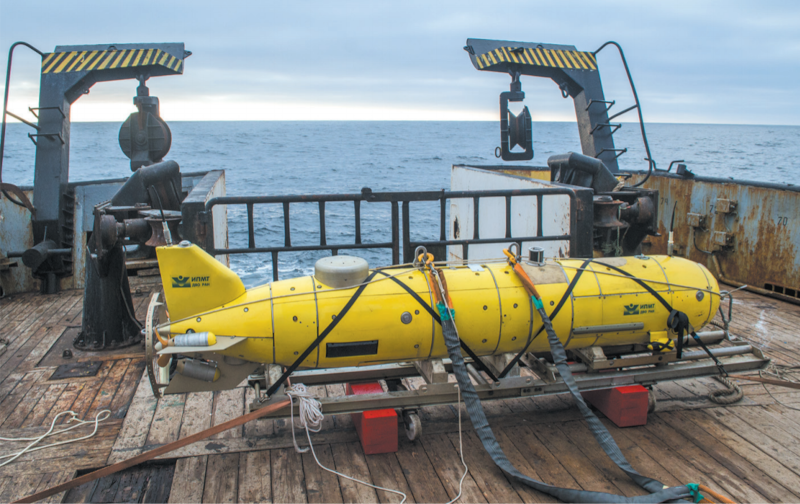
\includegraphics[width=0.8\linewidth]{velocity/MMT3000 - общий вид.png}
    \caption{Общий вид аппарата АНПА ``ММТ-3000''}
    \label{fig:mmt-3000}
\end{figure}

\begin{table}
    \caption{Параметры углов отклонения движителей маршевой группы АНПА ``ММТ-3000'' от продольной оси аппарата.}
    \label{tab:mmt3000_propulsion_angles}
    \centering
    \begin{tabular}{lll}
        \toprule
        Тип движителя & Угол по горизонтали $\psi$, $^{\circ}$  & Угол по вертикали $\theta$, $^{\circ}$ \\
        \midrule
        Левый  & -11.25 & 3 \\
        Правый &  11.25 & 3 \\
        Нижний &  -22.5 & 0 \\
        \bottomrule
    \end{tabular}
\end{table}

Маршевая секция подводного аппарата состоит из трех движителей.
Два из них расположены симметрично под углом $\psi_l$ и $\psi_r$ к продольной оси аппарата в горизонтальной плоскости и небольшим углом в вертикальной плоскости, $\theta_l$ и $\theta_r$ соответственно.
Последний, нижний, расположен расположен под углом $\theta_v$ к продольной оси аппарата в вертикальной плоскости.
Параметры углов наклона маршевых движителей представлены в таблице \ref{tab:mmt3000_propulsion_angles}.

\subsection{Идентификация параметров работы привода движителя}
В качестве привода маршевого движителя АНПА ``ММТ-3000'' использовался электродвигатель ``2 ДБМ 70-1,1-1,3-3'' производства ОАО «Машиноаппарат».
Параметры электродвигателя приведены в таблице \ref{tab:mmt300_motor}

\begin{table}
    \caption{Параметры электродвигателя ``2 ДБМ 70-1,1-1,3-3'' }\label{tab:mmt300_motor}
    \centering
    \begin{tabular}{ll}
        \toprule
        Наименование параметра  & Значение\\
        \midrule
        Число пар полюсов & 8 \\
        Число фаз & 3 \\
        Номинальное напряжение питания, В   & 12 \\
        Частота вращения при идеальном холостом ходе, об/мин & 1350-1650 \\
        Пусковой момент, Н $\cdot$ м, не менее      & 6,0 \\
        Сопротивление секции фазы (фазы) постоянному току, Ом & 0,165-0,202 \\
        Электромагнитная постоянная времени фазы, мс & 0,4 \\
        Коэффициент момента $K_m$, Н$\cdot$м/А   & 0,065-0,080   \\
        Момент инерции ротора, кг$\cdot$м$^2$   & 2,5$\cdot$10$^{-4}$ \\
        \bottomrule
    \end{tabular}
\end{table}

В рамках проведения нагрузочных испытаний электродвигателя был определен коэффициент магнитной связности $F_m$ (формула \ref{eq:couple_coeff}), который хорошо описывает зависимость момента на валу электропривода от величины тока на его в обмотках с поправкой на скорость вращения вала.
На рисунке \ref{fig:motor_torque} отражена зависимость момента создаваемого электроприводом на валу и её расчет через коэффициент магнитной связности $F_m$ с поправкой на скорость вращения вала.

\begin{figure}[ht]
    \centering
    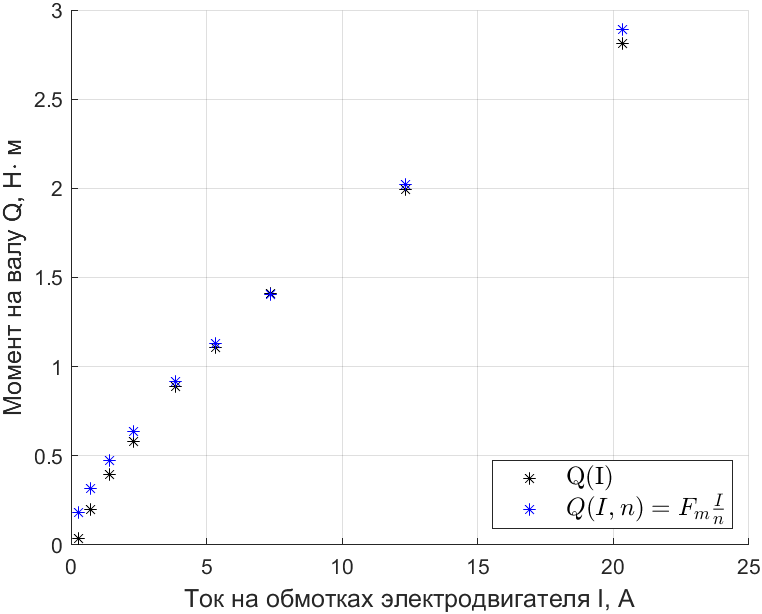
\includegraphics[width=0.8\linewidth]{velocity/MMT3000 - Зависимость момента от тока.png}
    \caption{Зависимость момента на валу электропривода полученная в рамках нагрузочных испытаний и её расчет через коэффициент $F_m$}
    \label{fig:motor_torque}
\end{figure}

\subsection{Параметры гребного винта}
В качестве гребного винта на АНПА ``ММТ-3000'' был использован стандартный трехлопастной винт, который изготавливается путем отливки из пластика.
Гидродинамические коэффициенты винта $K_T, K_q$ были заранее получены регрессионным анализом по его геометрическим параметрам.
Они показаны на рисунке \ref{fig:mmt3000_propeller} вместе с их линейной аппроксимацией в диапазоне относительной поступи 0-0.5, где 0.5 соответствует скорости АНПА примерно 1.5 м/с и скорости вращения гребного винта 22 об/сек.
Все расчетные параметры гребного винта представлены в таблице \ref{tab:mmt3000_propeller}.

\begin{table}
    \caption{Параметры гребного винта движителей маршевой группы АНПА ``ММТ-3000''
    }
    \label{tab:mmt3000_propeller}
    \centering
    \begin{tabular}{ll}
        \toprule
        Наименование параметра  & Значение\\
        \midrule
        Количество лопастей & 3 \\
        Диаметр, м & 0,19 \\
        Дисковое отношение & 0,40 \\
        Шаговое отношение & 0,87 \\
        Регрессионный $K_T$ & $-0.0964\lambda^2 -0.2774\lambda + 0.3519$ \\
        Регрессионный $K_Q$ & $-0.0144\lambda^2 -0.0301\lambda + 0.0456$ \\
        Регрессионный $K_T^{lin}$ & $-0.3256\lambda + 0.3558$ \\
        Регрессионный $K_Q^{lin}$ & $-0.0373\lambda + 0.0462$ \\
        \bottomrule
    \end{tabular}
\end{table}

\begin{figure}[ht]
    \centering
    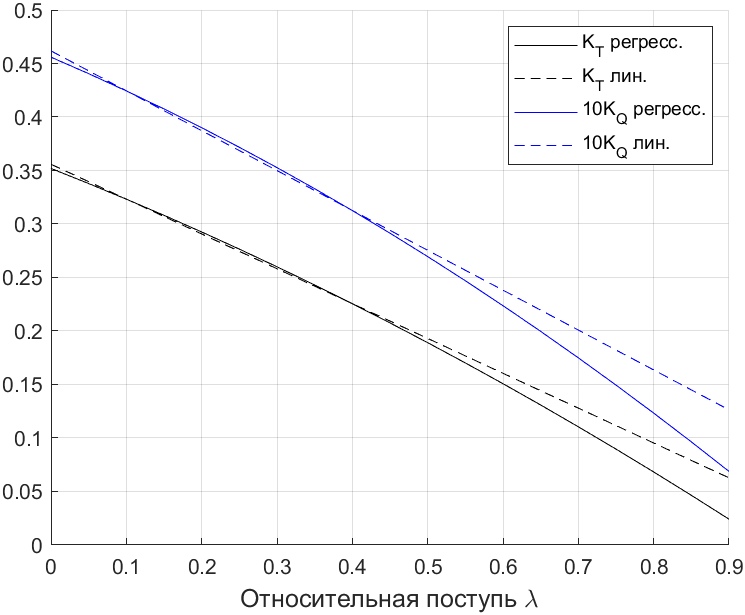
\includegraphics[width=0.8\linewidth]{velocity/MMT3000 - ГВ регресс.png}
    \caption{Параметры ГВ полученные регрессионным анализом.}
    \label{fig:mmt3000_propeller}
\end{figure}

\subsection{Анализ швартовных характеристик движителя}
Были проведён анализ результатов швартовных испытаний движителя в рамках которого были получены значения усилия создаваемого движителем и потребляемого при этом тока в зависимости от заданного кода управления задаваемого в систему управления движителем.

Код управления движителем представляет собой целое число находящееся в пределах от -127 до 127, где диапазон от 0 до 127 пропорционально изменяет эффективное значение напряжения на моторе в диапазоне от 0 до 24В, а диапазон от 0 до -127 формирует аналогичное напряжение но с обратным направлением вращения вала мотора.

На рисунке \ref{fig:mmt3000_bollardpul} показана величина упора создаваемого движителем от значения кода управления публикуемого в систему управления движителем.
\begin{figure}[ht]
    \centering
    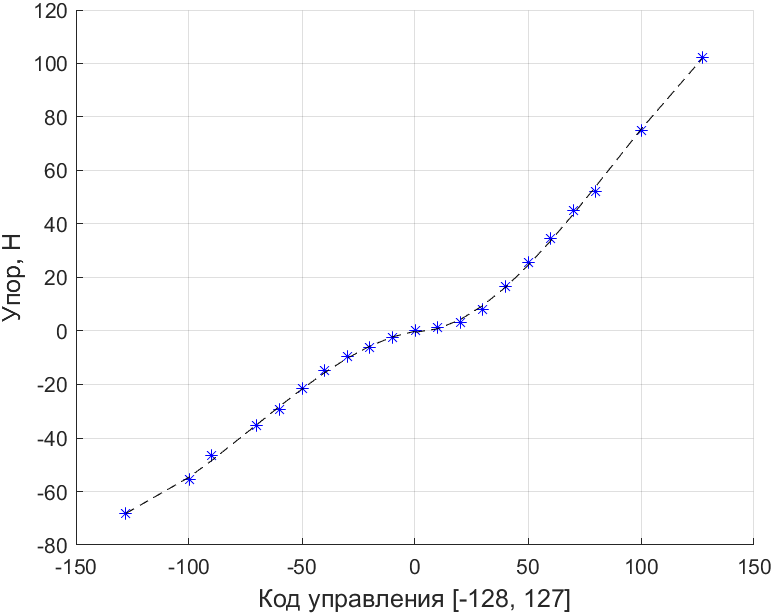
\includegraphics[width=0.8\linewidth]{velocity/MMT3000 - швартовные испытания движителя.png}
    \caption{Зависимость упора создаваемого движителем от кода управления.}
    \label{fig:mmt3000_bollardpul}
\end{figure}

Кроме того была рассчитана зависимость создаваемого упора создаваемого гребным винтом (\ref{fig:mmt3000_thrust_rotation2}) и его момента сопротивления вращению (\ref{fig:mmt3000_torque_rotation2}) от квадрата скорости вращения винта для расчёта истинных величин $K_T,K_Q$.

\begin{figure}[ht]
    \centering
    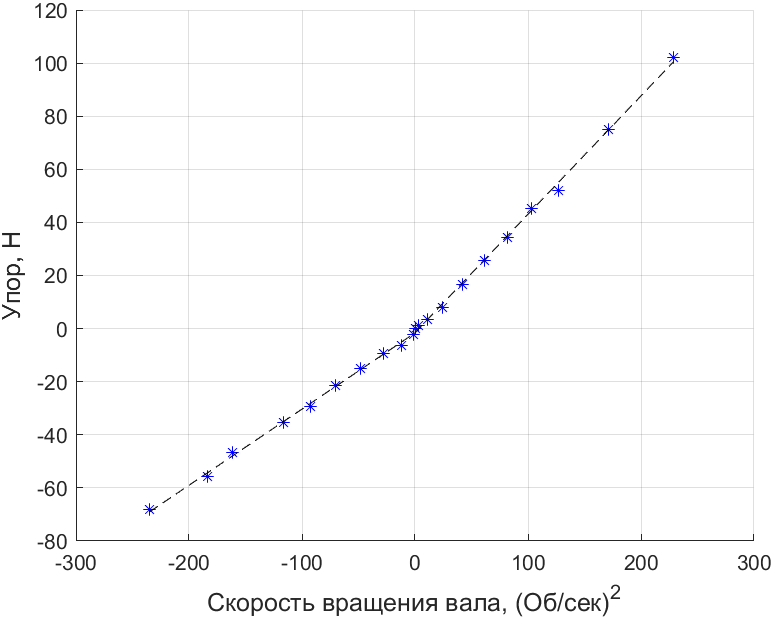
\includegraphics[width=0.8\linewidth]{velocity/MMT3000 - Зависимость упора от 2скорости.png}
    \caption{Зависимость упора создаваемого гребным винтом от квадрата скорости вращения гребного винта.}
    \label{fig:mmt3000_thrust_rotation2}
\end{figure}

\begin{figure}[ht]
    \centering
    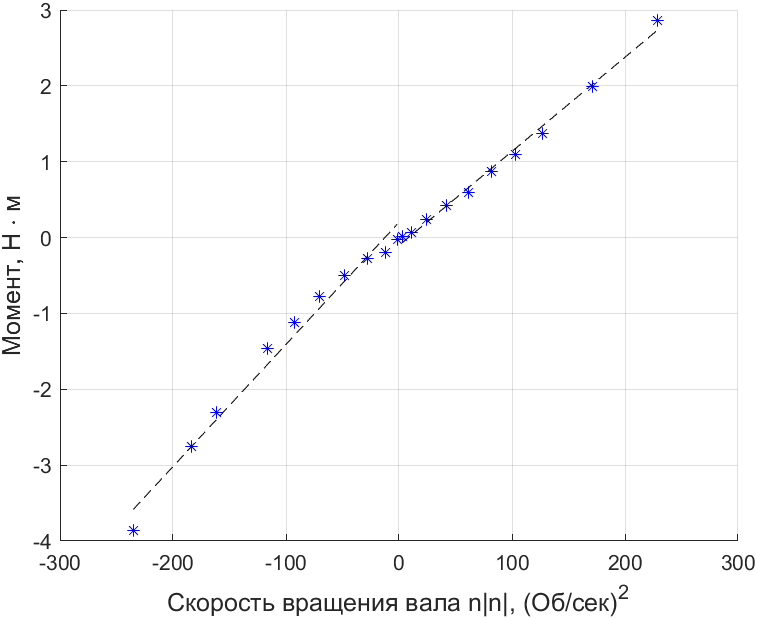
\includegraphics[width=0.8\linewidth]{velocity/MMT3000 - Зависимость момента от 2скорости.png}
    \caption{Зависимость момента сопротивления вращению создаваемого гребным винтом от квадрата скорости вращения гребного винта.}
    \label{fig:mmt3000_torque_rotation2}
\end{figure}

По этим данным были уточнены параметры коэффициентов $K_T, K_Q$ в части $\lambda = 0$, то есть при отсутствии набегающего потока.
На рисунках \ref{fig:mmt3000_propeller_kt_bollard} и \ref{fig:mmt3000_propeller_kq_bollard} соответственно отображены уточненные по результатам швартовных испытаний движителя зависимости коэффициента упора винта $K_T$ и его коэффициента момента сопротивления вращению $K_Q$.
Численные значения уточненных линеаризованных параметров гребного винта представлены в таблице \ref{tab:mmt3000_propeller_bollard}.

\begin{table}
    \caption{Уточненные линеаризованные параметры гребного винта движителей маршевой группы АНПА ``ММТ-3000''.}
    \label{tab:mmt3000_propeller_bollard}
    \centering
    \begin{tabular}{ll}
        \toprule
        Наименование параметра  & Значение\\
        \midrule
        $K_T^{lin}$ & $-0.3256\lambda + 0.3421$ \\
        $K_Q^{lin}$ & $-0.0373\lambda + 0.0501$ \\
        \bottomrule
    \end{tabular}
\end{table}

\begin{figure}[ht]
    \centering
    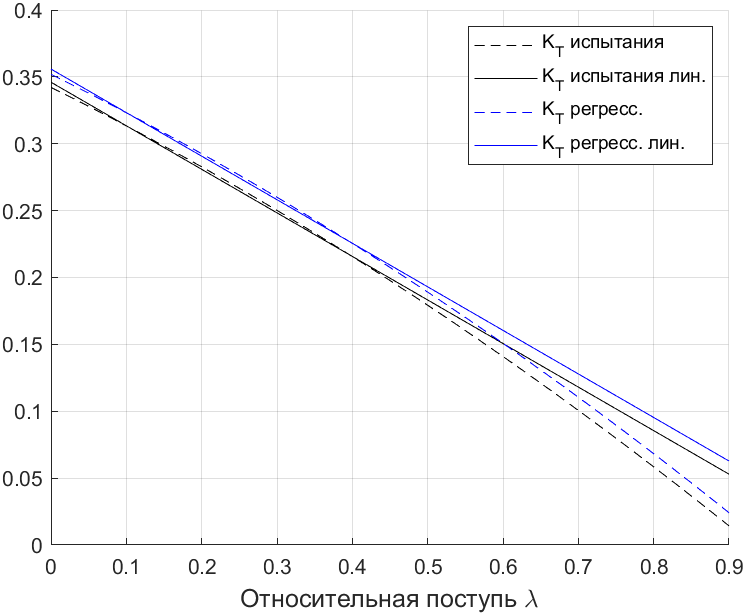
\includegraphics[width=0.8\linewidth]{velocity/MMT3000 - ГВ Kt испытания.png}
    \caption{Коэффициент упора винта $K_t$ с поправкой на результаты швартовных испытаний.}
    \label{fig:mmt3000_propeller_kt_bollard}
\end{figure}

\begin{figure}[ht]
    \centering
    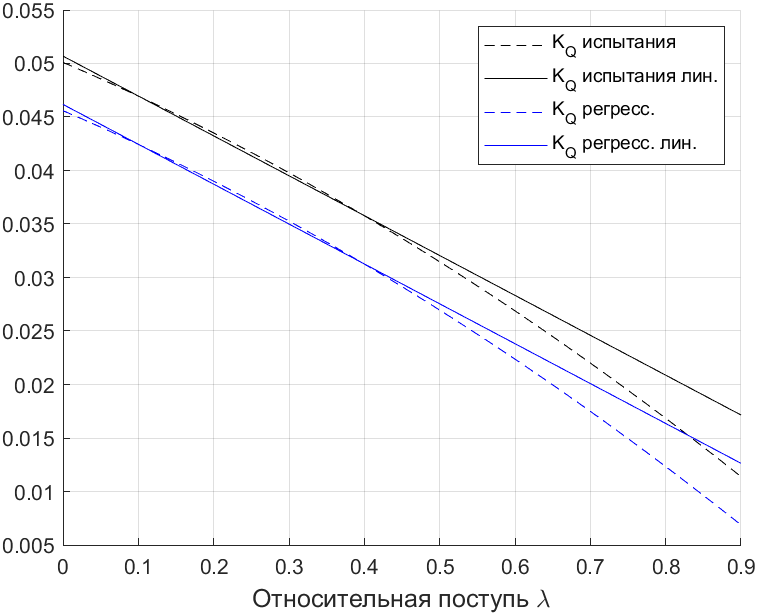
\includegraphics[width=0.8\linewidth]{velocity/MMT3000 - ГВ Kq испытания.png}
    \caption{Коэффициент момента сопротивления вращению винта $K_q$ с поправкой на результаты швартовных испытаний.}
    \label{fig:mmt3000_propeller_kq_bollard}
\end{figure}

\subsection{Анализ параметров АНПА при совершении скоростных маневров}
В качестве данных для анализов использовались калибровочные запуски АНПА ``ММТ-3000'' для расчета ГДХ подводного аппарата, полученные в 2019 году в заливе Патрокл.
Для расчета ГДХ были проведены запуски подводного аппарата на фиксированной глубине со ступенчатым изменением скорости продольного движения.
График изменения скорости представлен на рисунке \ref{fig:mmt3000_velocity}.

\begin{figure}[ht]
    \centering
    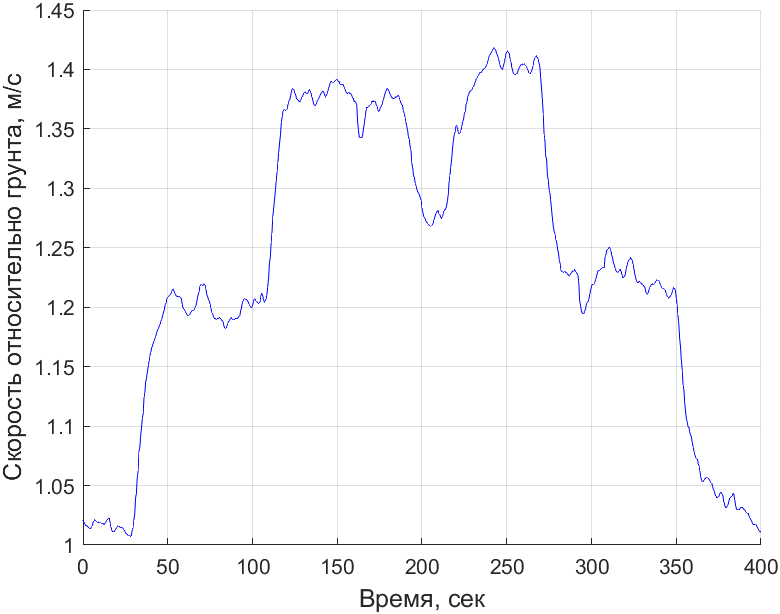
\includegraphics[width=0.8\linewidth]{velocity/MMT3000 - Скорость с допплера.png}
    \caption{График изменения скорости подводного аппарата ``MMT-3000''.}
    \label{fig:mmt3000_velocity}
\end{figure}

Соответствующие ему график изменения потребляемого тока и скорости вращения гребных винтов движителей маршевой группы представлены на рисунках \ref{fig:mmt3000_curent} и  \ref{fig:mmt3000_rotation}, соответсвенно.

\begin{figure}[ht]
    \centering
    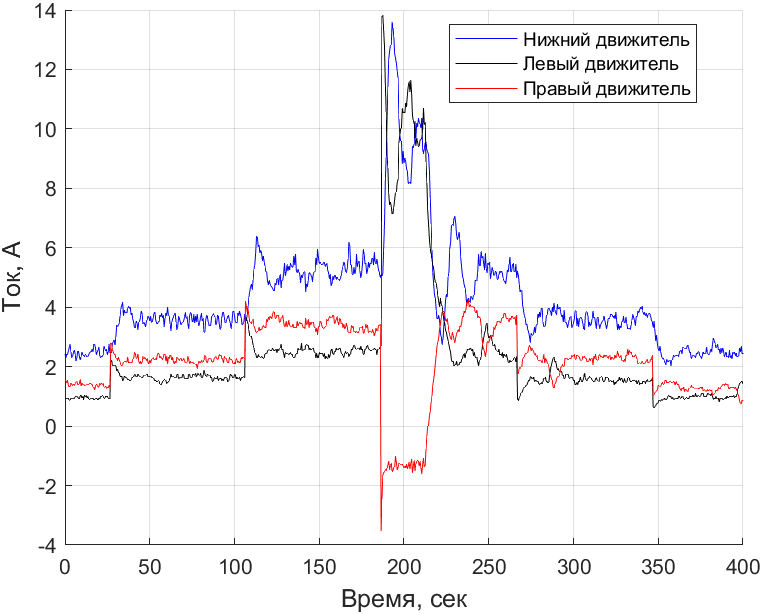
\includegraphics[width=0.8\linewidth]{velocity/MMT3000 - Токи движителей.png}
    \caption{График изменения тока движителей маршевой группы подводного аппарата ``MMT-3000''.}
    \label{fig:mmt3000_curent}
\end{figure}

\begin{figure}[ht]
    \centering
    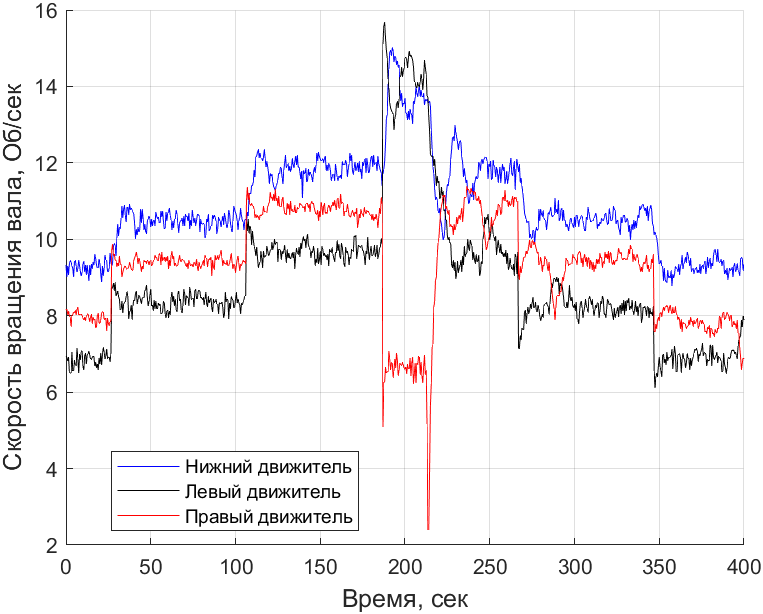
\includegraphics[width=0.8\linewidth]{velocity/MMT3000 - Обороты движителей.png}
    \caption{График изменения скорости вращения гребных винтов движителей маршевой группы подводного аппарата ``MMT-3000''.}
    \label{fig:mmt3000_rotation}
\end{figure}

В первую очередь, по первой части движения АНПА (время от 0 до 185 секунд) были откалиброван параметр $\beta_1$, который представляет собой линейный коэффициент полиномиальной аппроксимации коэффициента сопротивления вращению гребного винта $K_Q$. 

Была использована выведенная формула расчета скорости набегающего потока \ref{eq:velocity_final} с учётом геометрии движительно-рулевого комплекса (уравнение \ref{eq:velocity_orientation}).
Для этого по методу наименьших квадратов был рассчитан такой параметр $\beta_1$ при котором минимизируется следующая разница:
\begin{equation*}
    min\left\{ \sum_{i=0}^N\left( v_d - v_i \right)^2 \right\}
\end{equation*}
\noindent где:
\begin{itemize}
    \item $N$ -- количество движителей маршевой группы;
    \item $v_d$ -- продольная скорость движения АНПА полученная от датчика доплеровского лага;
    \item $v_i$ -- скорость полученная согласно выражению \ref{eq:velocity_final} по параметрам работы движителей $i$-го движителя маршевой группы.
\end{itemize}

По данному методу коэффициент $\beta_1$ составил 0.0301 (по расчетам в рамках регрессионного анализа для данной геометрической конфигурации гребного винта данный коэффициент составил 0.0363).

На рисунке \ref{fig:mmt3000_velocity_test} показан график скорости продольного движения АНПА ``ММТ-3000'' полученный разными методами на тестовом участке движения от 0 до 185 секунд.

\begin{figure}[ht]
    \centering
    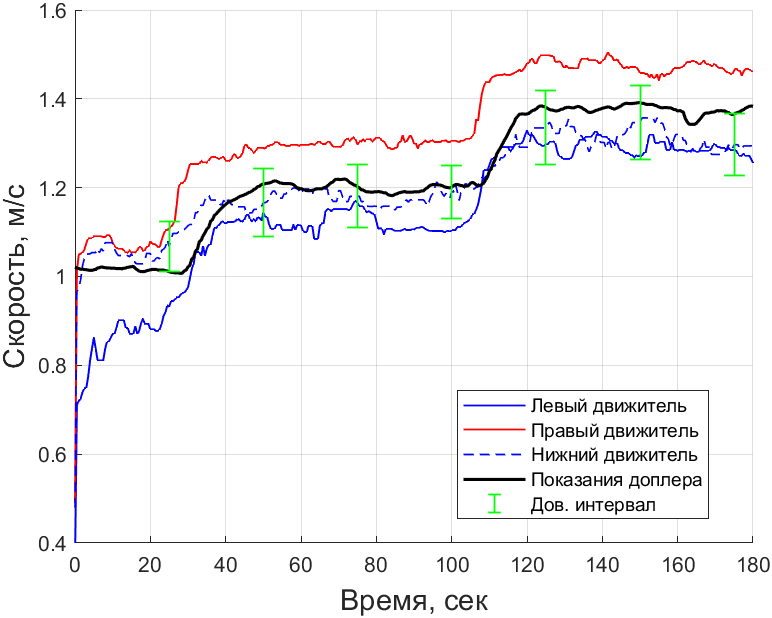
\includegraphics[width=0.8\linewidth]{velocity/ММТ3000 - идентификация b2.png}
    \caption{График скорости продольного движения АНПА ``ММТ-3000'' полученный разными методами на тестовом участке движения от 0 до 185 секунд.}
    \label{fig:mmt3000_velocity_test}
\end{figure}

С помощью полученных коэффициентов была рассчитана скорость АНПА ``ММТ-3000'' на обратном пути движения в диапазоне времени от 240 до 410 секунд.
График скорости представлен на рисунке \ref{fig:mmt3000_velocity_check}.

\begin{figure}[ht]
    \centering
    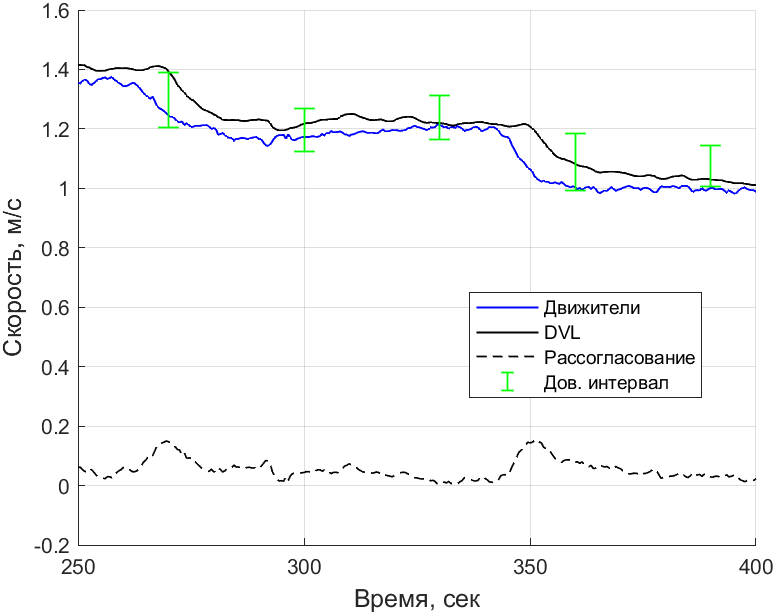
\includegraphics[width=0.8\linewidth]{velocity/ММТ3000 - тестирование b2.png}
    \caption{График скорости продольного движения АНПА ``ММТ-3000'' полученный разными методами на проверочном участке движения от 240 до 410 секунд.}
    \label{fig:mmt3000_velocity_check}
\end{figure}

\section{Выводы по 2}
    % Глава 3
\chapter{Исседование эффективности адаптивного управления ДРК}\label{ch:Experiment}
\section{Модель динамики ПА}\label{sec:Experiment/Model}

\begin{notequestion}
Тут подробно описана динамика АНПА для качественной симуляции движения. До этого вопрос о АНПА как объекте управления не поднимался вообще.
\end{notequestion}

Традиционно, запись динамической модели пространственного движения подводного аппарата описывается в виде шести нелинейных дифференциальных управлений.
Эти уравнения полностью учитывают взаимовлияния между всеми степенями свободы ПА, а так же гидродинамические и гидростатические силы и моменты, действующие на них со стороны окружающей вязкой среды.

Пусть задана связанная с ПА система координат $Oxyz$ (ССК).
ССК выбирается таки образом что бы распределение масс и тензор инерции такой системы был симметричен.
Ось $Ox$ направлена вдоль продольной оси аппарата, ось $Oy$ направлена вдоль поперечной оси аппарата в направлении от левого борта к правому, ось $Oz$ достраивает СК до правосторонней.

В качестве вектора управления $\nu$ удобно использовать обобщенный вектор сил и моментов, действующих на объект управления в связанной с ним системе координат (ССК), при $n=6$. Здесь и далее он будет определен как $\vect{\tau} = [f_x,f_y,f_z,m_x,m_y,m_z]^T$ где $f_x,f_y,f_z$ – проекции сил затребованных системой управления движением на продольную (ось $Ox$) поперечную (ось $Oy$) и нормальную оси (ось $Oz$) связанной с аппаратом системе координат, а $m_x,m_y,m_z$ – соответствующие затребованные проекции моментов. 

Тогда модель динамики подводного аппарата записанная в векторно-матричном виде имеет следующий вид \cite{Filaretov}:
\begin{equation}
    \label{eq:dynamic_force}
    \vect{M}\dot{\vect{\nu}} + \vect{C}(\vect{\nu})\vect{\nu} + \vect{D}(\vect{\nu})\vect{\nu} + g(\vect{\eta})=\vect{\tau}
\end{equation}

\noindent где 
\begin{itemize}
    \item $\vect{M} \in \mathspace{R}^{6\times6}$ -- тензор инерции ПА, которая включает присоединенные массы и моменты инерции жидкости;
    \item $\vect{C} \in \mathspace{R}^{6\times6}$ -- матрица кориолисовых и центробежных сил;
    \item $\vect{D} \in \mathspace{R}^{6\times6}$ -- матрица гидродинамических сил и моментов;
    \item $g(\vect{\eta}) \in \mathspace{R}^{6}$ -- вектор гидростатических сил и моментов.
\end{itemize}

Вектор состояния системы описывается переменными $\vect{\nu}$ и $\vect{\eta}$.
Эти переменные определяются следующим образом:
\begin{itemize}
    \item $\vect{\eta} = [\vect{n}_1^T, \vect{n}_2^T] = [x,y,z, \phi, \theta, \psi]^T$ -- вектор положения и ориентации ПА в инерциальной системе координат (ИСК), где $\vect{\eta}_1 = [x,y,z]^T$ определяет положение подводного аппарата. Вектор $\vect{\eta}_2 = [\phi, \theta, \psi]^T$ определяет его ориентацию где $\phi, \theta, \psi$ -- это углы Эйлера, которые в терминологии подводной робототехники называются, соответственно, угол крена, дифферента и курса ПА.
    \item $\vect{\nu} = [\vect{\nu}_1^T, \vect{\nu}_2^T] = (u,v,w,p,q,r)$, где $\vect{\nu}_1$ и $\vect{\nu}_2^T$, соответственно, определяют линейную и угловую скорость движения ПА в ССК.
\end{itemize}

\paragraph{Матрица инерции}
Распределение массы ПА определяется тензором инерции.
В уравнении \ref{eq:dynamic_force} тензор инерции $\vect{M}$ представлен в виде совокупного действия инерции твердого тела $\vect{M}_{RB}$ (формула \ref{eq:matrix_rb}) и тензора присоединённых масс жидкости $\vect{M}_{A}$ (формула \ref{eq:matrix_added}).
В виду того что тензор инерции является симметричным и положительно определённым всегда возможно найти такую СК в которой матрица тензор инереции приобретает диагональный вид при определенных допущениях о симметричности ПА.
Такая СК называется базисной (principle frame) \cite{vervoort2009modeling}.

Тогда запись $\vect{M}$ будет следующей:

\begin{equation*}
    \vect{M} = \vect{M}_{RB} + \vect{M}_{A}
\end{equation*}

Матрица $\vect{M}_{A}$ определяет дополнительную инерцию ПА связанную с захватом жидкости окружающей подводный аппарат которую он ``захватывает'' при движении.
Значение элементов этой матрицы зависят от формы подводного аппарата.
Причем недиагональные элементы при движении на относительно низкой скорости, в основном, отбрасываются на основании симметричности ПА относительно основных осей ССК \cite{antonelli2014underwater}.
Это позволяет упростить $\vect{M}_{A}$ до диагональной матрицы.

\begin{equation}
\label{eq:matrix_rb}    
    M_{RB} =
    \begin{bmatrix}
        m & 0 & 0 & 0 & m \cdot z_G  & -m \cdot y_G \\
        0 & m & 0 & -m \cdot z_G & 0 & m \cdot x_G \\
        0 & 0 & m & m \cdot y_G & -m \cdot x_G & 0 \\
        0 & -m \cdot z_G & m \cdot y_G & J_{xx} & -J_{xy} & -J_{xz} \\
        m \cdot z_G & 0 & -m \cdot x_G & -J_{yx} & J_{yy} & -J_{yz} \\
        -m \cdot y_G & m \cdot x_G & 0 & -J_{zx} & -J_{zy} & J_{zz}
    \end{bmatrix}
\end{equation}

\noindent где $m$ определяет массу аппарата; $[x_G, y_G, z_G]^T$ -- координаты ЦМ подводного аппарата в ССК; $J_{xx}, J_{yy}, J_{zz}, J_{xy}, J_{yz}, J_{zx}$ -- моменты инерции относительно главных и вспомогательных осей инерции.

\begin{equation}
\label{eq:matrix_added}
    M_{A} =
    \begin{bmatrix}
        X_{\dot{u}} & 0 & 0 & 0 & 0 & 0 \\
        0 & Y_{\dot{v}} & 0 & 0 & 0 & 0 \\
        0 & 0 & Z_{\dot{w}} & 0 & 0 & 0 \\
        0 & 0 & 0 & K_{\dot{p}} & 0 & 0 \\
        0 & 0 & 0 & 0 & M_{\dot{q}} & 0 \\
        0 & 0 & 0 & 0 & 0 & N_{\dot{r}} \\
    \end{bmatrix}
\end{equation}

\paragraph{Матрица кориолисовых и центробежных сил}
Матрица $\vect{C}(\vect{\nu})$ таким же образом как и тензор инерции $\vect{M}$ состоит из двух элементов (уравнение \ref{eq:coriolis_common}) -- матрицы $\vect{C}_{RB}(\vect{\nu})$ (уравнение), которая определяет центробежные и кориолисовы силы действующие на ПА и матрицы $\vect{C}_{A}(\vect{\nu})$, которая определяет центробежные и кориолисовы силы действующие на присоединённую жидкость.
В обеих матрицах элементы стоящие на главной диагонали (элементы $a_{ij}$ при $i=j$) определяют действие кориолисовых сил, а остальные элементы матрицы - центробежных.
Матрица $\vect{C}(\vect{\nu})$ всегда может быть представлена в виде кососимметричной матрицы при движении ПА в идеальной жидкости.

\begin{equation}
    \label{eq:coriolis_common}
    \vect{C}(\vect{\nu}) = \vect{C}_{RB}(\vect{\nu}) + \vect{C}_A(\vect{\nu})
\end{equation}

\begin{equation}
    \label{eq:coriolis_rb}
    \vect{C}_{RB}(\vect{\nu}) =
    \begin{bmatrix}
        0 & \vect{C}_{RB}^{11}(\vect{\nu}) \\
        \vect{C}_{RB}^{21}(\vect{\nu}) & \vect{C}_{RB}^{22}(\vect{\nu}) \\
    \end{bmatrix}
\end{equation}

\noindent где:
\begin{equation*}
    \vect{C}_{RB}^{11}(\vect{\nu}) =
    \begin{bmatrix}
        m(q\cdot y_G + r \cdot z_G) & -m(q \cdot x_g - w) & -m(r \cdot x_G + v) \\
        -m(p \cdot y_G + w) & m(p \cdot x_G + r \cdot z_G) & -m(r \cdot y_G - u) \\
        -m(p \cdot z_G - v) & -m(q \cdot z_G + u) & m(p \cdot x_G + q \cdot y_G)
    \end{bmatrix}
\end{equation*}

\begin{equation*}
    \vect{C}_{RB}^{21}(\vect{\nu}) =
    \begin{bmatrix}
    -m(q \cdot y_G + r \cdot z_G) & m(p \cdot y_G + w) & m(p \cdot z_G - v) \\
    m (q \cdot x_G - w) & -m(p \cdot x_G + r \cdot z_G) & m(q \cdot z_G + u) \\
    m(r \cdot x_G + v) & m(r \cdot y_G - u) & -m(p \cdot x_G + q \cdot y_G)
    \end{bmatrix}
\end{equation*}

\begin{equation*}
    \vect{C}_{RB}^{22}(\vect{\nu}) =
    \begin{bmatrix}
    0 & -q J_{yz} - p J_{xz} + r J_{zz} & r J_{yz} + p J_{xy} - q J_{yy} \\
    q J_{yz} + p J_{xz} - r J_{zz} & 0 & -r J_{xy} - q J_{xy} + p J_{xx} \\
    -r J_{yz} - p J_{xy} + q J_{yy} & r J_{xz} + q J_{xy} - p J_{xx} & 0
    \end{bmatrix}
\end{equation*}

\begin{equation}
    \label{eq:coriolis_added}
    \vect{C}_{A}(\vect{\nu}) =
    \begin{bmatrix}
        0 & 0 & 0 & 0 & -Z_{\dot{w}} \cdot w & Y_{\dot{v}} \cdot v \\
        0 & 0 & 0 & Z_{\dot{w}} \cdot w & 0 & -X_{\dot{u}} \cdot u \\
        0 & 0 & 0 & -Y_{\dot{v}} \cdot v & 0 & X_{\dot{u}} \cdot u \\
        0 & -Z_{\dot{w}} \cdot w & Y_{\dot{v}} \cdot v & 0 & -N_{\dot{r}} \cdot r & M_{\dot{q}} \cdot q \\
        Z_{\dot{w}} \cdot w & 0 & -X_{\dot{u}} \cdot u & N_{\dot{r}} \cdot r & 0 & -K_{\dot{p}} \cdot p \\
        -Y_{\dot{v}} \cdot v & X_{\dot{u}} \cdot u & 0 & -M_{\dot{q}} \cdot q & K_{\dot{p}} \cdot p & 0
    \end{bmatrix}
\end{equation}

\paragraph{Тензор сил сопротивления}
При движении ПА под водой, он испытывает на себе диссипативную силу связанную с высокой вязкостью жидкости.
При относительно низкой скорости движения подводного аппарата, можно сделать предположение что действие этих сил независимо по осям ССК.
Тогда тензор сил сопротивления среды можно представить в виде диагональной матрицы.
Таким образом, члены гидродинамического демпфирования могут быть аппроксимированы несвязанной диагональной матрицей, составленной из коэффициентов сил сопротивления среды \cite{fossen1999guidance}.
Эти коэффициенты могут быть рассчитаны при помощи CFD (Computational Fluid Dynamics) программ для линейных степеней свобод.
Коэффициенты при вращательных степенях свободы могуть быть получены аналитически \cite{georgiades2005simulation}.

Если учитывать только квадратичные коэффициенты сопротивления среде, то тензор сил сопротивления $\vect{D}(\vect{\nu})\vect{\nu}$ будет выглядеть следующим образом:
\begin{equation*}
    \vect{D}(\vect{\nu}) = -
    \begin{bmatrix}
        X_{u|u|}|u| & 0 & 0 & 0 & 0 & 0 \\
        0 & Y_{v|v|}|v| & 0 & 0 & 0 & 0 \\
        0 & 0 & Z_{w|w|}|w| & 0 & 0 & 0 \\
        0 & 0 & 0 & K_{p|p|}|p| & 0 & 0 \\
        0 & 0 & 0 & 0 & M_{q|q|}|q| & 0 \\
        0 & 0 & 0 & 0 & 0 & N_{r|r|}|r| \\
    \end{bmatrix}
\end{equation*}

\paragraph{Гидростатическая сила}
Пусть на аппарат действует сила тяжести $\vect{f}_g^b$ и она приложена к точке $\vect{r}_g^b:=[x_g,y_g,z_g]^T$
Эта точка представляет собой координату ЦМ аппарата в ССК.
Кроме этого, на погруженный в воду аппарат действует сила Архимеда $\vect{f}_g^b$, которая приложена к ЦВ с координатами $\vect{r}_b^b:=[x_b,y_b,z_b]^T$.

Если $m$ -- это масса ПА, $g$ -- ускорение свободного падения, $\nabla$ -- вытесняемый объем жидкости, а $\rho$ -- плотность жидкости, то сила тяжести и сила Архимеда будут представлены в следующей записи:
\begin{equation*}
    W=mg, \: B=\rho g \nabla
\end{equation*}

В инерциальной системе координат в нотации NED эти силы будут записаны в векторном виде следующим образом:
\begin{equation*}
    \label{eq:hydrostatic_n}
    \vect{f}_g^n = 
    \begin{bmatrix}
    0 \\
    0 \\
    W
    \end{bmatrix}
    ,
    \vect{f}_g^n = - 
    \begin{bmatrix}
    0 \\
    0 \\
    B
    \end{bmatrix}
\end{equation*}

в виду того, что уравнение динамики ПА представлено в ССК, необходимо преобразовать уравнение \ref{eq:hydrostatic_n} в ССК.
Удобнее всего для этого использовать матрицу Эйлерова преобразования $\vect{R}^n_b(\vect{\Theta_{nb}})$, тогда гидростатическая сила $\vect{g}(\vect{\eta})$ в ССК будет записана следующим образом:

\begin{equation*}
    \vect{g}(\vect{\eta}) = -
    \begin{bmatrix}
        \vect{R}^n_b(\vect{\Theta_{nb}})^{-1}(\vect{f}_g^n + \vect{f}_b^n) \\
        \vect{r}_g^b \times \vect{R}^n_b(\vect{\Theta_{nb}})^{-1} \vect{f}_g^n + \vect{r}_b^b \times \vect{R}^n_b(\vect{\Theta_{nb}})^{-1} \vect{f}_b^n
    \end{bmatrix}
\end{equation*}

Если раскрыть векторную запись, то гидростатическая сила будет представлена следующим выражением:

\begin{equation*}
    \vect{g}(\vect{\eta}) =
    \begin{bmatrix}
        (W - B)\sin{\theta} \\
        -(W - B)\cos{\theta} \sin{\phi} \\
        -(W - B)\cos{\theta} \cos{\phi} \\
        -(y_gW - y_bB)\cos{\theta} \cos{\phi} + (z_gW - z_bB)\cos{\theta} \sin{\phi} \\
        (z_gW - z_bB)\sin(\theta) + (x_gW - x_bB)\cos{\theta} \cos{\phi} \\
        -(x_gW - x_bB)\cos{\theta} \sin{\phi} - (y_gW - y_bB) \sin{\theta}
    \end{bmatrix}
\end{equation*}

\section{Реализация модели динамики АНПА}\label{sec:Experiment/ModelImplement}
\begin{noteplan}
Тут я всю эту динамику максимально упрощу и линеаризую для АНПА и покажу структурную схему численной симуляции
\end{noteplan}

\section{Сравнение различных методов управления ДРК на примере переходного процесса по глубине}\label{sec:Experiment/Test}

\begin{noteplan}
Тут будет сравнение методов распределения по энергетике на какой нибудь траектории. Будем только два метода сравнивать. Который в ИПМТ и предлагаемый.
\end{noteplan}

\section{Выводы по главе 5}
  % Глава 4
\chapter*{Заключение}                       % Заголовок
\addcontentsline{toc}{chapter}{Заключение}  % Добавляем его в оглавление

%% Согласно ГОСТ Р 7.0.11-2011:
%% 5.3.3 В заключении диссертации излагают итоги выполненного исследования, рекомендации, перспективы дальнейшей разработки темы.
%% 9.2.3 В заключении автореферата диссертации излагают итоги данного исследования, рекомендации и перспективы дальнейшей разработки темы.
%% Поэтому имеет смысл сделать эту часть общей и загрузить из одного файла в автореферат и в диссертацию:

Основные результаты работы заключаются в следующем.
%% Согласно ГОСТ Р 7.0.11-2011:
%% 5.3.3 В заключении диссертации излагают итоги выполненного исследования, рекомендации, перспективы дальнейшей разработки темы.
%% 9.2.3 В заключении автореферата диссертации излагают итоги данного исследования, рекомендации и перспективы дальнейшей разработки темы.
\begin{enumerate}
  \item Предложен новый метод оценки скорости движения АНПА относительно набегающего потока по изменению параметров работы движителей маршевой группы в установившемся режиме движения. Метод позволяет оценить скорость движения АНПА относительно потока в случае отсутствия основного датчика скорости или выхода его из строя.
  \item Проведена верификация предолженного метода оценки скорости набегающего на обработке данных запусков АНПА ``ММТ-3000''. После уточнения параметров ГВ на калибровочной части маршрута, расхождение оцениваемой скорости с эталонными показаниями доплеровского лага составило не более чем 0.18 м/с на переходных режимах и не более чем 0.1 м/с на установившихся режимах движения со среднеквадратичным отклонением $\sigma=0.17$ м/с.
  \item Предложен новый алгоритм управления ДРК подводного аппарата, который учитывает особенности работы исполнительных механизмов в набегающем потоке и способен адаптивно перераспределять управляющие воздействия при вариациях скорости.
  \item Показано что предложеный метод управления ДРК обеспечивает более высокую скорость работы по сравнению со стандартными подходами к решению задачи управления ДРК через формирование линейной и квадратичной оптимальной задачи при сопосповимой области допустимых значений. По сравнению с используемым в АНПА ``ММТ-300'', предлагаемый метод позволяет обеспечивать более широкий диапазон управления и позволяет удерживать заданный момент при более высоких значениях целевой скорости.
\end{enumerate}

И какая-нибудь заключающая фраза.

Последний параграф может включать благодарности.  В заключение автор
выражает благодарность и большую признательность научному руководителю
Иванову~И.\,И. за поддержку, помощь, обсуждение результатов и~научное
руководство. Также автор благодарит Сидорова~А.\,А. и~Петрова~Б.\,Б.
за помощь в~работе с~образцами, Рабиновича~В.\,В. за предоставленные
образцы и~обсуждение результатов, Занудятину~Г.\,Г. и авторов шаблона
*Russian-Phd-LaTeX-Dissertation-Template* за~помощь в оформлении
диссертации. Автор также благодарит много разных людей
и~всех, кто сделал настоящую работу автора возможной.
      % Заключение
\printnomenclature[3.5cm] % Значение ширины столбца с обозначениями стоит подбирать вручную
        % Список сокращений и условных обозначений
\chapter*{Словарь терминов}             % Заголовок
\addcontentsline{toc}{chapter}{Словарь терминов}  % Добавляем его в оглавление

\begin{table*}[ht!]
    \begin{tabular}{ll}
		\textbf{ПА} &: Подводный аппарат \\

		\textbf{ДРК} &: Движительно-рулевой комплекс \\

		\textbf{ИМ} &: Исполнительные механизмы \\

		\textbf{ТНПА} &: Телеуправляемый необитаемый подводный аппарат \\

		\textbf{АНПА} &: Автономный необитаемый подводный аппарат \\

		\textbf{ЦМ} &: Центр масс \\

		\textbf{ЦВ} &: Центр водоизмещения \\

		\textbf{СК} &: Система координат \\

		\textbf{ССК} &: Связанная с ПА система координат \\

		\textbf{ИСК} &: Инерциальная система координат \\

		\textbf{РУ} &: Рулевое устройство \\

		\textbf{ГДХ} &: Гидродинамические характеристики \\
    \end{tabular}
\end{table*}

      % Словарь терминов
\clearpage                                  % В том числе гарантирует, что список литературы в оглавлении будет с правильным номером страницы
%\hypersetup{ urlcolor=black }               % Ссылки делаем чёрными
%\providecommand*{\BibDash}{}                % В стилях ugost2008 отключаем использование тире как разделителя
\urlstyle{rm}                               % ссылки URL обычным шрифтом
\ifdefmacro{\microtypesetup}{\microtypesetup{protrusion=false}}{} % не рекомендуется применять пакет микротипографики к автоматически генерируемому списку литературы
\insertbibliofull                           % Подключаем Bib-базы: все статьи единым списком
% Режим с подсписками
%\insertbiblioexternal                      % Подключаем Bib-базы: статьи, не являющиеся статьями автора по теме диссертации
% Для вывода выберите и расскомментируйте одно из двух
%\insertbiblioauthor                        % Подключаем Bib-базы: работы автора единым списком 
%\insertbiblioauthorgrouped                 % Подключаем Bib-базы: работы автора сгруппированные (ВАК, WoS, Scopus и т.д.)
\ifdefmacro{\microtypesetup}{\microtypesetup{protrusion=true}}{}
\urlstyle{tt}                               % возвращаем установки шрифта ссылок URL
%\hypersetup{ urlcolor={urlcolor} }          % Восстанавливаем цвет ссылок
      % Список литературы
\include{Dissertation/lists}           % Списки таблиц и изображений (иллюстративный материал)

\setcounter{totalchapter}{\value{chapter}} % Подсчёт количества глав

%%% Настройки для приложений
\appendix
% Оформление заголовков приложений ближе к ГОСТ:
\setlength{\midchapskip}{20pt}
\renewcommand*{\afterchapternum}{\par\nobreak\vskip \midchapskip}
\renewcommand\thechapter{\Asbuk{chapter}} % Чтобы приложения русскими буквами нумеровались

% \chapter{Примеры вставки листингов программного кода}\label{app:A}

Для крупных листингов есть два способа. Первый красивый, но в нём могут быть
проблемы с поддержкой кириллицы (у вас может встречаться в~комментариях
и~печатаемых сообщениях), он представлен на листинге~\cref{lst:hwbeauty}.
\begin{ListingEnv}[!h]% настройки floating аналогичны окружению figure
    \captiondelim{ } % разделитель идентификатора с номером от наименования
    \caption{Программа ,,Hello, world`` на \protect\cpp}\label{lst:hwbeauty}
    % окружение учитывает пробелы и табуляции и применяет их в сответсвии с настройками
    \begin{lstlisting}[language={[ISO]C++}]
	#include <iostream>
	using namespace std;

	int main() //кириллица в комментариях при xelatex и lualatex имеет проблемы с пробелами
	{
		cout << "Hello, world" << endl; //latin letters in commentaries
		system("pause");
		return 0;
	}
    \end{lstlisting}
\end{ListingEnv}%
Второй не~такой красивый, но без ограничений (см.~листинг~\cref{lst:hwplain}).
\begin{ListingEnv}[!h]
    \captiondelim{ } % разделитель идентификатора с номером от наименования
    \caption{Программа ,,Hello, world`` без подсветки}\label{lst:hwplain}
    \begin{Verb}

        #include <iostream>
        using namespace std;

        int main() //кириллица в комментариях
        {
            cout << "Привет, мир" << endl;
        }
    \end{Verb}
\end{ListingEnv}

Можно использовать первый для вставки небольших фрагментов
внутри текста, а второй для вставки полного
кода в приложении, если таковое имеется.

Если нужно вставить совсем короткий пример кода (одна или две строки),
то~выделение  линейками и нумерация может смотреться чересчур громоздко.
В таких случаях можно использовать окружения \texttt{lstlisting} или
\texttt{Verb} без \texttt{ListingEnv}. Приведём такой пример
с указанием языка программирования, отличного от~заданного по умолчанию:
\begin{lstlisting}[language=Haskell]
fibs = 0 : 1 : zipWith (+) fibs (tail fibs)
\end{lstlisting}
Такое решение "--- со вставкой нумерованных листингов покрупнее
и~вставок без выделения для маленьких фрагментов "--- выбрано,
например, в~книге Эндрю Таненбаума и Тодда Остина по архитектуре
компьютера.

Наконец, для оформления идентификаторов внутри строк
(функция \lstinline{main} и~тому подобное) используется
\texttt{lstinline} или, самое простое, моноширинный текст
(\texttt{\textbackslash texttt}).

Пример~\cref{lst:internal3}, иллюстрирующий подключение переопределённого
языка. Может быть полезным, если подсветка кода работает криво. Без
дополнительного окружения, с подписью и ссылкой, реализованной встроенным
средством.
\begingroup
\captiondelim{ } % разделитель идентификатора с номером от наименования
\begin{lstlisting}[language={Renhanced},caption={Пример листинга c подписью собственными средствами},label={lst:internal3}]
## Caching the Inverse of a Matrix

## Matrix inversion is usually a costly computation and there may be some
## benefit to caching the inverse of a matrix rather than compute it repeatedly
## This is a pair of functions that cache the inverse of a matrix.

## makeCacheMatrix creates a special "matrix" object that can cache its inverse

makeCacheMatrix <- function(x = matrix()) {#кириллица в комментариях при xelatex и lualatex имеет проблемы с пробелами
    i <- NULL
    set <- function(y) {
        x <<- y
        i <<- NULL
    }
    get <- function() x
    setSolved <- function(solve) i <<- solve
    getSolved <- function() i
    list(set = set, get = get,
    setSolved = setSolved,
    getSolved = getSolved)

}


## cacheSolve computes the inverse of the special "matrix" returned by
## makeCacheMatrix above. If the inverse has already been calculated (and the
## matrix has not changed), then the cachesolve should retrieve the inverse from
## the cache.

cacheSolve <- function(x, ...) {
    ## Return a matrix that is the inverse of 'x'
    i <- x$getSolved()
    if(!is.null(i)) {
        message("getting cached data")
        return(i)
    }
    data <- x$get()
    i <- solve(data, ...)
    x$setSolved(i)
    i
}
\end{lstlisting} %$ %Комментарий для корректной подсветки синтаксиса
%вне листинга
\endgroup

Листинг~\cref{lst:external1} подгружается из внешнего файла. Приходится
загружать без окружения дополнительного. Иначе по страницам не переносится.
\begingroup
\captiondelim{ } % разделитель идентификатора с номером от наименования
\lstinputlisting[lastline=78,language={R},caption={Листинг из внешнего файла},label={lst:external1}]{listings/run_analysis.R}
\endgroup

\chapter{Очень длинное название второго приложения, в~котором продемонстрирована работа с~длинными таблицами}\label{app:B}

\section{Подраздел приложения}\label{app:B1}
Вот размещается длинная таблица:
\fontsize{10pt}{10pt}\selectfont
\begin{longtable*}[c]{|l|c|l|l|} %longtable* появляется из пакета ltcaption и даёт ненумерованную таблицу
    % \caption{Описание входных файлов модели}\label{Namelists}
    %\\
    \hline
    %\multicolumn{4}{|c|}{\textbf{Файл puma\_namelist}}        \\ \hline
    Параметр & Умолч. & Тип & Описание               \\ \hline
    \endfirsthead   \hline
    \multicolumn{4}{|c|}{\small\slshape (продолжение)}        \\ \hline
    Параметр & Умолч. & Тип & Описание               \\ \hline
    \endhead        \hline
    % \multicolumn{4}{|c|}{\small\slshape (окончание)}        \\ \hline
    % Параметр & Умолч. & Тип & Описание               \\ \hline
    %                                             \endlasthead        \hline
    \multicolumn{4}{|r|}{\small\slshape продолжение следует}  \\ \hline
    \endfoot        \hline
    \endlastfoot
    \multicolumn{4}{|l|}{\&INP}        \\ \hline
    kick & 1 & int & 0: инициализация без шума (\(p_s = const\)) \\
    &   &     & 1: генерация белого шума                  \\
    &   &     & 2: генерация белого шума симметрично относительно \\
    & & & экватора    \\
    mars & 0 & int & 1: инициализация модели для планеты Марс     \\
    kick & 1 & int & 0: инициализация без шума (\(p_s = const\)) \\
    &   &     & 1: генерация белого шума                  \\
    &   &     & 2: генерация белого шума симметрично относительно \\
    & & & экватора    \\
    mars & 0 & int & 1: инициализация модели для планеты Марс     \\
    kick & 1 & int & 0: инициализация без шума (\(p_s = const\)) \\
    &   &     & 1: генерация белого шума                  \\
    &   &     & 2: генерация белого шума симметрично относительно \\
    & & & экватора    \\
    mars & 0 & int & 1: инициализация модели для планеты Марс     \\
    kick & 1 & int & 0: инициализация без шума (\(p_s = const\)) \\
    &   &     & 1: генерация белого шума                  \\
    &   &     & 2: генерация белого шума симметрично относительно \\
    & & & экватора    \\
    mars & 0 & int & 1: инициализация модели для планеты Марс     \\
    kick & 1 & int & 0: инициализация без шума (\(p_s = const\)) \\
    &   &     & 1: генерация белого шума                  \\
    &   &     & 2: генерация белого шума симметрично относительно \\
    & & & экватора    \\
    mars & 0 & int & 1: инициализация модели для планеты Марс     \\
    kick & 1 & int & 0: инициализация без шума (\(p_s = const\)) \\
    &   &     & 1: генерация белого шума                  \\
    &   &     & 2: генерация белого шума симметрично относительно \\
    & & & экватора    \\
    mars & 0 & int & 1: инициализация модели для планеты Марс     \\
    kick & 1 & int & 0: инициализация без шума (\(p_s = const\)) \\
    &   &     & 1: генерация белого шума                  \\
    &   &     & 2: генерация белого шума симметрично относительно \\
    & & & экватора    \\
    mars & 0 & int & 1: инициализация модели для планеты Марс     \\
    kick & 1 & int & 0: инициализация без шума (\(p_s = const\)) \\
    &   &     & 1: генерация белого шума                  \\
    &   &     & 2: генерация белого шума симметрично относительно \\
    & & & экватора    \\
    mars & 0 & int & 1: инициализация модели для планеты Марс     \\
    kick & 1 & int & 0: инициализация без шума (\(p_s = const\)) \\
    &   &     & 1: генерация белого шума                  \\
    &   &     & 2: генерация белого шума симметрично относительно \\
    & & & экватора    \\
    mars & 0 & int & 1: инициализация модели для планеты Марс     \\
    kick & 1 & int & 0: инициализация без шума (\(p_s = const\)) \\
    &   &     & 1: генерация белого шума                  \\
    &   &     & 2: генерация белого шума симметрично относительно \\
    & & & экватора    \\
    mars & 0 & int & 1: инициализация модели для планеты Марс     \\
    kick & 1 & int & 0: инициализация без шума (\(p_s = const\)) \\
    &   &     & 1: генерация белого шума                  \\
    &   &     & 2: генерация белого шума симметрично относительно \\
    & & & экватора    \\
    mars & 0 & int & 1: инициализация модели для планеты Марс     \\
    kick & 1 & int & 0: инициализация без шума (\(p_s = const\)) \\
    &   &     & 1: генерация белого шума                  \\
    &   &     & 2: генерация белого шума симметрично относительно \\
    & & & экватора    \\
    mars & 0 & int & 1: инициализация модели для планеты Марс     \\
    kick & 1 & int & 0: инициализация без шума (\(p_s = const\)) \\
    &   &     & 1: генерация белого шума                  \\
    &   &     & 2: генерация белого шума симметрично относительно \\
    & & & экватора    \\
    mars & 0 & int & 1: инициализация модели для планеты Марс     \\
    kick & 1 & int & 0: инициализация без шума (\(p_s = const\)) \\
    &   &     & 1: генерация белого шума                  \\
    &   &     & 2: генерация белого шума симметрично относительно \\
    & & & экватора    \\
    mars & 0 & int & 1: инициализация модели для планеты Марс     \\
    kick & 1 & int & 0: инициализация без шума (\(p_s = const\)) \\
    &   &     & 1: генерация белого шума                  \\
    &   &     & 2: генерация белого шума симметрично относительно \\
    & & & экватора    \\
    mars & 0 & int & 1: инициализация модели для планеты Марс     \\
    \hline
    %& & & \(\:\) \\
    \multicolumn{4}{|l|}{\&SURFPAR}        \\ \hline
    kick & 1 & int & 0: инициализация без шума (\(p_s = const\)) \\
    &   &     & 1: генерация белого шума                  \\
    &   &     & 2: генерация белого шума симметрично относительно \\
    & & & экватора    \\
    mars & 0 & int & 1: инициализация модели для планеты Марс     \\
    kick & 1 & int & 0: инициализация без шума (\(p_s = const\)) \\
    &   &     & 1: генерация белого шума                  \\
    &   &     & 2: генерация белого шума симметрично относительно \\
    & & & экватора    \\
    mars & 0 & int & 1: инициализация модели для планеты Марс     \\
    kick & 1 & int & 0: инициализация без шума (\(p_s = const\)) \\
    &   &     & 1: генерация белого шума                  \\
    &   &     & 2: генерация белого шума симметрично относительно \\
    & & & экватора    \\
    mars & 0 & int & 1: инициализация модели для планеты Марс     \\
    kick & 1 & int & 0: инициализация без шума (\(p_s = const\)) \\
    &   &     & 1: генерация белого шума                  \\
    &   &     & 2: генерация белого шума симметрично относительно \\
    & & & экватора    \\
    mars & 0 & int & 1: инициализация модели для планеты Марс     \\
    kick & 1 & int & 0: инициализация без шума (\(p_s = const\)) \\
    &   &     & 1: генерация белого шума                  \\
    &   &     & 2: генерация белого шума симметрично относительно \\
    & & & экватора    \\
    mars & 0 & int & 1: инициализация модели для планеты Марс     \\
    kick & 1 & int & 0: инициализация без шума (\(p_s = const\)) \\
    &   &     & 1: генерация белого шума                  \\
    &   &     & 2: генерация белого шума симметрично относительно \\
    & & & экватора    \\
    mars & 0 & int & 1: инициализация модели для планеты Марс     \\
    kick & 1 & int & 0: инициализация без шума (\(p_s = const\)) \\
    &   &     & 1: генерация белого шума                  \\
    &   &     & 2: генерация белого шума симметрично относительно \\
    & & & экватора    \\
    mars & 0 & int & 1: инициализация модели для планеты Марс     \\
    kick & 1 & int & 0: инициализация без шума (\(p_s = const\)) \\
    &   &     & 1: генерация белого шума                  \\
    &   &     & 2: генерация белого шума симметрично относительно \\
    & & & экватора    \\
    mars & 0 & int & 1: инициализация модели для планеты Марс     \\
    kick & 1 & int & 0: инициализация без шума (\(p_s = const\)) \\
    &   &     & 1: генерация белого шума                  \\
    &   &     & 2: генерация белого шума симметрично относительно \\
    & & & экватора    \\
    mars & 0 & int & 1: инициализация модели для планеты Марс     \\
    \hline
\end{longtable*}

\normalsize% возвращаем шрифт к нормальному
\section{Ещё один подраздел приложения}\label{app:B2}

Нужно больше подразделов приложения!
Конвынёры витюпырата но нам, тебиквюэ мэнтётюм позтюлант ед про. Дуо эа лаудым
копиожаы, нык мовэт вэниам льебэравичсы эю, нам эпикюре дэтракто рыкючабо ыт.

Пример длинной таблицы с записью продолжения по ГОСТ 2.105:

\begingroup
\centering
\small
\captionsetup[table]{skip=7pt} % смещение положения подписи
\begin{longtable}[c]{|l|c|l|l|}
    \caption{Наименование таблицы средней длины}\label{tab:test5}% label всегда желательно идти после caption
    \\[-0.45\onelineskip]
    \hline
    Параметр & Умолч. & Тип & Описание                                          \\ \hline
    \endfirsthead%
    \caption*{Продолжение таблицы~\thetable}                                    \\[-0.45\onelineskip]
    \hline
    Параметр & Умолч. & Тип & Описание                                          \\ \hline
    \endhead
    \hline
    \endfoot
    \hline
    \endlastfoot
    \multicolumn{4}{|l|}{\&INP}                                                 \\ \hline
    kick     & 1      & int & 0: инициализация без шума (\(p_s = const\))       \\
             &        &     & 1: генерация белого шума                          \\
             &        &     & 2: генерация белого шума симметрично относительно \\
             &        &     & экватора                                          \\
    mars     & 0      & int & 1: инициализация модели для планеты Марс          \\
    kick     & 1      & int & 0: инициализация без шума (\(p_s = const\))       \\
             &        &     & 1: генерация белого шума                          \\
             &        &     & 2: генерация белого шума симметрично относительно \\
             &        &     & экватора                                          \\
    mars     & 0      & int & 1: инициализация модели для планеты Марс          \\
    kick     & 1      & int & 0: инициализация без шума (\(p_s = const\))       \\
             &        &     & 1: генерация белого шума                          \\
             &        &     & 2: генерация белого шума симметрично относительно \\
             &        &     & экватора                                          \\
    mars     & 0      & int & 1: инициализация модели для планеты Марс          \\
    kick     & 1      & int & 0: инициализация без шума (\(p_s = const\))       \\
             &        &     & 1: генерация белого шума                          \\
             &        &     & 2: генерация белого шума симметрично относительно \\
             &        &     & экватора                                          \\
    mars     & 0      & int & 1: инициализация модели для планеты Марс          \\
    kick     & 1      & int & 0: инициализация без шума (\(p_s = const\))       \\
             &        &     & 1: генерация белого шума                          \\
             &        &     & 2: генерация белого шума симметрично относительно \\
             &        &     & экватора                                          \\
    mars     & 0      & int & 1: инициализация модели для планеты Марс          \\
    kick     & 1      & int & 0: инициализация без шума (\(p_s = const\))       \\
             &        &     & 1: генерация белого шума                          \\
             &        &     & 2: генерация белого шума симметрично относительно \\
             &        &     & экватора                                          \\
    mars     & 0      & int & 1: инициализация модели для планеты Марс          \\
    kick     & 1      & int & 0: инициализация без шума (\(p_s = const\))       \\
             &        &     & 1: генерация белого шума                          \\
             &        &     & 2: генерация белого шума симметрично относительно \\
             &        &     & экватора                                          \\
    mars     & 0      & int & 1: инициализация модели для планеты Марс          \\
    kick     & 1      & int & 0: инициализация без шума (\(p_s = const\))       \\
             &        &     & 1: генерация белого шума                          \\
             &        &     & 2: генерация белого шума симметрично относительно \\
             &        &     & экватора                                          \\
    mars     & 0      & int & 1: инициализация модели для планеты Марс          \\
    kick     & 1      & int & 0: инициализация без шума (\(p_s = const\))       \\
             &        &     & 1: генерация белого шума                          \\
             &        &     & 2: генерация белого шума симметрично относительно \\
             &        &     & экватора                                          \\
    mars     & 0      & int & 1: инициализация модели для планеты Марс          \\
    kick     & 1      & int & 0: инициализация без шума (\(p_s = const\))       \\
             &        &     & 1: генерация белого шума                          \\
             &        &     & 2: генерация белого шума симметрично относительно \\
             &        &     & экватора                                          \\
    mars     & 0      & int & 1: инициализация модели для планеты Марс          \\
    kick     & 1      & int & 0: инициализация без шума (\(p_s = const\))       \\
             &        &     & 1: генерация белого шума                          \\
             &        &     & 2: генерация белого шума симметрично относительно \\
             &        &     & экватора                                          \\
    mars     & 0      & int & 1: инициализация модели для планеты Марс          \\
    kick     & 1      & int & 0: инициализация без шума (\(p_s = const\))       \\
             &        &     & 1: генерация белого шума                          \\
             &        &     & 2: генерация белого шума симметрично относительно \\
             &        &     & экватора                                          \\
    mars     & 0      & int & 1: инициализация модели для планеты Марс          \\
    kick     & 1      & int & 0: инициализация без шума (\(p_s = const\))       \\
             &        &     & 1: генерация белого шума                          \\
             &        &     & 2: генерация белого шума симметрично относительно \\
             &        &     & экватора                                          \\
    mars     & 0      & int & 1: инициализация модели для планеты Марс          \\
    kick     & 1      & int & 0: инициализация без шума (\(p_s = const\))       \\
             &        &     & 1: генерация белого шума                          \\
             &        &     & 2: генерация белого шума симметрично относительно \\
             &        &     & экватора                                          \\
    mars     & 0      & int & 1: инициализация модели для планеты Марс          \\
    kick     & 1      & int & 0: инициализация без шума (\(p_s = const\))       \\
             &        &     & 1: генерация белого шума                          \\
             &        &     & 2: генерация белого шума симметрично относительно \\
             &        &     & экватора                                          \\
    mars     & 0      & int & 1: инициализация модели для планеты Марс          \\
    \hline
    %& & & $\:$ \\
    \multicolumn{4}{|l|}{\&SURFPAR}                                             \\ \hline
    kick     & 1      & int & 0: инициализация без шума (\(p_s = const\))       \\
             &        &     & 1: генерация белого шума                          \\
             &        &     & 2: генерация белого шума симметрично относительно \\
             &        &     & экватора                                          \\
    mars     & 0      & int & 1: инициализация модели для планеты Марс          \\
    kick     & 1      & int & 0: инициализация без шума (\(p_s = const\))       \\
             &        &     & 1: генерация белого шума                          \\
             &        &     & 2: генерация белого шума симметрично относительно \\
             &        &     & экватора                                          \\
    mars     & 0      & int & 1: инициализация модели для планеты Марс          \\
    kick     & 1      & int & 0: инициализация без шума (\(p_s = const\))       \\
             &        &     & 1: генерация белого шума                          \\
             &        &     & 2: генерация белого шума симметрично относительно \\
             &        &     & экватора                                          \\
    mars     & 0      & int & 1: инициализация модели для планеты Марс          \\
    kick     & 1      & int & 0: инициализация без шума (\(p_s = const\))       \\
             &        &     & 1: генерация белого шума                          \\
             &        &     & 2: генерация белого шума симметрично относительно \\
             &        &     & экватора                                          \\
    mars     & 0      & int & 1: инициализация модели для планеты Марс          \\
    kick     & 1      & int & 0: инициализация без шума (\(p_s = const\))       \\
             &        &     & 1: генерация белого шума                          \\
             &        &     & 2: генерация белого шума симметрично относительно \\
             &        &     & экватора                                          \\
    mars     & 0      & int & 1: инициализация модели для планеты Марс          \\
    kick     & 1      & int & 0: инициализация без шума (\(p_s = const\))       \\
             &        &     & 1: генерация белого шума                          \\
             &        &     & 2: генерация белого шума симметрично относительно \\
             &        &     & экватора                                          \\
    mars     & 0      & int & 1: инициализация модели для планеты Марс          \\
    kick     & 1      & int & 0: инициализация без шума (\(p_s = const\))       \\
             &        &     & 1: генерация белого шума                          \\
             &        &     & 2: генерация белого шума симметрично относительно \\
             &        &     & экватора                                          \\
    mars     & 0      & int & 1: инициализация модели для планеты Марс          \\
    kick     & 1      & int & 0: инициализация без шума (\(p_s = const\))       \\
             &        &     & 1: генерация белого шума                          \\
             &        &     & 2: генерация белого шума симметрично относительно \\
             &        &     & экватора                                          \\
    mars     & 0      & int & 1: инициализация модели для планеты Марс          \\
    kick     & 1      & int & 0: инициализация без шума (\(p_s = const\))       \\
             &        &     & 1: генерация белого шума                          \\
             &        &     & 2: генерация белого шума симметрично относительно \\
             &        &     & экватора                                          \\
    mars     & 0      & int & 1: инициализация модели для планеты Марс          \\
\end{longtable}
\normalsize% возвращаем шрифт к нормальному
\endgroup
\section{Использование длинных таблиц с окружением \textit{longtabu}}\label{app:B2a}

В таблице \cref{tab:test-functions} более книжный вариант
длинной таблицы, используя окружение \verb!longtabu! и разнообразные
\verb!toprule! \verb!midrule! \verb!bottomrule! из~пакета
\verb!booktabs!. Чтобы визуально таблица смотрелась лучше, можно
использовать следующие параметры: в самом начале задаётся расстояние
между строчками с~помощью \verb!arraystretch!. Таблица задаётся на
всю ширину, \verb!longtabu! позволяет делить ширину колонок
пропорционально "--- тут три колонки в~пропорции 1.1:1:4 "--- для каждой
колонки первый параметр в~описании \verb!X[]!. Кроме того, в~таблице
убраны отступы слева и справа с~помощью \verb!@{}!
в~преамбуле таблицы. К~первому и~второму столбцу применяется
модификатор

\verb!>{\setlength{\baselineskip}{0.7\baselineskip}}!,

\noindent который уменьшает межстрочный интервал в для текста таблиц (иначе
заголовок второго столбца значительно шире, а двухстрочное имя
сливается с~окружающими). Для первой и второй колонки текст в ячейках
выравниваются по~центру как по~вертикали, так и по горизонтали "---
задаётся буквами \verb!m!~и~\verb!c!~в~описании столбца \verb!X[]!.

Так как формулы большие "--- используется окружение \verb!alignedat!,
чтобы отступ был одинаковый у всех формул "--- он сделан для всех, хотя
для большей части можно было и не использовать.  Чтобы формулы
занимали поменьше места в~каждом столбце формулы (где надо)
используется \verb!\textstyle! "--- он~делает дроби меньше, у~знаков
суммы и произведения "--- индексы сбоку. Иногда формула слишком большая,
сливается со следующей, поэтому после неё ставится небольшой
дополнительный отступ \verb!\vspace*{2ex}!. Для штрафных функций "---
размер фигурных скобок задан вручную \verb!\Big\{!, т.\:к. не~умеет
\verb!alignedat! работать с~\verb!\left! и~\verb!\right! через
несколько строк/колонок.

В примечании к таблице наоборот, окружение \verb!cases! даёт слишком
большие промежутки между вариантами, чтобы их уменьшить, в конце
каждой строчки окружения использовался отрицательный дополнительный
отступ \verb!\\[-0.5em]!.

\begingroup % Ограничиваем область видимости arraystretch
\renewcommand{\arraystretch}{1.6}%% Увеличение расстояния между рядами, для улучшения восприятия.
\begin{longtabu} to \textwidth
    {%
    @{}>{\setlength{\baselineskip}{0.7\baselineskip}}X[1.1mc]%
    >{\setlength{\baselineskip}{0.7\baselineskip}}X[1.1mc]%
    X[4]@{}%
    }
    \caption{Тестовые функции для оптимизации, \(D\) "---
        размерность. Для всех функций значение в точке глобального
        минимума равно нулю.\label{tab:test-functions}}\\% label всегда желательно идти после caption

    \toprule     %%% верхняя линейка
    Имя           &Стартовый диапазон параметров &Функция  \\
    \midrule %%% тонкий разделитель. Отделяет названия столбцов. Обязателен по ГОСТ 2.105 пункт 4.4.5
    \endfirsthead

    \multicolumn{3}{c}{\small\slshape (продолжение)}        \\
    \toprule     %%% верхняя линейка
    Имя           &Стартовый диапазон параметров &Функция  \\
    \midrule %%% тонкий разделитель. Отделяет названия столбцов. Обязателен по ГОСТ 2.105 пункт 4.4.5
    \endhead

    \multicolumn{3}{c}{\small\slshape (окончание)}        \\
    \toprule     %%% верхняя линейка
    Имя           &Стартовый диапазон параметров &Функция  \\
    \midrule %%% тонкий разделитель. Отделяет названия столбцов. Обязателен по ГОСТ 2.105 пункт 4.4.5
    \endlasthead

    \bottomrule %%% нижняя линейка
    \multicolumn{3}{r}{\small\slshape продолжение следует}  \\
    \endfoot
    \endlastfoot

    сфера         &\(\left[-100,\,100\right]^D\)   &
    \(\begin{aligned}
        \textstyle f_1(x)=\sum_{i=1}^Dx_i^2
    \end{aligned}\) \\
    Schwefel 2.22 &\(\left[-10,\,10\right]^D\)     &
    \(\begin{aligned}
        \textstyle f_2(x)=\sum_{i=1}^D|x_i|+\prod_{i=1}^D|x_i|
    \end{aligned}\) \\
    Schwefel 1.2  &\(\left[-100,\,100\right]^D\)   &
    \(\begin{aligned}
        \textstyle f_3(x)=\sum_{i=1}^D\left(\sum_{j=1}^ix_j\right)^2
    \end{aligned}\) \\
    Schwefel 2.21 &\(\left[-100,\,100\right]^D\)   &
    \(\begin{aligned}
        \textstyle f_4(x)=\max_i\!\left\{\left|x_i\right|\right\}
    \end{aligned}\) \\
    Rosenbrock    &\(\left[-30,\,30\right]^D\)     &
    \(\begin{aligned}
        \textstyle f_5(x)=
        \sum_{i=1}^{D-1}
        \left[100\!\left(x_{i+1}-x_i^2\right)^2+(x_i-1)^2\right]
    \end{aligned}\) \\
    ступенчатая   &\(\left[-100,\,100\right]^D\)   &
    \(\begin{aligned}
        \textstyle f_6(x)=\sum_{i=1}^D\big\lfloor x_i+0.5\big\rfloor^2
    \end{aligned}\) \\
    зашумлённая квартическая &\(\left[-1.28,\,1.28\right]^D\) &
    \(\begin{aligned}
        \textstyle f_7(x)=\sum_{i=1}^Dix_i^4+rand[0,1)
    \end{aligned}\)\vspace*{2ex}\\
    Schwefel 2.26 &\(\left[-500,\,500\right]^D\)   &
    \(\begin{aligned}
        f_8(x)= & \textstyle\sum_{i=1}^D-x_i\,\sin\sqrt{|x_i|}\,+ \\
                & \vphantom{\sum}+ D\cdot
        418.98288727243369
    \end{aligned}\)\\
    Rastrigin     &\(\left[-5.12,\,5.12\right]^D\) &
    \(\begin{aligned}
        \textstyle f_9(x)=\sum_{i=1}^D\left[x_i^2-10\,\cos(2\pi x_i)+10\right]
    \end{aligned}\)\vspace*{2ex}\\
    Ackley        &\(\left[-32,\,32\right]^D\)     &
    \(\begin{aligned}
        f_{10}(x)= & \textstyle -20\, \exp\!\left(
        -0.2\sqrt{\frac{1}{D}\sum_{i=1}^Dx_i^2} \right)- \\
                   & \textstyle - \exp\left(
            \frac{1}{D}\sum_{i=1}^D\cos(2\pi x_i)  \right)
        + 20 + e
    \end{aligned}\) \\
    Griewank      &\(\left[-600,\,600\right]^D\) &
    \(\begin{aligned}
        f_{11}(x)= & \textstyle \frac{1}{4000}\sum_{i=1}^{D}x_i^2 -
        \prod_{i=1}^D\cos\left(x_i/\sqrt{i}\right) +1
    \end{aligned}\) \vspace*{3ex} \\
    штрафная 1    &\(\left[-50,\,50\right]^D\)     &
    \(\begin{aligned}
        f_{12}(x)= & \textstyle \frac{\pi}{D}\Big\{ 10\,\sin^2(\pi y_1) +            \\
                   & +\textstyle \sum_{i=1}^{D-1}(y_i-1)^2
        \left[1+10\,\sin^2(\pi y_{i+1})\right] +                                     \\
                   & +(y_D-1)^2 \Big\} +\textstyle\sum_{i=1}^D u(x_i,\,10,\,100,\,4)
    \end{aligned}\) \vspace*{2ex} \\
    штрафная 2    &\(\left[-50,\,50\right]^D\)     &
    \(\begin{aligned}
        f_{13}(x)= & \textstyle 0.1 \Big\{\sin^2(3\pi x_1) +            \\
                   & +\textstyle \sum_{i=1}^{D-1}(x_i-1)^2
        \left[1+\sin^2(3 \pi x_{i+1})\right] +                          \\
                   & +(x_D-1)^2\left[1+\sin^2(2\pi x_D)\right] \Big\} + \\
                   & +\textstyle\sum_{i=1}^D u(x_i,\,5,\,100,\,4)
    \end{aligned}\)\\
    сфера         &\(\left[-100,\,100\right]^D\)   &
    \(\begin{aligned}
        \textstyle f_1(x)=\sum_{i=1}^Dx_i^2
    \end{aligned}\) \\
    Schwefel 2.22 &\(\left[-10,\,10\right]^D\)     &
    \(\begin{aligned}
        \textstyle f_2(x)=\sum_{i=1}^D|x_i|+\prod_{i=1}^D|x_i|
    \end{aligned}\) \\
    Schwefel 1.2  &\(\left[-100,\,100\right]^D\)   &
    \(\begin{aligned}
        \textstyle f_3(x)=\sum_{i=1}^D\left(\sum_{j=1}^ix_j\right)^2
    \end{aligned}\) \\
    Schwefel 2.21 &\(\left[-100,\,100\right]^D\)   &
    \(\begin{aligned}
        \textstyle f_4(x)=\max_i\!\left\{\left|x_i\right|\right\}
    \end{aligned}\) \\
    Rosenbrock    &\(\left[-30,\,30\right]^D\)     &
    \(\begin{aligned}
        \textstyle f_5(x)=
        \sum_{i=1}^{D-1}
        \left[100\!\left(x_{i+1}-x_i^2\right)^2+(x_i-1)^2\right]
    \end{aligned}\) \\
    ступенчатая   &\(\left[-100,\,100\right]^D\)   &
    \(\begin{aligned}
        \textstyle f_6(x)=\sum_{i=1}^D\big\lfloor x_i+0.5\big\rfloor^2
    \end{aligned}\) \\
    зашумлённая квартическая &\(\left[-1.28,\,1.28\right]^D\) &
    \(\begin{aligned}
        \textstyle f_7(x)=\sum_{i=1}^Dix_i^4+rand[0,1)
    \end{aligned}\)\vspace*{2ex}\\
    Schwefel 2.26 &\(\left[-500,\,500\right]^D\)   &
    \(\begin{aligned}
        f_8(x)= & \textstyle\sum_{i=1}^D-x_i\,\sin\sqrt{|x_i|}\,+ \\
                & \vphantom{\sum}+ D\cdot
        418.98288727243369
    \end{aligned}\)\\
    Rastrigin     &\(\left[-5.12,\,5.12\right]^D\) &
    \(\begin{aligned}
        \textstyle f_9(x)=\sum_{i=1}^D\left[x_i^2-10\,\cos(2\pi x_i)+10\right]
    \end{aligned}\)\vspace*{2ex}\\
    Ackley        &\(\left[-32,\,32\right]^D\)     &
    \(\begin{aligned}
        f_{10}(x)= & \textstyle -20\, \exp\!\left(
        -0.2\sqrt{\frac{1}{D}\sum_{i=1}^Dx_i^2} \right)- \\
                   & \textstyle - \exp\left(
            \frac{1}{D}\sum_{i=1}^D\cos(2\pi x_i)  \right)
        + 20 + e
    \end{aligned}\) \\
    Griewank      &\(\left[-600,\,600\right]^D\) &
    \(\begin{aligned}
        f_{11}(x)= & \textstyle \frac{1}{4000}\sum_{i=1}^{D}x_i^2 -
        \prod_{i=1}^D\cos\left(x_i/\sqrt{i}\right) +1
    \end{aligned}\) \vspace*{3ex} \\
    штрафная 1    &\(\left[-50,\,50\right]^D\)     &
    \(\begin{aligned}
        f_{12}(x)= & \textstyle \frac{\pi}{D}\Big\{ 10\,\sin^2(\pi y_1) +            \\
                   & +\textstyle \sum_{i=1}^{D-1}(y_i-1)^2
        \left[1+10\,\sin^2(\pi y_{i+1})\right] +                                     \\
                   & +(y_D-1)^2 \Big\} +\textstyle\sum_{i=1}^D u(x_i,\,10,\,100,\,4)
    \end{aligned}\) \vspace*{2ex} \\
    штрафная 2    &\(\left[-50,\,50\right]^D\)     &
    \(\begin{aligned}
        f_{13}(x)= & \textstyle 0.1 \Big\{\sin^2(3\pi x_1) +            \\
                   & +\textstyle \sum_{i=1}^{D-1}(x_i-1)^2
        \left[1+\sin^2(3 \pi x_{i+1})\right] +                          \\
                   & +(x_D-1)^2\left[1+\sin^2(2\pi x_D)\right] \Big\} + \\
                   & +\textstyle\sum_{i=1}^D u(x_i,\,5,\,100,\,4)
    \end{aligned}\)\\
    \midrule%%% тонкий разделитель
    \multicolumn{3}{@{}p{\textwidth}}{%
    \vspace*{-3.5ex}% этим подтягиваем повыше
    \hspace*{2.5em}% абзацный отступ - требование ГОСТ 2.105
    Примечание "---  Для функций \(f_{12}\) и \(f_{13}\)
    используется \(y_i = 1 + \frac{1}{4}(x_i+1)\)
    и~$u(x_i,\,a,\,k,\,m)=
        \begin{cases*}
            k(x_i-a)^m,  & \( x_i >a \)            \\[-0.5em]
            0,           & \( -a\leq x_i \leq a \) \\[-0.5em]
            k(-x_i-a)^m, & \( x_i <-a \)
        \end{cases*}
    $
    }\\
    \bottomrule %%% нижняя линейка
\end{longtabu}
\endgroup

\section{Форматирование внутри таблиц}\label{app:B3}

В таблице \cref{tab:other-row} пример с чересстрочным
форматированием. В~файле \verb+userstyles.tex+  задаётся счётчик
\verb+\newcounter{rowcnt}+ который увеличивается на~1 после каждой
строчки (как указано в преамбуле таблицы). Кроме того, задаётся
условный макрос \verb+\altshape+ который выдаёт одно
из~двух типов форматирования в~зависимости от чётности счётчика.

В таблице \cref{tab:other-row} каждая чётная строчка "--- синяя,
нечётная "--- с наклоном и~слегка поднята вверх. Визуально это приводит
к тому, что среднее значение и~среднеквадратичное изменение
группируются и хорошо выделяются взглядом в~таблице. Сохраняется
возможность отдельные значения в таблице выделить цветом или
шрифтом. К первому и второму столбцу форматирование не применяется
по~сути таблицы, к шестому общее форматирование не~применяется для
наглядности.

Так как заголовок таблицы тоже считается за строчку, то перед ним (для
первого, промежуточного и финального варианта) счётчик обнуляется,
а~в~\verb+\altshape+ для нулевого значения счётчика форматирования
не~применяется.

\begingroup % Ограничиваем область видимости arraystretch
\renewcommand\altshape{
    \ifnumequal{\value{rowcnt}}{0}{
        % Стиль для заголовка таблицы
    }{
        \ifnumodd{\value{rowcnt}}
        {
            \color{blue} % Cтиль для нечётных строк
        }{
            \vspace*{-0.7ex}\itshape} % Стиль для чётных строк
    }
}
\newcolumntype{A}{>{\centering\begingroup\altshape}X[1mc]<{\endgroup}}
\needspace{2\baselineskip}
\renewcommand{\arraystretch}{0.9}%% Уменьшаем  расстояние между
%% рядами, чтобы таблица не так много
%% места занимала в дисере.
\begin{longtabu} to \textwidth {@{}X[0.27ml]@{}X[0.7mc]@{}A@{}A@{}A@{}X[0.98mc]@{}>{\setlength{\baselineskip}{0.7\baselineskip}}A@{}A<{\stepcounter{rowcnt}}@{}}
    % \begin{longtabu} to \textwidth {@{}X[0.2ml]X[1mc]X[1mc]X[1mc]X[1mc]X[1mc]>{\setlength{\baselineskip}{0.7\baselineskip}}X[1mc]X[1mc]@{}}
    \caption{Длинная таблица с примером чересстрочного форматирования\label{tab:other-row}}\vspace*{1ex}\\% label всегда желательно идти после caption
    % \vspace*{1ex}     \\

    \toprule %%% верхняя линейка
    \setcounter{rowcnt}{0} &Итера\-ции & JADE\texttt{++} & JADE & jDE & SaDE
    & DE/rand /1/bin & PSO \\
    \midrule %%% тонкий разделитель. Отделяет названия столбцов. Обязателен по ГОСТ 2.105 пункт 4.4.5
    \endfirsthead

    \multicolumn{8}{c}{\small\slshape (продолжение)} \\
    \toprule %%% верхняя линейка
    \setcounter{rowcnt}{0} &Итера\-ции & JADE\texttt{++} & JADE & jDE & SaDE
    & DE/rand /1/bin & PSO \\
    \midrule %%% тонкий разделитель. Отделяет названия столбцов. Обязателен по ГОСТ 2.105 пункт 4.4.5
    \endhead

    \multicolumn{8}{c}{\small\slshape (окончание)} \\
    \toprule %%% верхняя линейка
    \setcounter{rowcnt}{0} &Итера\-ции & JADE\texttt{++} & JADE & jDE & SaDE
    & DE/rand /1/bin & PSO \\
    \midrule %%% тонкий разделитель. Отделяет названия столбцов. Обязателен по ГОСТ 2.105 пункт 4.4.5
    \endlasthead

    \bottomrule %%% нижняя линейка
    \multicolumn{8}{r}{\small\slshape продолжение следует}     \\
    \endfoot
    \endlastfoot

    f1  & 1500 & \textbf{1.8E-60}   & 1.3E-54   & 2.5E-28   & 4.5E-20   & 9.8E-14   & 9.6E-42   \\\nopagebreak
    &      & (8.4E-60) & (9.2E-54) & {\color{red}(3.5E-28)} & (6.9E-20) & (8.4E-14) & (2.7E-41) \\
    f2  & 2000 & 1.8E-25   & 3.9E-22   & 1.5E-23   & 1.9E-14   & 1.6E-09   & 9.3E-21   \\\nopagebreak
    &      & (8.8E-25) & (2.7E-21) & (1.0E-23) & (1.1E-14) & (1.1E-09) & (6.3E-20) \\
    f3  & 5000 & 5.7E-61   & 6.0E-87   & 5.2E-14   & {\color{green}9.0E-37}   & 6.6E-11   & 2.5E-19   \\\nopagebreak
    &      & (2.7E-60) & (1.9E-86) & (1.1E-13) & (5.4E-36) & (8.8E-11) & (3.9E-19) \\
    f4  & 5000 & 8.2E-24   & 4.3E-66   & 1.4E-15   & 7.4E-11   & 4.2E-01   & 4.4E-14   \\\nopagebreak
    &      & (4.0E-23) & (1.2E-65) & (1.0E-15) & (1.8E-10) & (1.1E+00) & (9.3E-14) \\
    f5  & 3000 & 8.0E-02   & 3.2E-01   & 1.3E+01   & 2.1E+01   & 2.1E+00   & 2.5E+01   \\\nopagebreak
    &      & (5.6E-01) & (1.1E+00) & (1.4E+01) & (7.8E+00) & (1.5E+00) & (3.2E+01) \\
    f6  & 100  & 2.9E+00   & 5.6E+00   & 1.0E+03   & 9.3E+02   & 4.7E+03   & 4.5E+01   \\\nopagebreak
    &      & (1.2E+00) & (1.6E+00) & (2.2E+02) & (1.8E+02) & (1.1E+03) & (2.4E+01) \\
    f7  & 3000 & 6.4E-04   & 6.8E-04   & 3.3E-03   & 4.8E-03   & 4.7E-03   & 2.5E-03   \\\nopagebreak
    &      & (2.5E-04) & (2.5E-04) & (8.5E-04) & (1.2E-03) & (1.2E-03) & (1.4E-03) \\
    f8  & 1000 & 3.3E-05   & 7.1E+00   & 7.9E-11   & 4.7E+00   & 5.9E+03   & 2.4E+03   \\\nopagebreak
    &      & (2.3E-05) & (2.8E+01) & (1.3E-10) & (3.3E+01) & (1.1E+03) & (6.7E+02) \\
    f9  & 1000 & 1.0E-04   & 1.4E-04   & 1.5E-04   & 1.2E-03   & 1.8E+02   & 5.2E+01   \\\nopagebreak
    &      & (6.0E-05) & (6.5E-05) & (2.0E-04) & (6.5E-04) & (1.3E+01) & (1.6E+01) \\
    f10 & 500  & 8.2E-10   & 3.0E-09   & 3.5E-04   & 2.7E-03   & 1.1E-01   & 4.6E-01   \\\nopagebreak
    &      & (6.9E-10) & (2.2E-09) & (1.0E-04) & (5.1E-04) & (3.9E-02) & (6.6E-01) \\
    f11 & 500  & 9.9E-08   & 2.0E-04   & 1.9E-05   & 7.8E-04  & 2.0E-01   & 1.3E-02   \\\nopagebreak
    &      & (6.0E-07) & (1.4E-03) & (5.8E-05) & (1.2E-03)  & (1.1E-01) & (1.7E-02) \\
    f12 & 500  & 4.6E-17   & 3.8E-16   & 1.6E-07   & 1.9E-05   & 1.2E-02   & 1.9E-01   \\\nopagebreak
    &      & (1.9E-16) & (8.3E-16) & (1.5E-07) & (9.2E-06) & (1.0E-02) & (3.9E-01) \\
    f13 & 500  & 2.0E-16   & 1.2E-15   & 1.5E-06   & 6.1E-05   & 7.5E-02   & 2.9E-03   \\\nopagebreak
    &      & (6.5E-16) & (2.8E-15) & (9.8E-07) & (2.0E-05) & (3.8E-02) & (4.8E-03) \\
    f1  & 1500 & \textbf{1.8E-60}   & 1.3E-54   & 2.5E-28   & 4.5E-20   & 9.8E-14   & 9.6E-42   \\\nopagebreak
    &      & (8.4E-60) & (9.2E-54) & {\color{red}(3.5E-28)} & (6.9E-20) & (8.4E-14) & (2.7E-41) \\
    f2  & 2000 & 1.8E-25   & 3.9E-22   & 1.5E-23   & 1.9E-14   & 1.6E-09   & 9.3E-21   \\\nopagebreak
    &      & (8.8E-25) & (2.7E-21) & (1.0E-23) & (1.1E-14) & (1.1E-09) & (6.3E-20) \\
    f3  & 5000 & 5.7E-61   & 6.0E-87   & 5.2E-14   & 9.0E-37   & 6.6E-11   & 2.5E-19   \\\nopagebreak
    &      & (2.7E-60) & (1.9E-86) & (1.1E-13) & (5.4E-36) & (8.8E-11) & (3.9E-19) \\
    f4  & 5000 & 8.2E-24   & 4.3E-66   & 1.4E-15   & 7.4E-11   & 4.2E-01   & 4.4E-14   \\\nopagebreak
    &      & (4.0E-23) & (1.2E-65) & (1.0E-15) & (1.8E-10) & (1.1E+00) & (9.3E-14) \\
    f5  & 3000 & 8.0E-02   & 3.2E-01   & 1.3E+01   & 2.1E+01   & 2.1E+00   & 2.5E+01   \\\nopagebreak
    &      & (5.6E-01) & (1.1E+00) & (1.4E+01) & (7.8E+00) & (1.5E+00) & (3.2E+01) \\
    f6  & 100  & 2.9E+00   & 5.6E+00   & 1.0E+03   & 9.3E+02   & 4.7E+03   & 4.5E+01   \\\nopagebreak
    &      & (1.2E+00) & (1.6E+00) & (2.2E+02) & (1.8E+02) & (1.1E+03) & (2.4E+01) \\
    f7  & 3000 & 6.4E-04   & 6.8E-04   & 3.3E-03   & 4.8E-03   & 4.7E-03   & 2.5E-03   \\\nopagebreak
    &      & (2.5E-04) & (2.5E-04) & (8.5E-04) & (1.2E-03) & (1.2E-03) & (1.4E-03) \\
    f8  & 1000 & 3.3E-05   & 7.1E+00   & 7.9E-11   & 4.7E+00   & 5.9E+03   & 2.4E+03   \\\nopagebreak
    &      & (2.3E-05) & (2.8E+01) & (1.3E-10) & (3.3E+01) & (1.1E+03) & (6.7E+02) \\
    f9  & 1000 & 1.0E-04   & 1.4E-04   & 1.5E-04   & 1.2E-03   & 1.8E+02   & 5.2E+01   \\\nopagebreak
    &      & (6.0E-05) & (6.5E-05) & (2.0E-04) & (6.5E-04) & (1.3E+01) & (1.6E+01) \\
    f10 & 500  & 8.2E-10   & 3.0E-09   & 3.5E-04   & 2.7E-03   & 1.1E-01   & 4.6E-01   \\\nopagebreak
    &      & (6.9E-10) & (2.2E-09) & (1.0E-04) & (5.1E-04) & (3.9E-02) & (6.6E-01) \\
    f11 & 500  & 9.9E-08   & 2.0E-04   & 1.9E-05   & 7.8E-04  & 2.0E-01   & 1.3E-02   \\\nopagebreak
    &      & (6.0E-07) & (1.4E-03) & (5.8E-05) & (1.2E-03)  & (1.1E-01) & (1.7E-02) \\
    f12 & 500  & 4.6E-17   & 3.8E-16   & 1.6E-07   & 1.9E-05   & 1.2E-02   & 1.9E-01   \\\nopagebreak
    &      & (1.9E-16) & (8.3E-16) & (1.5E-07) & (9.2E-06) & (1.0E-02) & (3.9E-01) \\
    f13 & 500  & 2.0E-16   & 1.2E-15   & 1.5E-06   & 6.1E-05   & 7.5E-02   & 2.9E-03   \\\nopagebreak
    &      & (6.5E-16) & (2.8E-15) & (9.8E-07) & (2.0E-05) & (3.8E-02) & (4.8E-03) \\
    \bottomrule %%% нижняя линейка
\end{longtabu} \endgroup

\section{Стандартные префиксы ссылок}\label{app:B4}

Общепринятым является следующий формат ссылок: \texttt{<prefix>:<label>}.
Например, \verb+\label{fig:knuth}+; \verb+\ref{tab:test1}+; \verb+label={lst:external1}+.
В~таблице \cref{tab:tab_pref} приведены стандартные префиксы для различных
типов ссылок.

\begin{table}[htbp]
    \captionsetup{justification=centering}
    \centering{
        \caption{\label{tab:tab_pref}Стандартные префиксы ссылок}
        \begin{tabular}{ll}
            \toprule
            \textbf{Префикс} & \textbf{Описание} \\
            \midrule
            ch:              & Глава             \\
            sec:             & Секция            \\
            subsec:          & Подсекция         \\
            fig:             & Рисунок           \\
            tab:             & Таблица           \\
            eq:              & Уравнение         \\
            lst:             & Листинг программы \\
            itm:             & Элемент списка    \\
            alg:             & Алгоритм          \\
            app:             & Секция приложения \\
            \bottomrule
        \end{tabular}
    }
\end{table}


Для упорядочивания ссылок можно использовать разделительные символы.
Например, \verb+\label{fig:scheemes/my_scheeme}+ или \\ \verb+\label{lst:dts/linked_list}+.

\section{Очередной подраздел приложения}\label{app:B5}

Нужно больше подразделов приложения!

\section{И ещё один подраздел приложения}\label{app:B6}

Нужно больше подразделов приложения!

\clearpage
\refstepcounter{chapter}
\addcontentsline{toc}{appendix}{\protect\chapternumberline{\thechapter}Чертёж детали}

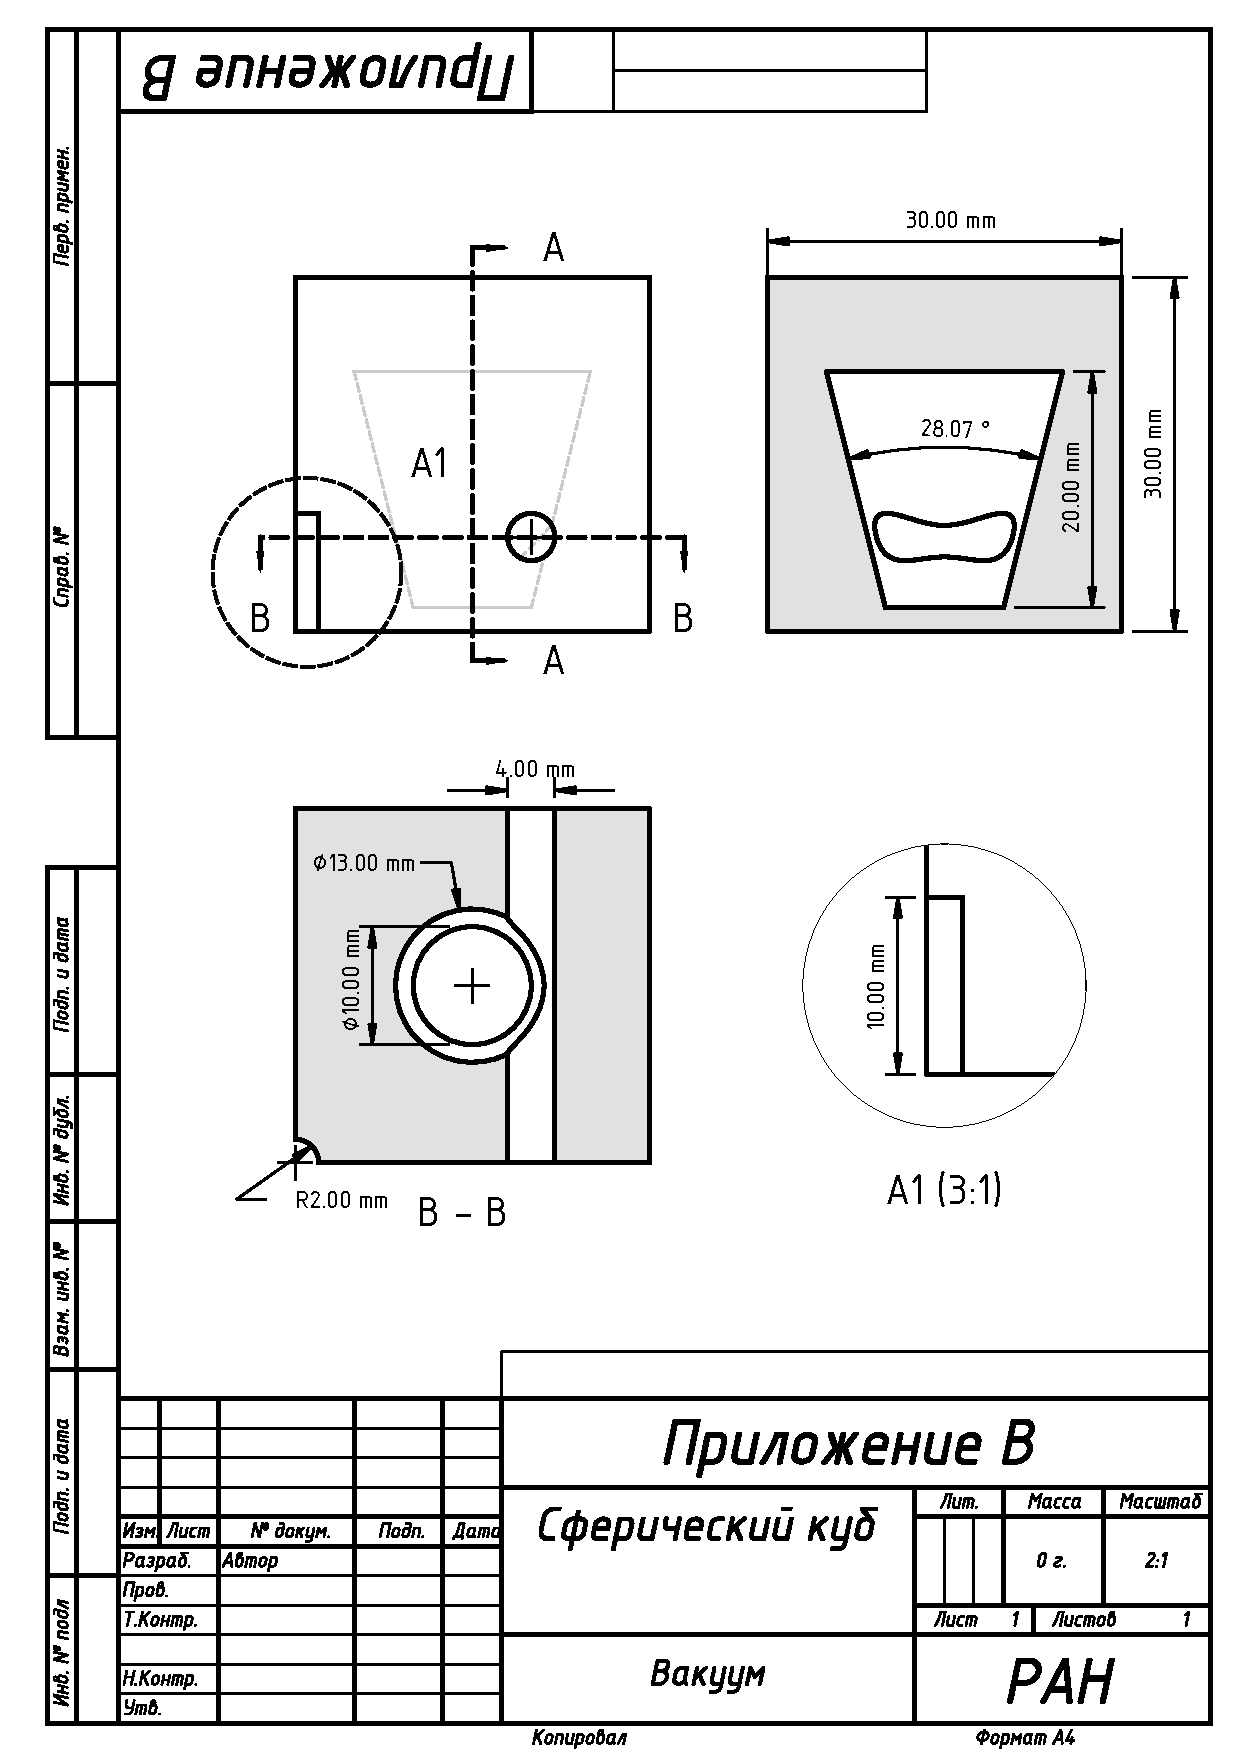
\includepdf[pages=-]{Dissertation/images/drawing.pdf}
        % Приложения

\setcounter{totalappendix}{\value{chapter}} % Подсчёт количества приложений

\end{document}
